\documentclass[a4paper,12pt]{ThesisStyle}
\usepackage[utf8]{inputenc}
\usepackage{thesis-style}
\usepackage{parskip}
\usepackage{beramono}
\usepackage[section]{placeins}
\usepackage{tabularx}
\usepackage{float}
\usepackage{xcolor}
\usepackage{colortbl}
\usepackage[labelfont=bf]{caption}
\usepackage{booktabs}
\usepackage{array}
\usepackage{graphicx, adjustbox}
\usepackage{tikz}

\usetikzlibrary{positioning}

\tikzset{main node/.style={circle,fill=blue!20,draw,minimum size=1cm,inner sep=0pt},}

\setlength{\headheight}{14.49998pt}
\addtolength{\topmargin}{-0.89998pt}

\definecolor{TblDef}{HTML}{FFFFE6}
\definecolor{Gray}{HTML}{E2E2E2}
\definecolor{Green}{HTML}{D5E8D4}
\definecolor{Blue}{HTML}{DAE8FC}
\definecolor{Orange}{HTML}{FFE6CC}
\definecolor{Purple}{HTML}{E1D5E7}

\renewcommand\tabularxcolumn[1]{m{#1}}

\begin{document}

\frontmatter

\pagenumbering{gobble}

\thispagestyle{empty}
\begin{table}[htb]
  \centering
  \begin{Large}
    \resizebox{\textwidth}{!}{\begin{tabular}{| l |}
        \hline
        \\
        
\includegraphics[scale=0.9]{/assets/logos/EPS.png}                                 \\[0.7cm]
        \centerline{Projecte de fi de grau}                                                \\[1cm]
        \hline
        \\
        \textbf{Estudi}: Grau en Enginyeria Informàtica                                    \\[0.7cm]
        \hline
        \\
        \textbf{Títol}: Eina de suport per a l’elaboració dels horaris dels graus de l’EPS \\[0.7cm]
        \hline
        \\
        \textbf{Document}: Memòria                                                         \\[0.7cm]
        \hline
        \\
        \textbf{Alumne}: Adrià Ribas Chico                                                 \\[0.7cm]
        \hline
        \\
        \textbf{Tutora 1}: Dra. Marta Fort Masdevall                                        \\
        \textbf{Departament}: Informàtica, matemàtica aplicada i estadística               \\
        \textbf{Àrea}: Llenguatges i sistemes informàtics                                  \\[0.7cm]
        \hline
        \\
        \textbf{Tutor 2}: Dr. Antonio Rodríguez Benítez                                    \\
        \textbf{Departament}: Informàtica, matemàtica aplicada i estadística               \\
        \textbf{Àrea}: Llenguatges i sistemes informàtics                                  \\[0.7cm]
        \hline
        \\
        \textbf{Convocatòria (mes/any)}: Juny de 2022                                      \\[0.7cm]
        \hline
      \end{tabular}}
  \end{Large}
\end{table}

\newpage

\begin{titlepage}

  % Upper part of the page
  
\includegraphics[scale=0.9]{/assets/logos/EPS.png} \\[1cm]
  \begin{center}
    \textsc{\Large Projecte Fi de Grau} \\[1cm]

    % Title
    \begin{spacing}{2}
      \HRule \\
      \textbf{\Huge Eina de suport per a l’elaboració dels horaris dels graus de l’EPS} \\
      \HRule \\[0.5cm]
    \end{spacing}

    % Author and supervisor and other data
    {
    \large
    \emph{Autor:} \\
    Adrià \textsc{Ribas Chico} \\[1cm]
    Juny de 2022 \\[1cm]
    Grau en Enginyeria Informàtica \\[1cm]
    \emph{Tutors:} \\
    Dra. Marta \textsc{Fort Masdevall} \\
    Dr. Antonio \textsc{Rodríguez Benítez} \\
    }

  \end{center}
\end{titlepage}

\titlepage

\dominitoc

\pagenumbering{roman}

\chapter*{Resum}
\label{cap:resum}

Resum del projecte \ldots

\chapter*{Agraïments}
\label{cap:agraiments}

Agraïments \ldots


\tableofcontents

%\listoffigures

%\listoftables

\mainmatter

\chapter{Introducció}
\label{cap:intro}

\section{Antecedents}
\label{sec:antecedents}

En aquesta secció, es resumiran els antecedents que han donat peu al plantejament d'aquest projecte.

La idea del projecte neix de determinades necessitats que cert personal de l'Escola Politècnica Superior de la Universitat de Girona fa temps que té. Més concretament, es tracta d'una necessitat del personal encarregat de gestionar tot el que fa referència a la confecció i manteniment dels horaris del centre: horaris dels graus, dels professors, ocupació d'aules i espais, etc.

Actualment, per dur a terme l'elaboració dels horaris, aquestes persones utilitzen mètodes i eines incòmodes i poc àgils, a part de no estar automatitzades ni específicament dissenyades per abordar aquest tipus de tasques. Tampoc existeix cap plataforma que unifiqui les fases d'aquest procés de gestió ni que n'estableixi una manera de fer comuna.

Ara per ara, per exemple, no tenen manera de detectar incompatibilitats horàries ni solapaments \textit{a priori} de manera automàtica. Degut a això, en moltes ocasions s'han de repetir certes fases del procés fins que el resultat és vàlid i la gent implicada hi està d'acord.

Al capítol~\ref{cap:marcdetreball} es descriurà amb més profunditat com funcionen avui dia aquests processos d'elaboració i gestió d'horaris de l'escola.

\section{Propòsit}
\label{sec:proposit}

En aquesta secció, s'exposarà el propòsit general del projecte, tenint en compte els antecedents vists a la secció~\ref{sec:antecedents}.

En definitiva, la gestió dels horaris de l'EPS suposa una inversió de temps massa elevada per a la gent que se n'ocupa. És per això que Marta Fort Masdevall, coordinadora d'estudi del Grau en Enginyeria Informàtica de la universitat, proposa un projecte de fi de grau que té la finalitat de trobar una solució al problema.

El propòsit és desenvolupar una eina de suport informàtic que permeti a l'usuari elaborar horaris de forma àgil, eficient i segura. L'eina també hauria de ser capaç de comprovar automàticament la disponibilitat de les aules, les incompatibilitats horàries dels professors i la concordança entre les assignatures i el nombre de grups previstos. A més a més, hauria d'oferir diverses vistes per tal que l'usuari pugui visualitzar la informació, com ara:
\begin{itemize}
  \item Els horaris d'un grau per curs i quadrimestre.
  \item Els horaris d'un professor per quadrimestre.
  \item L'ocupació d'un espai per quadrimestre.
\end{itemize}

També es planteja la possibilitat de disposar d'un sistema de control d'usuaris. Cada usuari tindria assignat un conjunt de rols determinat. Els rols representarien els diferents càrrecs del personal de l'EPS en matèria de gestió d'horaris. Així doncs, cada usuari podria executar les accions i consultar la informació que el seu conjunt de rols li permeti. D'aquesta manera, es dividirien les diferents tasques i processos entre rols d'usuari i cadascun dels càrrecs podria realitzar la feina que li correspon. La proposta inicial comprèn els rols d'usuari següents:
\begin{itemize}
  \item \texttt{Administrador}: Introdueix les dades dels plans docents i dóna d'alta Coordinadors i Directors de departament.
  \item \texttt{Coordinador}: Elabora els horaris.
  \item \texttt{Director de departament}: Dóna d'alta Responsables de docència.
  \item \texttt{Responsable de docència}: Dóna d'alta i assigna Professors als grups.
  \item \texttt{Professor}: Visualitza el seu horari.
\end{itemize}

A més a més, l'aplicació hauria de ser accessible via web. D'aquesta manera, tots els usuaris podrien utilitzar-la des de qualsevol lloc i dispositiu, sense preocupar-se d'instal·lacions ni actualitzacions.

\section{Motivacions}
\label{sec:motivacions}

En aquesta secció, es parlarà en primera persona sobre quines motivacions personals hi ha darrere del projecte i en justifiquen l'elecció.

Un dels aspectes que més em motiven de la informàtica en general és el fet de poder ajudar la gent a estalviar el seu temps, el qual té un gran valor. En moltes ocasions, una persona, un grup o fins i tot una institució, inverteix una quantitat elevada de temps en realitzar certes accions o activitats, sigui en l'àmbit que sigui. Aquest temps es pot reduir si l'acció o activitat en qüestió té una part suficientment mecànica. Tanmateix, encara que no la tingui, sovint és possible desenvolupar una eina informàtica que n'augmenti l'eficiència o, si més no, dinamitzar-la i fer que resulti més còmoda i pràctica.

D'aquí sorgeix el meu objectiu principal pel que fa a la informàtica, que és precisament aportar el meu gra de sorra a aquesta causa.

Per aquest motiu, m'ha cridat molt l'atenció la proposta d'aquest projecte. És una molt bona oportunitat per contribuir a millorar el procés de gestió i elaboració d'horaris de l'escola, que sol resultar bastant costós en temps per a les persones que hi participen.

D'altra banda, em motiva molt el fet de desenvolupar una aplicació que podrà ser implantada en un entorn real i que podrà beneficiar les persones que la facin servir. No em cridaria tant dur a terme un altre projecte que, un cop finalitzat, fos simplement arxivat, sense utilitat pràctica per a ningú més excepte per a mi, que seria l'únic que me'n beneficiaria, ja que igualment obtindria coneixements i experiència.

Actualment i cada vegada més, m'interessa el desenvolupament d'entorns web. És per això que un factor decisiu a l'hora d'escollir aquesta proposta de PFG ha estat que un dels requisits sigui desenvolupar-lo en format de plataforma web.

\section{Objectius generals}
\label{sec:objectius_generals}

En aquesta secció, s'enumeraran els objectius generals del projecte, que ja s'han deixat entreveure prèviament a la secció~\ref{sec:proposit}. No obstant això, a continuació se'n presenta la llista completa:
\begin{itemize}
  \item Proporcionar una interfície còmoda i intuïtiva per dur a terme les tasques de gestió i elaboració dels horaris de l'EPS.
  \item Emmagatzemar i processar dinàmicament les dades i relacions referents als diversos graus, cursos, quadrimestres, assignatures, grups, espais, professors, etc.
  \item Detectar i evitar automàticament qualsevol tipus d'inconsistència o incompatibilitat horària, per tal d'aportar seguretat al treball.
  \item Possibilitar la pujada d'arxius externs de dades que serveixin per obtenir la informació bàsica necessària per al funcionament de l'aplicació i generar possibles punts de partida per a la planificació dels horaris.
  \item Permetre la visualització de l'ocupació de les aules, dels horaris dels professors i dels horaris dels grups de cada grau, entre d'altres vistes que puguin ser d'utilitat pels usuaris.
  \item Admetre diferents rols d'usuari, als quals s'assigni una sèrie de tasques i un conjunt de permisos concret.
\end{itemize}

Al capítol~\ref{cap:requisits} es desenvoluparan aquests objectius generals i es concretaran els requisits específics de l'aplicatiu.

AFEGIR QUE S'HAN DE LLEGIR LES DADES DEL PLA DOCENT!


%%%%%%%%%%%%%%%%%%%%%%%%%%%%%%%%%%%%%%%%%%%%%%%%%%%%%%%%%%%%%%%%%%%%%%%%%%%%%%%%%%%%%%%%%%%%%%%%%%%%%%%%%%%%%%%%%%%%%%%%%%%%%%%%%%%%%%%%%%%%%%%%%%%%%
\section{-------------- EXEMPLES I UTILITATS --------------}
\subsection{Paraules per començar seccions}

Abordar, concretar, exposar, parlar, descriure, repassar, mostrar, ensenyar, desenvolupar, tractar, veure, aprofundir, investigar, discutir, indagar, detallar, enumerar,

\subsection{Altres}

Exemple de taula:
\begin{table}[htb]
  \centering
  \begin{tabular}{ | r | c | c | l | }
    \hline
    Any  & Matriculats & Aprovats & Percentatge \\
    \hline
    2019 & 65          & 47       & 72.3\%      \\
    2020 & 69          & 48       & 69.6\%      \\
    2021 & 75          & 58       & 77.3\%      \\
    \hline
  \end{tabular}
  \caption{\label{taula:taulaexemple} Aquí és on s'ha de posar el peu de taula. }
\end{table}

Exemple de figura:
\begin{figure}[htb]
  \centering
  
\includegraphics[width=8 cm]{/assets/logos/EPS.png}
  \caption{\label{fig:logo} Logotip de l'Escola Politècnica Superior.}
\end{figure}

Exemple de fòrmula:
\begin{equation}
  H(X) = -\sum_{i=1}^{N}p_s(x_i) \log \left( p_s(x_i) \right).
  \label{equ:entropia}
\end{equation}


També es pot fer referència en el text a les taules (p.ex. veure la Taula~\ref{taula:taulaexemple}), a les figures (p.ex. veure la Figura~\ref{fig:logo}) o a les fòrmules (p.ex. veure Equació~\ref{equ:entropia}).

%%%%%%%%%%%%%%%%%%%%%%%%%%%%%%%%%%%%%%%%%%%%%%%%%%%%%%%%%%%%%%%%%%%%%%%%%%%%%%%%%%%%%%%%%%%%%%%%%%%%%%%%%%%%%%%%%%%%%%%


\chapter{Estudi de viabilitat}
\label{cap:viabilitat}

\section{Costos de personal}
\label{sec:costos_personal}

En aquesta secció, es calcularan els costos relatius al personal que participa en el desenvolupament del projecte.

Com que es tracta d'una aplicació web, és necessari diferenciar entre les persones que desenvolupen la part del servidor (\textit{back-end}) i les que desenvolupen la del client (\textit{front-end}).

Tal com es veurà al capítol~\ref{cap:estudi}, la tecnologia escollida per al \textit{back-end} és Node.js, mentre que l'escollida per al \textit{front-end} és Vue.js. Per tant, els preus que es tindran en compte als càlculs són els de desenvolupadors Node.js i desenvolupadors \textit{front-end} JavaScript en general.

A més a més, tenint en compte la importància que prèn per al projecte el disseny de les interfícies d'usuari, cal comptar també amb dissenyadors d'interfícies.

\begin{table}[H]
  \begin{tabularx}{\textwidth}{X  r  c  r}
    \toprule
    \rowcolor{TblDef}
    \textbf{Personal}                               & \textbf{Temps}      & \textbf{Preu}   & \textbf{Cost total}\\
    \midrule[0.9pt]
    Desenvolupadors Node.js                         & 258 hores           & 18.00 €/hora    & 4644.00 € \\
    \midrule
    Desenvolupadors \textit{front-end} JavaScript   & 243 hores           & 15.15 €/hora    & 3681.45 € \\
    \midrule
    Dissenyadors d'interfícies                      & 87 hores            & 14.68 €/hora    & 1277.16 € \\
    \midrule[0.9pt]
    \textbf{Total}                                  & \textbf{588 hores}  &                 & \textbf{9602.61 €} \\
    \bottomrule
  \end{tabularx}
  \caption{\label{taula:costos_personal} Taula de costos de personal.}
\end{table}

El temps de dedicació estimat dels diferents tipus de personal s'ha extret del capítol~\ref{cap:planificacio}. Cal remarcar que el temps dedicat a la gestió del projecte s'ha tingut en compte per al càlcul del temps dels desenvolupadors.

L'estimació dels preus dels diferents tipus de personal s'ha obtingut de l'informe de salaris de la \emph{Guia HAYS 2022}~\cite{Hays}.

\chapter{Metodologia}
\label{cap:metodologia}



\chapter{Marc de treball i conceptes previs}
\label{cap:marcdetreball}

\section{¿¿¿Funcionament actual???}
\label{sec:funcionament_actual}

En aquesta secció, es detallaran quins són i com funcionen els mètodes de gestió i elaboració d'horaris de l'EPS que s'utilitzen actualment. Es veuran quins càrrecs de l'escola hi participen i les seves funcions, així com la manera en què interactuen entre ells i intercanvien la informació corresponent.

------------------------

Idees

Parlar del flux dels processos, etc \ldots

Rectorat reparteix crèdits a les facultats. Cada facultat decideix quants grups grans, petits, etc. de cada grau en funció dels alumnes. Introdueix els excels.
A partir d'aquí, entren els coordinadors, per fer els horaris amb els seus mètodes. Canviar-los el mínim possible respecte l'any passat, per intentar evitar
solapaments. Un cop fets, els coordinadors passen els horaris a direcció. S'entren al sistema i revisen solapaments. Si tot està bé, els responsables de docència,
que assignen professors als grups.

Grups grans i mitjans no hi ha restriccions d'aules. Grups petits sí,

------------------------

\section{Nomenclatura específica}
\label{sec:nomenclatura}

En aquesta secció, es definirà la nomenclatura específica del marc de treball del projecte: el procés de gestió dels horaris de la UdG aplicat a l'Escola Politècnica Superior. Aquesta nomenclatura es farà servir en la resta de la memòria.

\begin{itemize}
  \item \texttt{Facultat:} Secció d'una universitat a la qual correspon una branca general de coneixement, com ara ``Escola Politècnica Superior'' o ``Facultat de Medicina'' de la UdG.
  \item \texttt{Curs acadèmic:} Període de temps format per l'últim quadrimestre d'un any i el primer del següent.
  \item \texttt{Pla docent:} Instrument que defineix la informació clau sobre els estudis que es cursen en una facultat durant un curs acadèmic. Les dades més rellevants que contenen els de l'EPS són les següents:
  \begin{itemize}
    \item Per a cada assignatura:
    \begin{itemize}
      \item Estudis als quals pertany
      \item Codi
      \item Nom
      \item Àrees a les quals pertany
      \item Departament al qual pertany cadascuna de les àrees
      \item Tipus de laboratori que té assignats
      \item Crèdits
      \item Nombre de grups grans
      \item Nombre de grups mitjans
      \item Nombre de grups petits
    \end{itemize}
    \item Per a cada tipus de laboratori:
    \begin{itemize}
      \item Nom
      \item Quantitat d'aules
      \item Capacitat d'alumnes
    \end{itemize}
  \end{itemize}
  \item \texttt{Departament:} Grup destinat a la recerca i a l'ensenyament d'una matèria determinada en una o diverses facultats sota la direcció d'un director, com ara ``Informàtica, Matemàtica Aplicada i Estadística'' de l'EPS.
  \item \texttt{Àrea:} Marc d'estudi concret dins de la matèria d'un departament sota la gestió d'un responsable, com ara ``Llenguatges i Sistemes Informàtics'' del departament d'IMAE.
  \item \texttt{Estudi:} Terme que engloba els diferents tipus d'estudis universitaris (ja siguin graus, màsters, etc.) com ara el ``Grau en Enginyeria Informàtica''. Un estudi pertany a una facultat concreta i és gestionat per un coordinador.
  \item \texttt{Curs:} Any d'escolaritat d'un estudi que agrupa assignatures repartides en dos quadrimestres (anomenats respectivament primer i segon), com ara ``tercer curs'' o ``quart curs'' de GEINF.
  \item \texttt{Quadrimestre:} Espai de quatre mesos corresponent al final d'un any (primer quadrimestre) o bé a l'inici del següent (segon quadrimestre).
  \item \texttt{Assignatura:} Conjunt de coneixements d'una matèria que es cursa cada any durant un quadrimestre concret, com ara ``Estadística''. Cada assignatura pertany a una o múltiples àrees i s'imparteix a un o diversos estudis, però no necessàriament en el mateix curs. A més a més, té assignat un conjunt de tipus de laboratori concret.
  \item \texttt{Tipus de laboratori:} Grup de laboratoris que comparteixen les mateixes característiques i finalitats, com ara ``Infor''. Cada tipus de laboratori té definides tant la quantitat d'aules existent com la capacitat d'alumnes.
  \item \texttt{Aula:} Espai en el qual s'imparteix docència, com ara ``PI-01''.
  \item \texttt{Grup:} Concepte que es refereix a un grup de qualsevol tipus (gran, mitjà o petit) d'una assignatura determinada, com ara el ``grup gran 1'' d'Estadística. Una assignatura està composta per un nombre concret de grups de cada tipus i els grups d'un mateix tipus es numeren successivament per tal de distingir-los. A més, en el cas d'una assignatura compartida entre múltiples estudis, cadascun dels seus grups està assignat a un dels estudis o, fins i tot, a més d'un.
  \item \texttt{Bloc horari:} Instància d'un grup determinat assignable a un horari, com ara el ``bloc horari 2'' del grup gran 1 d'Estadística. S'entén per assignació a un horari el fet de situar-hi un bloc horari en una setmana, dia i hora d'inici concrets. Cadascun conté la informació següent:
  \begin{itemize}
    \item Grup al qual pertany
    \item Dia (en cas que estigui assignat)
    \item Hora d'inici (en cas que estigui assignat)
    \item Duració
    \item Setmana o setmanes
    \item Professor que hi imparteix docència
    \item Aula en la qual s'imparteix la docència
  \end{itemize}
  En la majoria de casos, un grup disposa d'un sol bloc horari, encara que és possible que un grup faci més d'una classe a la setmana i, per tant, hagi de disposar de més d'un bloc horari. 
  \item \texttt{Bloc horari genèric:} Bloc horari que no pertany a un grup, sinó directament a un quadrimestre d'un dels cursos d'un estudi, com ara la ``Franja Reservada per a Proves d'Avaluació Continuada'' del primer quadrimestre de tercer de GEINF. Cadascun conté la informació següent:
  \begin{itemize}
    \item Estudi al qual pertany
    \item Curs
    \item Quadrimestre
    \item Etiqueta. Per exemple: ``Franja Reservada per a Proves d'Avaluació Continuada''
    \item Subetiqueta. Per exemple: ``PAC''
    \item Dia (en cas que estigui assignat)
    \item Hora d'inici (en cas que estigui assignat)
    \item Duració
    \item Setmana o setmanes
  \end{itemize}
  \item \texttt{Setmana}: Concepte que fa referència als tipus amb els quals la universitat cataloga les setmanes (A o B). Un quadrimestre està format per setmanes A i per setmanes B. Per aquest motiu, els horaris dels dos tipus de setmana no han de ser necessàriament iguals i un bloc horari pot estar assignat a una setmana concreta o a les dues alhora.
  \item \texttt{Vista setmanal:} Vista de l'horari d'una setmana concreta o de la combinació de les dues. Les tres vistes possibles són les següents:
  \begin{itemize}
    \item General (conformada per blocs horaris assignats o a una de les setmanes o bé a totes).
    \item Setmanes A (conformada per blocs horaris assignats a setmanes A).
    \item Setmanes B (conformada per blocs horaris assignats a setmanes B).
  \end{itemize}
  \item \texttt{Solapament de blocs horaris:} Coincideixen múltiples blocs horaris pertanyents al mateix grup.
  \item \texttt{Solapament de tipus de laboratori:} Excés d'aules d'un tipus de laboratori concret ocupades alhora.
  \item \texttt{Solapament de professors:} Coincideixen múltiples blocs horaris amb el mateix professor assignat.
  \item \texttt{Solapament d'aules:} Coincideixen múltiples blocs horaris amb la mateixa aula assignada.
  \item \texttt{Administrador:} Persona encarregada de gestionar un pla docent i de controlar Coordinadors i Directors de departament.
  \item \texttt{Coordinador:} Persona encarregada de gestionar un estudi i d'elaborar-ne els horaris.
  \item \texttt{Director de departament:} Persona encarregada de dirigir un departament i de controlar els Responsables de docència de les seves àrees.
  \item \texttt{Responsable de docència:} Persona encarregada de gestionar una àrea i de controlar-ne els Professors.
  \item \texttt{Professor:} Persona encarregada d'impartir docència.
\end{itemize}

\section{Document d'un pla docent}
\label{sec:document_pla_docent}

En aquesta secció, es descriurà com és el format dels documents que conten un pla docent i que, tal com s'ha introduit al capítol~\ref{cap:intro}, l'aplicació ha de poder processar correctament.

Es tracta de fitxers en format \emph{xlsx} (Microsoft Excel) que contenen diversos fulls: un per les assignatures de cada estudi, un per cada agrupació d'assignatures compartides i un pels tipus de laboratori. El nom del full d'un estudi és la seva pròpia abreviació i el de tipus de laboratori és ``Laboratoris''. Pel que fa al d'una agrupació d'assignatures compartides, no existeix una convenció determinada. Actualment n'hi ha quatre:
\begin{itemize}
  \item \texttt{Comp\_ARQ}: Recull les assignatures compartides entre els estudis GARQ i GATE.
  \item \texttt{Compartides}: Recull les assignatures compartides entre els estudis GETI, GEB, GEM, GEE, GEEIA, GEQ.
  \item \texttt{ComAlim}: Recull les assignatures compartides entre els estudis GEA i GINSA.
  \item \texttt{ComInf}: Recull les assignatures compartides entre els estudis GEINF i GDDV.
\end{itemize}

Cadascun dels fulls que contenen assignatures s'organitzen en forma de taula de manera que les files corresponen a assignatures i les columnes als seus atributs. Els atributs rellevants per a l'aplicació són els següents:
\begin{itemize}
  \item \texttt{Codi:} Codi identificador.
  \item \texttt{Assignatura:} Nom.
  \item \texttt{Àrea:} Àrea a la qual pertany.
  \item \texttt{Dept:} Departament al qual pertany l'àrea.
  \item \texttt{Curs:} Curs durant el qual s'imparteix.
  \item \texttt{Sem:} Semestre durant el qual s'imparteix.
  \item \texttt{Cr.:} Nombre de crèdits.
  \item \texttt{NGG:} Nombre de grups grans.
  \item \texttt{NGM:} Nombre de grups mitjans.
  \item \texttt{NGP:} Nombre de grups petits.
  \item \texttt{Labs:} Nom del tipus de laboratori al qual s'imparteix.
\end{itemize}

Existeixen casos en què una assignatura pertany a més d'una àrea i/o s'imparteix a més d'un tipus de laboratori. En aquestes situacions, l'assignatura ocupa més d'una fila amb l'objectiu d'especificar les diferents àrees i tipus de laboratori.

A més a més, és important destacar que una assignatura compartida pot cursar-se a cursos diferents en funció de l'estudi. En aquests casos, els cursos s'indiquen separats per ``/''. L'ordre d'estudis amb el qual s'especifiquen depèn de quina agrupació d'assignatures compartides es tracti:
\begin{itemize}
  \item \texttt{Comp\_ARQ}: <curs de GARQ>/<curs de GATE>
  \item \texttt{Compartides}: Totes les assignatures es cursen durant el mateix curs.
  \item \texttt{ComAlim}: <curs de GEA>/<curs de GINSA>
  \item \texttt{ComInf}: <curs de GEINF>/<curs de GDDV>
\end{itemize}

A la figura~\ref{img:frag_pla_docent} es pot veure un fragment del full que conté les assignatures de GEINF.

\begin{figure}[H]
  \centering
  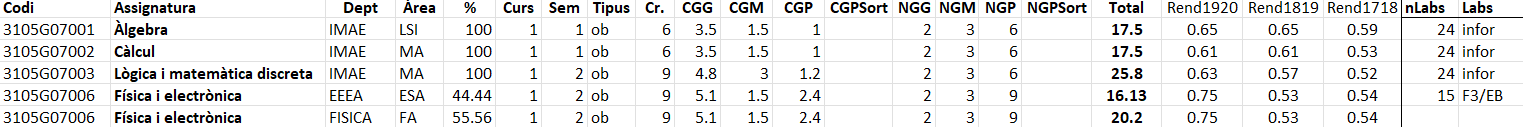
\includegraphics[width=\textwidth]{assets/figs/fitxerPlaDocent.png}
  \caption{\label{img:frag_pla_docent}Fragment del full d'un estudi d'un fitxer de pla docent.}
\end{figure}

% Citar introducció

\section{Conceptes tècnics}
\label{sec:conceptes_tecnics}

\subsection{Introducció}
\label{subsec:intro_conceptes_tecnics}

En aquesta subsecció, s'introduiran els temes i els conceptes que es tractaran a la resta de la secció.

Tal com s'ha esmentat al capítol~\ref{cap:intro}, la solució informàtica al problema que planteja el projecte s'ha d'implementar en format de plataforma o aplicació web. Si aquest requisit es suma al fet que l'emmagatzematge de dades és totalment necessari, ràpidament es pot concloure que l'arquitectura del sistema és de naturalesa client-servidor i que, consegüentment, es divideix en dues parts diferenciades (veure figura~\ref{img:esquema_web}): l'aplicació client o \textit{front-end} i l'aplicació servidor o \textit{back-end}.

\begin{figure}[H]
  \centering
  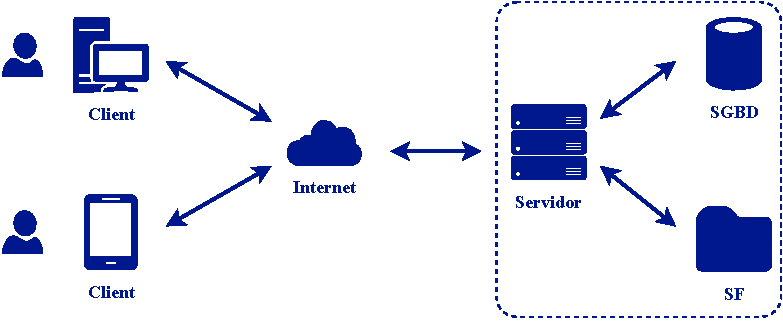
\includegraphics[width=0.95\textwidth]{assets/figs/esquemaWeb.pdf}
  \caption{\label{img:esquema_web}Esquema de l'arquitectura d'una aplicació web convencional.}
\end{figure}

L'aplicació client s'executa sobre un navegador web i s'encarrega principalment d'interactuar amb l'usuari, de manera que pugui visualitzar i manipular les dades emmagatzemades al servidor. Per poder accedir a aquestes dades, l'aplicació client ha de ser capaç de comunicar-se a través d'Internet amb l'aplicació servidor, ja que s'executa a la màquina de l'usuari.

L'aplicació servidor s'executa fora del navegador en una màquina remota. S'encarrega principalment d'atendre i servir les peticions de consulta o manipulació de dades que rep de les aplicacions client. Davant de cada petició, l'aplicació executa la lògica de negoci corresponent i persisteix les dades necessàries al SF (sistema de fitxers) o a la base de dades, la qual és operada per un SGBD (sistema gestor de bases de dades). A més a més, a part de simplificar el desenvolupament de l'aplicació client, impedeix l'accés directe a la base de dades des d'Internet, fet que seria molt perillós.

\subsection{Aplicació client}

En aquesta subsecció, es donaran a conèixer les tecnologies involucrades en el desenvolupament d'aplicacions web client.

Les aplicacions web s'executen sobre un navegador i, generalment, estan compostes pels tres elements bàsics següents:
\begin{itemize}
  \item HTML (\textit{HyperText Markup Language})~\cite{HTML}: Llenguatge de marcat que defineix la semàntica i l'estructura del contingut d'una pàgina web.
  \item CSS (\textit{Cascade Style Sheets})~\cite{CSS}: Llenguatge de fulls d'estil que defineix els estils i la presentació d'un document HTML.
  \item JS (\textit{JavaScript})~\cite{JS}: Llenguatge de programació que defineix la lògica i el comportament del contingut d'una pàgina web i la fa interactiva. Es tracta d'un llenguatge d'un sol fil d'execució, que té suport per a programació orientada a objectes, imperativa i declarativa i que pot ser interpretat o compilat en temps d'execució.
\end{itemize}

Per poder desenvolupar una aplicació web interactiva i dinàmica, en la gran majoria dels casos és necessari treballar amb el DOM mitjançant JavaScript.

El DOM (\textit{Document Object Model}) és una interfície per a documents HTML que n'estructura els elements en forma d'arbre i permet crear-hi, modificar-hi o esborrar-hi nodes, els quals representen un element HTML determinat. A través d'aquesta interfície és possible mutar en temps real el document HTML que el navegador està presentant.

Treballar directament i de manera adequada amb el DOM requereix una comprensió molt profunda del seu funcionament. A mesura que augmenta el dinamisme de l'aplicació i s'implementen interaccions més complexes, el seu desenvolupament es complica notablement i la seva mantenibilitat disminueix. A més a més, requereix una quantitat de temps considerable.

Degut a aquests motius, eventualment van sorgir els \textit{frameworks} JavaScript amb l'objectiu de brindar una millor experiència de desenvolupament i augmentar la mantenibilitat i l'escalabilitat de les aplicacions web.

Un \textit{framework} JavaScript és una infraestructura de \textit{software} que proporciona un conjunt d'eines implementades i provades que serveixen de base per crear aplicacions interactives i escalables. Els \textit{frameworks} abstreuen la gestió del DOM per tal d'estalviar al desenvolupador el fet d'haver de manipular-lo directament en la majoria d'ocasions.

Actualment, existeixen un munt de \textit{frameworks} per escollir. La majoria funcionen de manera similar, però realitzen algunes tasques de manera diferent. Cadascun té els seus avantatges i inconvenients i pot estar enfocat a un tipus d'aplicació concret, cosa que provoca que no n'existeixi un de definitiu. A la pràctica, l'opció més viable sempre depèn del tipus d'aplicació que s'hagi d'implementar. Avui dia, els més populars són React JS, Vue JS, Angular JS i Ember JS, entre d'altres.

Quan es treballa amb aquest tipus de \textit{software} i altres biblioteques de codi, de seguida apareix la necessitat d'unes eines anomenades \textit{bundlers} o ``empaquetadors''.

Abans que els mòduls ES (que permeten la importació i exportació de fragments de codi JavaScript) estéssin disponibles per a navegadors web, els desenvolupadors no tenien cap mecanisme natiu per crear codi JavaScript de manera modular. Per aquest motiu, l'ús de \textit{bundlers} sempre havia sigut necessari per tal de concatenar el codi de \textit{frameworks} i biblioteques en arxius que poguéssin ser executats en el navegador. WebPack, Rollup i Parcel són uns dels \textit{bundlers} més populars.

\subsection{Aplicació servidor}

En aquesta subsecció, es donaran a conèixer les tecnologies involucrades en el desenvolupament d'aplicacions servidor.

A diferència de les aplicacions web client, les aplicacions servidor no estan tan limitades pel que fa a llenguatges de programació. Pràcticament es poden desenvolupar fent servir qualsevol llenguatge. No obstant això, tampoc es lliuren de la necessitat de l'existència de \textit{frameworks} que proporcionin eines que rellevin el desenvolupador en les tasques més comunes, complicades o de baix nivell.

Actualment, hi ha una gran varietat d'opcions a l'hora d'escollir la tecnologia amb la qual s'ha de desenvolupar una determinada aplicació servidor. La tria depèn de múltiples factors, com ara quina és la càrrega de peticions esperada o quina importància té el rendiment envers altres aspectes. Avui dia, els més populars són Firebase, Express.js, Spring Boot, Laravel, Django i Ruby on Rails, entre d'altres.

\subsection{Comunicació entre client i servidor}

En aquesta subsecció, es parlarà sobre com s'estableix la comunicació entre l'aplicació client i l'aplicació servidor.

Tal com s'ha pogut veure anteriorment en la secció, l'existència d'eines que permetin implementar la comunicació entre diferents aplicacions és completament essencial. Aquestes eines reben el nom d'API (\textit{application programming interface}) i consisteixen un conjunt de normes i protocols que permeten la comunicació entre dues aplicacions, la qual es realitza mitjançant peticions i respostes.

En el cas de la comunicació entre el \textit{front-end} i el \textit{back-end} d'una aplicació web, es necessiten API enfocades a l'obtenció i manipulació de dades. Al llarg del temps, han sorgit diversos protocols i arquitectures que permeten desenvolupar aquesta tipologia d'API, com ara XML-RPC, SOAP, JSON-RPC, REST o GraphQL.

Actualment, l'opció més popular i utilitzada pel desenvolupament d'aquest tipus d'API és REST (\textit{Representational State Transfer})~\cite{REST}. A diferència d'altres opcions com SOAP, REST no és ni un protocol ni un estàndard, sinó un conjunt de pautes pel que fa a l'arquitectura. Una API és considerada una ``RESTful API'' o ``API REST'' si satisfà tots els principis REST~\cite{REST_CONSTRAINTS}.

Tal com el seu nom indica, quan el client llança una petició contra una API REST, l'API li transfereix una representació de l'estat actual del recurs demanat. La informació s'entrega mitjançant el protocol HTTP (\textit{Hypertext Transfer Protocol})~\cite{HTTP} i en format JSON, XML o HTML, entre d'altres. El format més usat és JSON (\textit{JavaScript Object Notation})~\cite{JSON}, ja que és fàcilment comprensible tant per màquines com persones i, a més, no depèn de cap llenguatge de programació, encara que el seu nom pugui indicar el contrari.

\subsection{Emmagatzematge i gestió de dades}

En aquesta subsecció, es parlarà sobre com es gestiona l'emmagatzematge de les dades a la banda del servidor.

En els últims anys, les dades s'han convertit en un dels punts més crítics de qualsevol aplicació. La importància d'una bona administració de les dades és clau i beneficiosa tant per a l'usuari del \textit{software} com per a l'organització que l'ha desenvolupat.

No obstant això, aconseguir portar-ho a la pràctica no és tasca senzilla. Aquí és on entren en joc els SGBD (sistemes gestors de bases de dades). Un SGBD és un tipus de programari dedicat a fer d'interfície entre la base de dades i els seus usuaris. Permet administrar, emmagatzemar i recuperar la informació d'una base de dades de manera pràctica, eficient i segura. A més a més, poden implementar funcionalitats addicionals molt útils, com ara visualització de les dades o replicació.

Generalment s'accedeix a les dades mitjançant llenguatges de consulta, com ara SQL (\textit{Structured Query Language}).

Una de les característiques més rellevants dels SGBD és que han de complir sí o sí tots els principis ACID (\textit{Atomicity, Consistency, Isolation, Durability}). Això garantitza la fiabilitat de les seves transaccions, enteses com operacions compostes per d'altres que són individuals. Més concretament, els principis ACID són els següents:
\begin{itemize}
  \item \texttt{Atomicitat:} D'una transacció o se n'executen totes les operacions que la conformen o bé no se n'executa cap.
  \item \texttt{Consistència:} L'estat en el qual es troba la base de dades quan finalitza una transacció ha de ser coherent amb l'estat que tenia abans de que comencés.
  \item \texttt{Aïllament:} Cada transacció s'ha d'executar de manera aïllada envers la resta d'operacions.
  \item \texttt{Definitivitat:} Si es confirma una transacció, el resultat ha de ser definitiu i no es pot perdre.
\end{itemize}

De nou, l'el·lecció d'un SGBD depèn en gran mesura de l'aplicació que s'hagi de desenvolupar. Existeixen un munt d'alternatives enfocades a diferents propòsits: tractament de dades relacionades, gestió de grans volums de dades, consulta molt ràpida, cerques eficients, etc.

Actualment, els SGBD més populars són Oracle, MySQL, PostgreSQL, Redis, Elasticsearch i MongoDB, entre d'altres.


\chapter{Requisits del sistema}
\label{cap:requisits}

\section{Consideracions inicials}
\label{sec:consideracions_inicials}

En aquesta secció, es presentaran una sèrie de consideracions inicials amb l'objectiu de clarificar el contingut de les seccions que segueixen.

En primer lloc, és necessari definir el format que adoptarà cadascun dels requisits del sistema:
\\[8pt]
\centerline{\texttt{\textbf{Tipus-Numeració [Prioritat]}}: Descripció}

Més concretament, el tipus de requisit es representarà mitjançant les seves sigles, com ara \texttt{RF} pels funcionals o \texttt{RNF} pels no funcionals. La numeració es dividirà en grups en funció del rol d'usuari al qual pertanyi el requisit i inclourà la inicial del nom del rol. Pel que fa a la prioritat, se n'han definit tres nivells:
\begin{itemize}
  \item Prioritat \texttt{\textbf{[1]}} o essencial: El requisit s'ha de satisfer per tal que l'aplicació funcioni correctament, a nivell elemental.
  \item Prioritat \texttt{\textbf{[2]}} o recomanable: El requisit s'hauria de satisfer per tal que l'aplicació garanteixi una bona experiència d'usuari.
  \item Prioritat \texttt{\textbf{[3]}} o opcional: El requisit es podria satisfer per tal que l'aplicació ofereixi una excel·lent experiència d'usuari.
\end{itemize}

D'altra banda, cal remarcar que les descripcions dels requisits utilitzen la nomenclatura específica del marc de treball, detallada al capítol~\ref{cap:marcdetreball}.

A més a més, per evitar explicacions redundants, d'ara en endavant, quan es parli de la visualització dels horaris d'un grau, no s'estarà fent referència a una vista del conglomerat d'horaris de tots els seus cursos i quadrimestres, sinó de vistes en què es mostra l'horari d'un quadrimestre específic en un curs específic. De la mateixa manera, la visualització dels horaris d'un professor o la de l'ocupació d'una aula es separa en quadrimestres.

\section{Requisits funcionals}
\label{sec:requisits_funcionals}

\subsection{Requisits generals}
\label{subsec:requisits_generals}

En aquesta subsecció, es llistaran els requisits funcionals generals del sistema, comuns per a tots els usuaris, independentment dels seus rols.

\begin{itemize}
  \item \texttt{\textbf{RF-G1 [1]}}: Assegurar l'autenticació de tots els usuaris a través d'un formulari de \textit{login}, que s'ha de mostrar a la pantalla quan un usuari no autenticat accedeix a l'aplicació. Sense estar-ho, no l'ha de poder fer servir. L'autenticació d'un usuari ha de suposar la generació d'un \textit{JSON Web Token}~\cite{JWT}, per tal de mantenir la seva sessió i poder ser identificat de forma segura pel procés d'autorització de l'aplicació de l'API (o servidor).
  \item \texttt{\textbf{RF-G2 [1]}}: No permetre l'autoregistre d'usuaris, ja que usuaris de determinats rols s'encarregaran de donar d'alta altres usuaris del rol que els correspongui. El procés d'alta d'usuaris es detalla a continuació:
        \begin{enumerate}
          \item L'usuari que registra introdueix les dades de l'usuari que vol donar d'alta, entre les quals consta la seva adreça de correu electrònic. A continuació, l'usuari es crea però amb l'estat de ``desactivat''.
          \item El nou usuari rep un \textit{email} de confirmació amb un enllaç. Mentrestant, no pot autenticar-se a l'aplicació, ja que encara està desactivat.
          \item Un cop l'usuari accedeix a l'enllaç, envia el \textit{token} que conté al servidor. Si és vàlid i no ha expirat, pot procedir a crear la seva contrasenya mitjançant el formulari presentat a la pantalla. La contrasenya s'emmagatzema encriptada.
        \end{enumerate}
  \item \texttt{\textbf{RF-G3 [1]}}: Posar a disposició de l'usuari l'opció de restablir, en cas de pèrdua, la seva contrasenya des de la pàgina de \textit{login}. El procediment ha d'utilitzar el seu correu electrònic com a punt de recuperació.
  \item \texttt{\textbf{RF-G4 [1]}}: Permetre als usuaris canviar la seva contrasenya àgilment, sempre i quan estiguin autenticats. Per poder-ho fer, com a mesura de seguretat també han d'indicar la contrasenya actual.
  \item \texttt{\textbf{RF-G5 [1]}}: L'aplicació del servidor ha d'integrar un mecanisme d'autorització per tal de restringir l'accés als \textit{endpoints} de l'API. Només han de poder utilitzar-los els usuaris que s'hagin autenticat prèviament i que, a més, tinguin permís per fer-ho, de manera que cada \textit{endpoint} sigui accessible només per a un conjunt d'usuaris concret.
  \item \texttt{\textbf{RF-G6 [2]}}: Possibilitar a tots els usuaris la consulta de les seves dades personals i del seu context.
  \item \texttt{\textbf{RF-G7 [1]}}: Mostrar un menú que permeti a l'usuari navegar entre les diferents pàgines que exposen les funcionalitats principals corresponents al seu rol.
  \item \texttt{\textbf{RF-G8 [1]}}: Totes les pàgines de l'aplicació han de permetre la selecció del curs acadèmic al qual l'usuari es vol situar. S'han de poder seleccionar qualsevol dels cursos acadèmics passats (que tinguin pla docent), l'actual o el següent. No obstant això, només ha de ser modificable la informació de l'actual i del següent, a excepció de l'anterior, que ha de seguir essent modificable fins el proper 30 de juny. Per exemple, la informació relacionada amb el curs acadèmic 2021 - 2022 ha de ser modificable fins el 30 de juny de 2022.
  \item \texttt{\textbf{RF-G9 [1]}}: Els registres de la base de dades no s'han d'esborrar definitivament. En comptes d'això, tots han de tenir un camp que guardi la data en què han estat eliminats, si és que s'han eliminat. Si no ho estan, aquest camp ha de ser nul.
  \item \texttt{\textbf{RF-G10 [1]}}: Per no desaprofitar espai de la memòria, una vegada la informació d'un curs acadèmic ja no es pugui modificar, s'esborraran definitivament tots els registres que tinguin data d'eliminació no nul·la de la base de dades en els quals està continguda.
\end{itemize}


% ADMINISTRADORS
\subsection{Requisits dels Administradors}
\label{subsec:requisits_administradors}

En aquesta subsecció, es llistaran els requisits funcionals particulars dels usuaris amb rol d'Administrador. Cadascun dels apartats que segueixen correspon a una de les seves funcionalitats principals.

\subsubsection{Gestió de plans docents}
\begin{itemize}
  \item \texttt{\textbf{RF-A1 [1]}}: Seleccionar un curs acadèmic i veure la informació bàsica del seu pla docent, sempre i quan ja s'hagi carregat. S'han de poder seleccionar qualsevol dels cursos acadèmics passats (que tinguin pla docent), l'actual o el següent. El període en què un curs acadèmic s'ha de considerar ``actual'' comprèn des de l'1 de juny del primer any fins el 30 d'abril del segon any. Malgrat això, podrà realitzar modificacions als No ha de poder efectuar cap acció que alteri o modifiqui dades de cursos acadèmics anteriors a l'actual. Marcar un curs acadèmic com a ``actual'', sempre i quan ja tingui un pla docent carregat.
  \item \texttt{\textbf{RF-A2 [1]}}: Si encara no ho ha fet, carregar el pla docent a partir d'un fitxer de dades.
  \item \texttt{\textbf{RF-A3 [1]}}: Tornar a pujar el pla docent. A mode de confirmació, ha d'entrar la seva contrasenya abans no s'executi el procediment.
  \item \texttt{\textbf{RF-A4 [2]}}: Esborrar el pla docent. A mode de confirmació, ha d'entrar la seva contrasenya abans no s'executi el procediment.
  \item \texttt{\textbf{RF-A5 [1]}}: Modificar un cert conjunt de paràmetres del pla docent sense haver de tornar-lo a carregar:
        \begin{itemize}
          \item Nombre d'aules habilitades de cada tipus.
          \item Nombre de grups de qualsevol assignatura.
        \end{itemize}
\end{itemize}

\subsubsection{Assignació d'aules}
\begin{itemize}
  \item \texttt{\textbf{RF-A6 [2]}}: Assignar una aula concreta a cada bloc horari que pugui realitzar-se a més d'una, a mesura que els Coordinadors acabin d'elaborar els horaris que els pertoquin.
\end{itemize}

\subsubsection{Gestió de Coordinadors}
\begin{itemize}
  \item \texttt{\textbf{RF-A7 [1]}}: Visualitzar la llista de les assignacions de Coordinador als diferents graus del curs acadèmic.
  \item \texttt{\textbf{RF-A8 [1]}}: Assignar un dels Coordinadors encara no assignats a qualsevol dels graus. Per fer efectiva l'assignació, ha de confirmar-la.
  \item \texttt{\textbf{RF-A9 [2]}}: Per defecte i automàticament, s'ha de fer una proposta inicial d'assignacions. Per a cada grau, s'ha de proposar l'assignació del mateix Coordinador que tenia al curs acadèmic anterior, amb l'objectiu d'agilitzar el procés. No obstant això, aquestes assignacions no seran efectives fins que, manualment, les hagi confirmat.
  \item \texttt{\textbf{RF-A10 [1]}}: Eliminar qualsevol de les assignacions ja confirmades.
  \item \texttt{\textbf{RF-A11 [1]}}: Visualitzar el llistat de tots els usuaris Coordinadors, juntament amb la seva informació: nom complet, adreça de correu electrònic, grau al qual està assignat aquest curs acadèmic i si està o no activat.
  \item \texttt{\textbf{RF-A12 [1]}}: Donar d'alta usuaris Coordinadors, és a dir, usuaris amb rol de Coordinador. Per fer-ho, ha d'entrar el seu nom, cognoms i adreça de correu electrònic. A continuació, es duu a terme el procés genèric explicat a la subsecció~\ref{subsec:requisits_generals}. A més a més, ha de poder reenviar-li el correu d'activació.
  \item \texttt{\textbf{RF-A13 [1]}}: Donar de baixa usuaris Coordinadors. No s'ha d'eliminar la feina que hagin fet als cursos acadèmics anteriors.
\end{itemize}

\subsubsection{Gestió de Directors de departament}
\begin{itemize}
  \item \texttt{\textbf{RF-A14 [1]}}: Visualitzar la llista de les assignacions de Director de departament als diferents departaments del curs acadèmic.
  \item \texttt{\textbf{RF-A15 [1]}}: Assignar un dels Directors encara no assignats a qualsevol dels departaments. Per fer efectiva l'assignació, ha de confirmar-la.
  \item \texttt{\textbf{RF-A16 [2]}}: Per defecte i automàticament, s'ha de fer una proposta inicial d'assignacions. Per a cada departament, s'ha de proposar l'assignació del mateix Director que tenia al curs acadèmic anterior, amb l'objectiu d'agilitzar el procés. No obstant això, aquestes assignacions no seran efectives fins que, manualment, les hagi confirmat.
  \item \texttt{\textbf{RF-A17 [1]}}: Eliminar qualsevol de les assignacions ja confirmades. Aquesta acció no ha d'afectar els usuaris que el Director en qüestió hagi donat d'alta.
  \item \texttt{\textbf{RF-A18 [1]}}: Visualitzar el llistat de tots els usuaris Directors de departament, juntament amb la seva informació: nom complet, adreça de correu electrònic, departament al qual està assignat aquest curs acadèmic i si està o no activat.
  \item \texttt{\textbf{RF-A19 [1]}}: Donar d'alta usuaris Directors de departament, és a dir, usuaris amb rol de Director de departament. Per fer-ho, ha d'entrar el seu nom, cognoms i adreça de correu electrònic. A continuació, es duu a terme el procés genèric explicat a la subsecció~\ref{subsec:requisits_generals}. A més a més, ha de poder reenviar-li el correu d'activació.
  \item \texttt{\textbf{RF-A20 [1]}}: Donar de baixa usuaris Directors de departament.
\end{itemize}

% COORDINADORS
\subsection{Requisits dels Coordinadors}
\label{subsec:requisits_coordinadors}

En aquesta subsecció, es llistaran els requisits funcionals particulars dels usuaris amb rol de Coordinador. Cadascun dels apartats que segueixen correspon a una de les seves funcionalitats principals.

\subsubsection{Gestió d'horaris de graus}
\begin{itemize}
  \item \texttt{\textbf{RF-C1 [1]}}: Visualitzar els horaris del grau que gestiona, separats en cursos i quadrimestres.
  \item \texttt{\textbf{RF-C2 [1]}}: Visualitzar els horaris dels graus que ofereixin alguna assignatura compartida amb el grau que gestiona.
  \item \texttt{\textbf{RF-C3 [1]}}: Carregar opcionalment uns horaris elaborats prèviament per tal d'omplir els actuals i tenir un punt de partida. Si els torna a carregar es substituiran.
  \item \texttt{\textbf{RF-C4 [1]}}: Editar els horaris dels quadrimestres de qualsevol dels cursos del grau que gestiona. El ventall de possibilitats del procés d'edició es detalla a continuació:
        \begin{itemize}
          \item Un cop situat un bloc horari, consultar el nombre d'aules disponibles del seu tipus restants en la franja horària en qüestió.
          \item Seleccionar una vista setmanal per tal de visualitzar els blocs horaris situats a un tipus de setmana concret. Les vistes setmanals són les següents:
                \begin{itemize}
                  \item Vista dels blocs horaris situats a les setmanes de tipus A.
                  \item Vista dels blocs horaris situats a les setmanes de tipus B.
                  \item Vista de tots els blocs horaris, independentment del tipus de setmana en què estigui situat.
                \end{itemize}
          \item Visualitzar els blocs horaris pendents de situar.
          \item Situar o moure blocs horaris a franges horàries concretes del tipus de setmana que s'estigui visualitzant.
          \item Treure blocs horaris ja situats en una franja horària, que quedaran com a pendents de situar.
          \item Crear manualment blocs horaris genèrics que no estiguin associats a cap grup de cap assignatura. Cal que n'especifiqui la seva duració, descripció i tipus.
        \end{itemize}
  \item \texttt{\textbf{RF-C5 [2]}}: Realitzar, en cas que sigui necessari, les següents modificacions sobre els paràmetres que involucren el grau que gestiona donats (inicialment) pel pla docent, amb possibilitat de desfer-les:
        \begin{itemize}
          \item Modificar la duració de qualsevol bloc horari.
          \item Modificar el número identificador de qualsevol dels grups de les assignatures.
          \item Modificar el nombre de blocs horaris de cada tipus de grup de qualsevol assignatura.
        \end{itemize}
  \item \texttt{\textbf{RF-C6 [3]}}: Descarregar la versió actual de qualsevol dels horaris que estigui elaborant.
  \item \texttt{\textbf{RF-C7 [1]}}: Conèixer en temps real les discrepàncies entre l'horari que estigui elaborant i el pla docent vigent, així com qualsevol incompatibilitat horària que pugui sorgir.
\end{itemize}

\subsubsection{Consulta d'horaris de Professors}
\begin{itemize}
  \item \texttt{\textbf{RF-C8 [1]}}: Visualitzar els horaris dels Professors que imparteixin docència a alguna de les assignatures que ofereixi el grau que gestiona.
\end{itemize}

\subsubsection{Consulta d'horaris d'aules}
\begin{itemize}
  \item \texttt{\textbf{RF-C9 [2]}}: Visualitzar els horaris de l'ocupació de qualsevol aula de l'escola.
\end{itemize}


% DIRECTORS DE DEPARTAMENT
\subsection{Requisits dels Directors de departament}
\label{subsec:requisits_director_departament}

En aquesta subsecció, es llistaran els requisits funcionals particulars dels usuaris amb rol de Director de departament. Cadascun dels apartats que segueixen correspon a una de les seves funcionalitats principals.

\subsubsection{Consulta d'horaris de Professors}
\begin{itemize}
  \item \texttt{\textbf{RF-D1 [1]}}: Visualitzar els horaris dels Professors que imparteixin docència a alguna assignatura de qualsevol de les àrees del seu departament.
\end{itemize}

\subsubsection{Consulta d'horaris de graus}
\begin{itemize}
  \item \texttt{\textbf{RF-D2 [1]}}: Visualitzar els horaris dels graus que ofereixin alguna assignatura de qualsevol de les àrees del seu departament.
\end{itemize}

\subsubsection{Gestió de Responsables de docència}
\begin{itemize}
  \item \texttt{\textbf{RF-D3 [1]}}: Visualitzar la llista de les assignacions de Responsable de docència a les diferents àrees del seu departament en un curs acadèmic.
  \item \texttt{\textbf{RF-D4 [1]}}: Assignar un conjunt de Responsables encara no assignats a qualsevol de les àrees del seu departament. Per fer efectiva l'assignació, ha de confirmar-la.
  \item \texttt{\textbf{RF-D5 [2]}}: Per defecte i automàticament, s'ha de fer una proposta inicial d'assignacions. Per a cada àrea, s'ha de proposar l'assignació del mateix Responsable que tenia al curs acadèmic anterior, amb l'objectiu d'agilitzar el procés. No obstant això, aquestes assignacions no seran efectives fins que, manualment, les hagi confirmat.
  \item \texttt{\textbf{RF-D6 [1]}}: Eliminar qualsevol de les assignacions ja confirmades. Aquesta acció no ha d'afectar els usuaris que el Responsable en qüestió hagi donat d'alta.
  \item \texttt{\textbf{RF-D7 [1]}}: Visualitzar el llistat de tots els usuaris Responsables de docència, juntament amb la seva informació: nom complet, adreça de correu electrònic, àrea a la qual està assignat aquest curs acadèmic i si està o no activat.
  \item \texttt{\textbf{RF-D8 [1]}}: Donar d'alta usuaris Responsables de docència, és a dir, usuaris amb rol de Responsable de docència. Per fer-ho, ha d'entrar el seu nom, cognoms i adreça de correu electrònic. A continuació, es duu a terme el procés genèric explicat a la subsecció~\ref{subsec:requisits_generals}. A més a més, ha de poder reenviar-li el correu d'activació.
  \item \texttt{\textbf{RF-D9 [1]}}: Donar de baixa usuaris Responsables de docència.
\end{itemize}

% RESPONSABLES DE DOCÈNCIA
\subsection{Requisits dels Responsables de docència} % Està lligat a una àrea. Pot haver-hi més d'un.
\label{subsec:requisits_responsables_docencia}

En aquesta subsecció, es llistaran els requisits particulars dels usuaris amb rol de Responsable de docència. Cadascun dels apartats que segueixen correspon a una de les seves funcionalitats principals.

\subsubsection{Consulta d'horaris de Professors}
\begin{itemize}
  \item \texttt{\textbf{RF-R1 [1]}}: Visualitzar els horaris dels Professors que imparteixin docència a alguna assignatura de la seva àrea.
\end{itemize}

\subsubsection{Assignació de Professors}
\begin{itemize}
  \item \texttt{\textbf{RF-R2 [1]}}: Assignar un Professor a cada bloc horari de cadascun dels grups de les assignatures de la seva àrea.
  \item \texttt{\textbf{RF-R3 [1]}}: Conèixer en temps real les incompatibilitats horàries que puguin sorgir mentre duu a terme les assignacions de Professors.
\end{itemize}

\subsubsection{Gestió de Professors}
\begin{itemize}
  \item \texttt{\textbf{RF-R4 [1]}}: Visualitzar el llistat de tots els usuaris Professors que hagin d'impartir docència a alguna de les assignatures de la seva àrea, juntament amb la seva informació: nom complet, adreça de correu electrònic, graus que ofereixin alguna de les assignatures en què imparteix docència i si està o no activat.
  \item \texttt{\textbf{RF-R5 [1]}}: Donar d'alta usuaris Professors, és a dir, usuaris amb rol de Professor. Per fer-ho, ha d'entrar el seu nom, cognoms i adreça de correu electrònic. A continuació, es duu a terme el procés genèric explicat a la subsecció~\ref{subsec:requisits_generals}. A més a més, ha de poder reenviar-li el correu d'activació.
  \item \texttt{\textbf{RF-R6 [1]}}: Donar de baixa usuaris Professors. Aquesta acció ha d'esborrar les seves possibles assignacions a blocs horaris.
\end{itemize}

% PROFESSORS
\subsection{Requisits dels Professors}
\label{subsec:requisits_professors}

En aquesta subsecció, es llistaran els requisits funcionals particulars dels usuaris amb rol de Professor. Cadascun dels apartats que segueixen correspon a una de les seves funcionalitats principals.

\subsubsection{Consulta d'horaris propis}
\begin{itemize}
  \item \texttt{\textbf{RF-P1 [1]}}: Visualitzar els seus propis horaris, és a dir, els blocs horaris que li han estat assignats.
\end{itemize}

\subsubsection{Consulta d'horaris d'assignatures}
\begin{itemize}
  \item \texttt{\textbf{RF-P2 [1]}}: Visualitzar els horaris de les assignatures a les quals imparteixi docència.
\end{itemize}

\subsubsection{Consulta d'horaris de graus}
\begin{itemize}
  \item \texttt{\textbf{RF-P3 [2]}}: Visualitzar els horaris dels graus que ofereixin alguna de les assignatures en què imparteixi docència.
\end{itemize}

\section{Requisits no funcionals}
\label{sec:requisits_no_funcionals}

En aquesta secció, es llistaran els requisits no funcionals del sistema.

\begin{itemize}
  \item \texttt{\textbf{RNF-1 [1]}}: El client de l'aplicació ha d'executar-se sobre un entorn web i ha de ser suportat pels principals navegadors web. S'ha de poder comunicar amb el procés del servidor mitjançant crides HTTPS a l'API del servidor.
  \item \texttt{\textbf{RNF-2 [1]}}: La part de gestió i persistència de dades ha de ser administrada per l'aplicació del servidor, que ha d'exposar una RESTful API. Aquest procés ha de comunicar-se amb els Sistemes Gestors de Bases de Dades escollits per allotjar la informació del projecte.

  \item \texttt{\textbf{RNF-3 [1]}}: Senzilla de fer servir. Formació X dies.
  \item \texttt{\textbf{RNF-4 [3]}}: La plataforma ha d'oferir la possibilitat d'escollir l'idioma en què es mostra. La llengua predeterminada ha de ser la que estigui configurada en el navegador en què s'executi.
  \item \texttt{\textbf{RNF-5 [1]}}: L'aplicació ha de proporcionar accés als manuals d'usuari de l'aplicació, així com a la informació de contacte i als aspectes legals.
\end{itemize}

\section{Requisits de domini}
\label{sec:requisits_domini}

En aquesta secció, es llistaran els requisits de domini del sistema.

\begin{itemize}
  \item \texttt{\textbf{RD-1 [1]}}: El format del fitxer que conté les dades del pla docent d'un curs acadèmic està fixat per l'escola. Es tracta d'un fitxer en format \emph{xlsx} (Microsoft Excel).
  %\item \texttt{\textbf{RD-2 [1]}}: El format del fitxer de sortida dels horaris elaborats és \ldots
\end{itemize}

\section{Matriu de dependències}
\label{sec:matriu_dependencies}

En aquesta secció, es representarà la matriu de dependències dels requisits. D'aquesta manera, es podran identificar els requisits funcionals que necessitin l'implementació d'altres per poder-se dur a terme.

El format que adoptarà cadascuna de les dependències es defineix a continuació:
\\[8pt]
\centerline{(\texttt{\textbf{RF-X, RF-Y, \ldots}}) \hspace{1pt} $\longrightarrow$ \hspace{1pt} (\texttt{\textbf{RF-P, RF-Q, \ldots}})}

És a dir, la llista de requisits de la part anterior de la fletxa depèn de la de la part posterior.

La matriu de depedències completa és la següent:

\begin{itemize}
  \item (\texttt{\textbf{RF-G4}}, \texttt{\textbf{RF-G6}}, \texttt{\textbf{RF-G7}}, \texttt{\textbf{RF-G8}}) \hspace{1pt} $\longrightarrow$ \hspace{1pt} (\texttt{\textbf{RF-G1}})
  \item (\texttt{\textbf{RF-A2}}) \hspace{1pt} $\longrightarrow$ \hspace{1pt} (\texttt{\textbf{RF-G8}})
  \item (\texttt{\textbf{RF-G10}}) \hspace{1pt} $\longrightarrow$ \hspace{1pt} (\texttt{\textbf{RF-G9}})
  \item (\texttt{\textbf{RF-A1}}, \texttt{\textbf{RF-A3}}, \texttt{\textbf{RF-A4}}, \texttt{\textbf{RF-A5}}, \texttt{\textbf{RF-A6}}, \texttt{\textbf{RF-A9}}, \texttt{\textbf{RF-A12}}, \texttt{\textbf{RF-A16}}, \texttt{\textbf{RF-A19}}, \texttt{\textbf{RF-D5}}, \texttt{\textbf{RF-D8}}, \texttt{\textbf{RF-R5}}) \hspace{1pt} $\longrightarrow$ \hspace{1pt} (\texttt{\textbf{RF-A2}})
  \item (\texttt{\textbf{RF-C9}}) \hspace{1pt} $\longrightarrow$ \hspace{1pt} (\texttt{\textbf{RF-A6}})
  \item (\texttt{\textbf{RF-A7}}, \texttt{\textbf{RF-A10}}, \texttt{\textbf{RF-C3}}, \texttt{\textbf{RF-C4}}, \texttt{\textbf{RF-C5}}) \hspace{1pt} $\longrightarrow$ \hspace{1pt} (\texttt{\textbf{RF-A8}})
  \item (\texttt{\textbf{RF-A8}}, \texttt{\textbf{RF-A11}}, \texttt{\textbf{RF-A13}}) \hspace{1pt} $\longrightarrow$ \hspace{1pt} (\texttt{\textbf{RF-A12}})
  \item (\texttt{\textbf{RF-A14}}, \texttt{\textbf{RF-A17}}) \hspace{1pt} $\longrightarrow$ \hspace{1pt} (\texttt{\textbf{RF-A15}})
  \item (\texttt{\textbf{RF-A15}}, \texttt{\textbf{RF-A18}}, \texttt{\textbf{RF-A20}}) \hspace{1pt} $\longrightarrow$ \hspace{1pt} (\texttt{\textbf{RF-A19}})
  \item (\texttt{\textbf{RF-A6}, \texttt{\textbf{RF-C1}}, \texttt{\textbf{RF-C2}}, \texttt{\textbf{RF-C6}}, \texttt{\textbf{RF-C7}}, \texttt{\textbf{RF-D2}}, \texttt{\textbf{RF-R1}}, \texttt{\textbf{RF-R2}}}) \hspace{1pt} $\longrightarrow$ \hspace{1pt} (\texttt{\textbf{RF-C4}})
  \item (\texttt{\textbf{RF-D3}}, \texttt{\textbf{RF-D6}}) \hspace{1pt} $\longrightarrow$ \hspace{1pt} (\texttt{\textbf{RF-D4}})
  \item (\texttt{\textbf{RF-D4}}, \texttt{\textbf{RF-D7}}, \texttt{\textbf{RF-D9}}) \hspace{1pt} $\longrightarrow$ \hspace{1pt} (\texttt{\textbf{RF-D8}})
  \item (\texttt{\textbf{RF-C8}}, \texttt{\textbf{RF-D1}}, \texttt{\textbf{RF-R3}}, \texttt{\textbf{RF-P1}}, \texttt{\textbf{RF-P2}}, \texttt{\textbf{RF-P3}}) \hspace{1pt} $\longrightarrow$ \hspace{1pt} (\texttt{\textbf{RF-R2}})
  \item (\texttt{\textbf{RF-R4}}, \texttt{\textbf{RF-R6}}) \hspace{1pt} $\longrightarrow$ \hspace{1pt} (\texttt{\textbf{RF-R5}})
\end{itemize}

\chapter{Planificació}  % Ordre canviat. Ordre antic: Planificació --> Marc de treball --> Requisits
\label{cap:planificacio}

\section{Descomposició i planificació de tasques}
\label{sec:descomposicio_planificacio_tasques}

En aquesta secció, es durà a terme una descomposició del projecte en paquets de treball per tal d'organitzar i planificar totes les tasques que s'hi involucren.

Primerament, es definirà un esquema arbòric que representi les diferents parts que conformen el projecte des d'una visió generalista.

Tot seguit, s'aprofundirà en cadascuna de les branques d'aquest arbre general i es determinaran els diversos paquets de treball que les formen. Degut a la grandària d'alguna de les branques, és possible que en alguns casos siguin necessàries més descomposicions.

Cada paquet de treball contindrà la informació següent:
\begin{itemize}
  \item \textbf{Identificador}: Codi que servirà per referir-se al paquet en seccions posteriors.
  \item \textbf{Nom}: Nom que se li haurà donat al paquet als esquemes arbòrics.
  \item \textbf{Descripció}: Descripció breu del paquet.
  \item \textbf{Tasques}: Conjunt de tasques que s'han de realitzar en el paquet.
  \item \textbf{Temporalització}: Estimació del temps que es necessitarà per completar les tasques del paquet.
  \item \textbf{Lliurable}: Resultat palpable que s'obtindrà un cop completades les tasques del paquet.
\end{itemize}

\subsection{Visió general}
\label{subsec:visio_general}

En aquesta subsecció, es mostrarà la descomposició general de les tasques del projecte en branques, la qual es pot veure a continuació:

\begin{figure}[H]
	\centering
	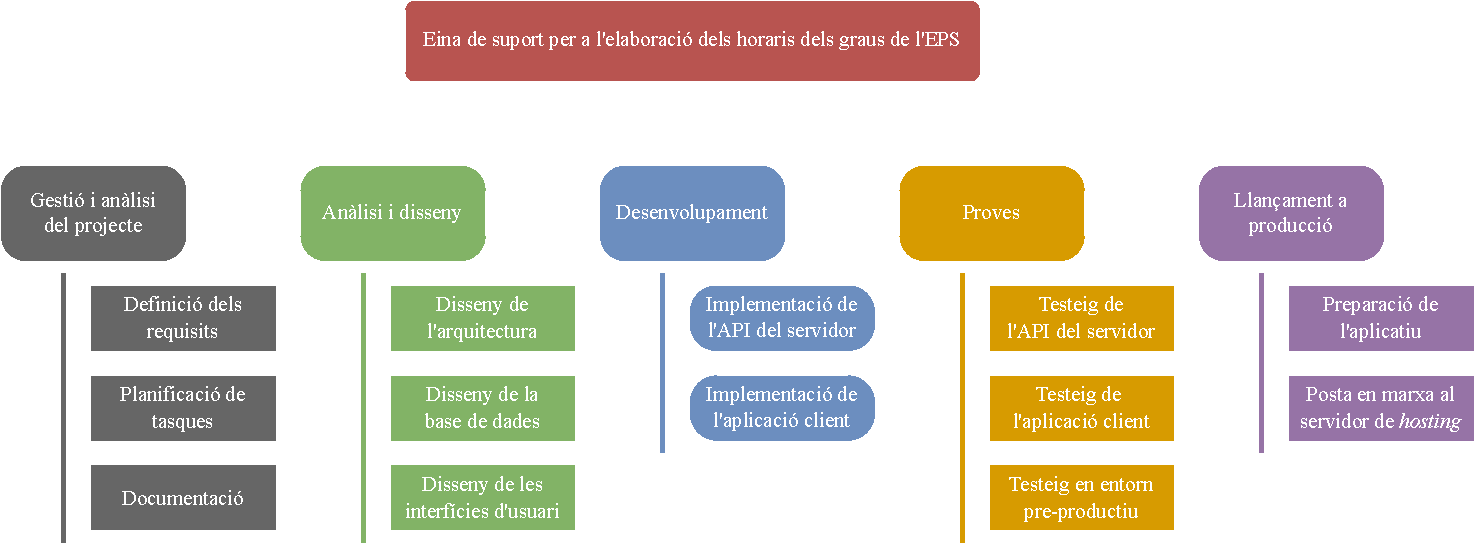
\includegraphics[width=\textwidth]{assets/working_packages/general.pdf}
	\caption{\label{img:pt_general}Descomposició general de les tasques del projecte.}
\end{figure}

\subsection{Gestió del projecte}
\label{subsec:gestio_projecte}

En aquesta subsecció, s'exposaran els paquets de treball que formen part de la branca de planificació \emph{Gestió del projecte}, la qual es pot tornar a veure a l'esquema següent:

\begin{figure}[H]
	\centering
	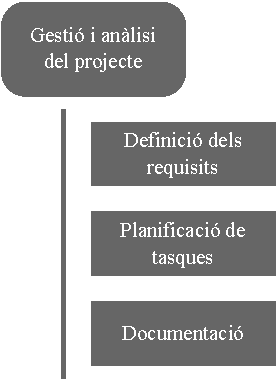
\includegraphics[width=0.35\textwidth]{assets/working_packages/gestioProjecte.pdf}
	\caption{\label{img:pt_gestio_projecte}Esquema de la branca de planificació \emph{Gestió del projecte}.}
\end{figure}

\begin{table}[H]
  \begin{tabularx}{\textwidth}{l | X}
    \toprule
    \rowcolor{Gray}
    \multicolumn{2}{c}{\texttt{\textbf{PT\_1.1:}} Definició dels requisits}\\
    \midrule[0.9pt]
    \textbf{Descripció}       & Anàlisi dels requisits que ha de complir l'aplicatiu del projecte.\\
    \midrule
    \textbf{Tasques}          & \textbf{T1:} Anàlisi i definició dels requisits no funcionals.
    \newline \textbf{T2:} Anàlisi i definició dels requisits de domini.
    \newline \textbf{T3:} Anàlisi i definició dels requisits funcionals.
    \newline \textbf{T4:} Confecció de la matriu de dependències entre els requisits.
    \newline \textbf{T5:} Verificació i comentari dels requisits amb els tutors.
    \newline \textbf{T6:} Correcció del document de requisits.\\
    \midrule
    \textbf{Temporalització}  & 45 hores.\\
    \midrule
    \textbf{Lliurable}        & Document de requisits del sistema (veure capítol~\ref{cap:requisits}).\\
    \bottomrule
  \end{tabularx}
  \caption{\label{taula:pt_1.1} Taula del paquet de treball \emph{Definició dels requisits}.}
\end{table}

\begin{table}[H]
  \begin{tabularx}{\textwidth}{l | X}
    \toprule
    \rowcolor{Gray}
    \multicolumn{2}{c}{\texttt{\textbf{PT\_1.2:}} Planificació de tasques}\\
    \midrule[0.9pt]
    \textbf{Descripció}       & Planificació de totes les tasques que involucra el projecte.\\
    \midrule
    \textbf{Tasques}          & \textbf{T1:} Descomposició i agrupació general de les tasques.
    \newline \textbf{T2:} Determinació i elaboració dels paquets de treball de cada grup de tasques.
    \newline \textbf{T3:} Confecció de la matriu de traçabilitat.
    \newline \textbf{T4:} Estimació del temps necessari per al desenvolupament del projecte i elaboració del cronograma.\\
    \midrule
    \textbf{Temporalització}  & 15 hores.\\
    \midrule
    \textbf{Lliurable}        & Documents de planificació i temporalització del projecte (veure capítol~\ref{cap:planificacio}).\\
    \bottomrule
  \end{tabularx}
  \caption{\label{taula:pt_1.2} Taula del paquet de treball \emph{Planificació de tasques}.}
\end{table}

\begin{table}[H]
  \begin{tabularx}{\textwidth}{l | X}
    \toprule
    \rowcolor{Gray}
    \multicolumn{2}{c}{\texttt{\textbf{PT\_1.3:}} Documentació}\\
    \midrule[0.9pt]
    \textbf{Descripció}       & Agrupació de la informació generada durant tot el procés de desenvolupament del projecte.\\
    \midrule
    \textbf{Tasques}          & \textbf{T1:} Redacció de la memòria del projecte.
    \newline \textbf{T2:} Verificació i comentari de la memòria amb els tutors.
    \newline \textbf{T3:} Correcció i retocament final de la memòria.\\
    \midrule
    \textbf{Temporalització}  & 60 hores.\\
    \midrule
    \textbf{Lliurable}        & Memòria del projecte.\\
    \bottomrule
  \end{tabularx}
  \caption{\label{taula:pt_1.3} Taula del paquet de treball \emph{Documentació}.}
\end{table}

\subsection{Anàlisi i disseny}
\label{subsec:analisi_disseny}

En aquesta subsecció, s'exposaran els paquets de treball que formen part de la branca de planificació \emph{Anàlisi i disseny}, la qual es pot tornar a veure a l'esquema següent:

\begin{figure}[htpb]
	\centering
	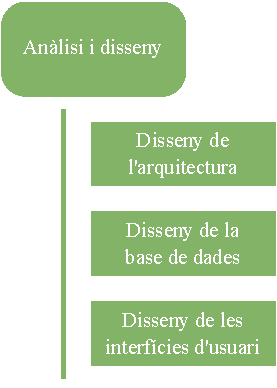
\includegraphics[width=0.35\textwidth]{assets/working_packages/analisiDisseny.pdf}
	\caption{\label{img:pt_analisi_disseny}Esquema de la branca de planificació \emph{Anàlisi i disseny}.}
\end{figure}

\begin{table}[H]
  \begin{tabularx}{\textwidth}{l | X}
    \toprule
    \rowcolor{Green}
    \multicolumn{2}{c}{\texttt{\textbf{PT\_2.1:}} Disseny de l'arquitectura}\\
    \midrule[0.9pt]
    \textbf{Descripció}       & Estudi i disseny de l'arquitectura de l'aplicatiu del projecte.\\
    \midrule
    \textbf{Tasques}          & \textbf{T1:} Estudi dels requisits.
    \newline \textbf{T2:} Estudi i decisió del tipus de base de dades que s'utilitzarà i del seu sistema gestor.
    \newline \textbf{T3:} Estudi i decisió del tipus de tecnologia amb la qual s'implementarà l'aplicació web client.
    \newline \textbf{T4:} Estudi i decisió del tipus de tecnologia amb la qual s'implementarà l'aplicació de l'API.\\
    \midrule
    \textbf{Temporalització}  & 10 hores.\\
    \midrule
    \textbf{Lliurable}        & Document de valoració i justificació de les tecnologies que conformen l'arquitectura de l'aplicatiu del projecte.\\
    \bottomrule
  \end{tabularx}
  \caption{\label{taula:pt_2.1} Taula del paquet de treball \emph{Disseny de l'arquitectura}.}
\end{table}

\begin{table}[H]
  \begin{tabularx}{\textwidth}{l | X}
    \toprule
    \rowcolor{Green}
    \multicolumn{2}{c}{\texttt{\textbf{PT\_2.2:}} Disseny de la base de dades}\\
    \midrule[0.9pt]
    \textbf{Descripció}       & Disseny de l'estructura de la base de dades de l'aplicatiu i determinació de la informació que s'hi emmagatzemarà.\\
    \midrule
    \textbf{Tasques}          & \textbf{T1:} Detall de les entitats que conformaran la base de dades.
    \newline \textbf{T2:} Decisió dels camps en què es dividiran les entitats, juntament amb el seu tipus i configuració.
    \newline \textbf{T3:} Determinació de les relacions que existiran entre les diferents entitats.
    \newline \textbf{T4:} Elaboració de l'esquema del model relacional.\\
    \midrule
    \textbf{Temporalització}  & 25 hores.\\
    \midrule
    \textbf{Lliurable}        & Esquema del model relacional de la base de dades.\\
    \bottomrule
  \end{tabularx}
  \caption{\label{taula:pt_2.2} Taula del paquet de treball \emph{Disseny de la base de dades}.}
\end{table}

\begin{table}[H]
  \begin{tabularx}{\textwidth}{l | X}
    \toprule
    \rowcolor{Green}
    \multicolumn{2}{c}{\texttt{\textbf{PT\_2.3:}} Disseny de les interfícies d'usuari}\\
    \midrule[0.9pt]
    \textbf{Descripció}       & Disseny de les interfícies d'usuari que es presentaran a l'aplicació web client.\\
    \midrule
    \textbf{Tasques}          & \textbf{T1:} Confecció dels esquemes de les interfícies d'usuari de les diferents parts de l'aplicació.
    \newline \textbf{T2:} Anàlisi dels esquemes i verificació de la seva adaptació als requisits.
    \newline \textbf{T3:} Plantejament de possibles nous requisits que hagin pogut sorgir a partir dels esquemes.\\
    \midrule
    \textbf{Temporalització}  & 85 hores.\\
    \midrule
    \textbf{Lliurable}        & Esquemes de les interfícies d'usuari de l'aplicació web client.\\
    \bottomrule
  \end{tabularx}
  \caption{\label{taula:pt_2.3} Taula del paquet de treball \emph{Disseny de les interfícies d'usuari}.}
\end{table}

\subsection{Desenvolupament}
\label{subsec:desenvolupament}

En aquesta subsecció, s'exposaran els paquets de treball que formen part de la branca de planificació \emph{Desenvolupament}, la qual es pot tornar a veure a l'esquema següent:

\begin{figure}[H]
	\centering
	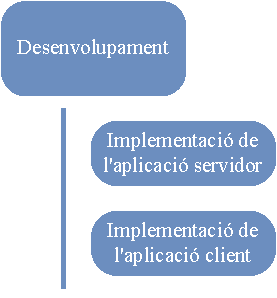
\includegraphics[width=0.35\textwidth]{assets/working_packages/desenvolupament/general.pdf}
	\caption{\label{img:pt_desenvolupament}Esquema de la branca de planificació \emph{Desenvolupament}.}
\end{figure}

A diferència de la resta de branques, aquesta no conté directament un conjunt de paquets de treball, sinó que en deriven altres branques. Als apartats següents es detallaran els paquets de treball que conté cadascuna.

\subsubsection{Implementació de l'API del servidor}
\label{subsubsec:implementacio_api}

\begin{figure}[H]
	\centering
	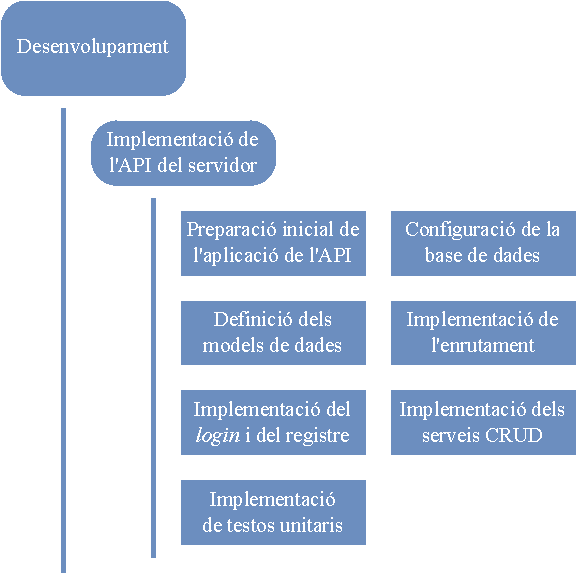
\includegraphics[width=0.7\textwidth]{assets/working_packages/desenvolupament/implementacioAPI.pdf}
	\caption{\label{img:pt_implementacio_api}Esquema de la branca de planificació derivada \emph{Implementació de l'API del servidor}.}
\end{figure}

\begin{table}[H]
  \begin{tabularx}{\textwidth}{l | X}
    \toprule
    \rowcolor{Blue}
    \multicolumn{2}{c}{\texttt{\textbf{PT\_3.1.1:}} Preparació inicial de l'aplicació de l'API}\\
    \midrule[0.9pt]
    \textbf{Descripció}       & Preparació i configuració inicial de l'aplicació de l'API del servidor.\\
    \midrule
    \textbf{Tasques}          & \textbf{T1:} Preparació de l'entorn de desenvolupament.
    \newline \textbf{T2:} Configuració del procés d'escolta de peticions.
    \newline \textbf{T3:} Implementació del tractament general de peticions i d'errors.
    \newline \textbf{T4:} Implementació del sistema de depuració i monitoreig.\\
    \midrule
    \textbf{Temporalització}  & 18 hores.\\
    \midrule
    \textbf{Lliurable}        & Aplicació de l'API del servidor preparada per ser implementada.\\
    \bottomrule
  \end{tabularx}
  \caption{\label{taula:pt_3.1.1} Taula del paquet de treball \emph{Preparació inicial de l'aplicació de l'API}.}
\end{table}

\begin{table}[H]
  \begin{tabularx}{\textwidth}{l | X}
    \toprule
    \rowcolor{Blue}
    \multicolumn{2}{c}{\texttt{\textbf{PT\_3.1.2:}} Configuració de la base de dades}\\
    \midrule[0.9pt]
    \textbf{Descripció}       & Configuració inicial del sistema gestor de la base de dades i de l'ORM (\textit{object relational mapper}).\\
    \midrule
    \textbf{Tasques}          & \textbf{T1:} Configuració de la connexió entre l'aplicació de l'API i el sistema gestor de la base de dades.
    \newline \textbf{T2:} Configuració de l'ORM escollit.
    \newline \textbf{T3:} Determinació dels usuaris del sistema gestor de la base de dades.\\
    \midrule
    \textbf{Temporalització}  & 5 hores.\\
    \midrule
    \textbf{Lliurable}        & Sistema gestor de la base de dades configurat.\\
    \bottomrule
  \end{tabularx}
  \caption{\label{taula:pt_3.1.2} Taula del paquet de treball \emph{Configuració de la base de dades}.}
\end{table}

\begin{table}[H]
  \begin{tabularx}{\textwidth}{l | X}
    \toprule
    \rowcolor{Blue}
    \multicolumn{2}{c}{\texttt{\textbf{PT\_3.1.3:}} Definició dels models de dades}\\
    \midrule[0.9pt]
    \textbf{Descripció}       & Definició dels models de dades que s'han de guardar a la base de dades.\\
    \midrule
    \textbf{Tasques}          & \textbf{T1:} Definició i configuració dels models de dades descrits a l'esquema del model relacional.
    \newline \textbf{T2:} Implementació de validadors de dades per a cada camp dels models.
    \newline \textbf{T3:} Implementació i configuració de les relacions entre models.\\
    \midrule
    \textbf{Temporalització}  & 20 hores.\\
    \midrule
    \textbf{Lliurable}        & Models de dades definits.\\
    \bottomrule
  \end{tabularx}
  \caption{\label{taula:pt_3.1.3} Taula del paquet de treball \emph{Definició dels models de dades}.}
\end{table}

\begin{table}[H]
  \begin{tabularx}{\textwidth}{l | X}
    \toprule
    \rowcolor{Blue}
    \multicolumn{2}{c}{\texttt{\textbf{PT\_3.1.4:}} Implementació de l'enrutament}\\
    \midrule[0.9pt]
    \textbf{Descripció}       & Definició dels diferents \textit{endpoints} de l'API i implementació de l'enrutament de peticions.\\
    \midrule
    \textbf{Tasques}          & \textbf{T1:} Definició dels \textit{endpoints} de l'API i de les seves rutes.
    \newline \textbf{T2:} Implementació de l'enrutament de peticions a l'\textit{endpoint} corresponent.
    \newline \textbf{T3:} Implementació dels mecanismes d'autorització segons el rol de l'usuari.\\
    \midrule
    \textbf{Temporalització}  & 20 hores.\\
    \midrule
    \textbf{Lliurable}        & Enrutament implementat.\\
    \bottomrule
  \end{tabularx}
  \caption{\label{taula:pt_3.1.4} Taula del paquet de treball \emph{Implementació de l'enrutament}.}
\end{table}

\begin{table}[H]
  \begin{tabularx}{\textwidth}{l | X}
    \toprule
    \rowcolor{Blue}
    \multicolumn{2}{c}{\texttt{\textbf{PT\_3.1.5:}} Implementació del \textit{login} i del registre}\\
    \midrule[0.9pt]
    \textbf{Descripció}       & Implementació del tractament de peticions d'autenticació i de registre d'usuaris.\\
    \midrule
    \textbf{Tasques}          & \textbf{T1:} Implementació inicial dels processos d'autenticació i de registre.
    \newline \textbf{T2:} Implementació dels mecanismes de seguretat involucrats.
    \newline \textbf{T3:} Implementació de l'enviament dels correus electrònics involucrats.\\
    \midrule
    \textbf{Temporalització}  & 20 hores.\\
    \midrule
    \textbf{Lliurable}        & \textit{Login} i registre implementats.\\
    \bottomrule
  \end{tabularx}
  \caption{\label{taula:pt_3.1.5} Taula del paquet de treball \emph{Implementació del \textit{login} i del registre}.}
\end{table}

\begin{table}[H]
  \begin{tabularx}{\textwidth}{l | X}
    \toprule
    \rowcolor{Blue}
    \multicolumn{2}{c}{\texttt{\textbf{PT\_3.1.6:}} Implementació dels serveis CRUD.}\\
    \midrule[0.9pt]
    \textbf{Descripció}       & Implementació dels serveis de creació, recuperació, modificació i eliminació per a cadascun dels models de dades.\\
    \midrule
    \textbf{Tasques}          & \textbf{T1:} Implementació dels serveis CRUD per als models de dades relacionats amb els Administradors.
    \newline \textbf{T2:} Implementació dels serveis CRUD per als models de dades relacionats amb els Coordinadors.
    \newline \textbf{T3:} Implementació dels serveis CRUD per als models de dades relacionats amb els Directors de departament.
    \newline \textbf{T4:} Implementació dels serveis CRUD per als models de dades relacionats amb els Responsables de docència.
    \newline \textbf{T5:} Implementació dels serveis CRUD per als models de dades relacionats amb els Professors.\\
    \midrule
    \textbf{Temporalització}  & 85 hores.\\
    \midrule
    \textbf{Lliurable}        & Serveis de CRUD implementats.\\
    \bottomrule
  \end{tabularx}
  \caption{\label{taula:pt_3.1.6} Taula del paquet de treball \emph{Implementació dels serveis CRUD.}}
\end{table}

\begin{table}[H]
  \begin{tabularx}{\textwidth}{l | X}
    \toprule
    \rowcolor{Blue}
    \multicolumn{2}{c}{\texttt{\textbf{PT\_3.1.7:}} Implementació de testos unitaris}\\
    \midrule[0.9pt]
    \textbf{Descripció}       & Disseny i implementació de testos unitaris per als diferents procediments de l'aplicació de l'API del servidor.\\
    \midrule
    \textbf{Tasques}          & \textbf{T1:} Disseny, implementació i execució continuades de testos unitaris.\\
    \midrule
    \textbf{Temporalització}  & 10 hores.\\
    \midrule
    \textbf{Lliurable}        & Testos implementats.\\
    \bottomrule
  \end{tabularx}
  \caption{\label{taula:pt_3.1.7} Taula del paquet de treball \emph{Implementació de testos unitaris}.}
\end{table}


\subsubsection{Implementació del client}
\label{subsubsec:implementacio_client}

\begin{figure}[H]
	\centering
	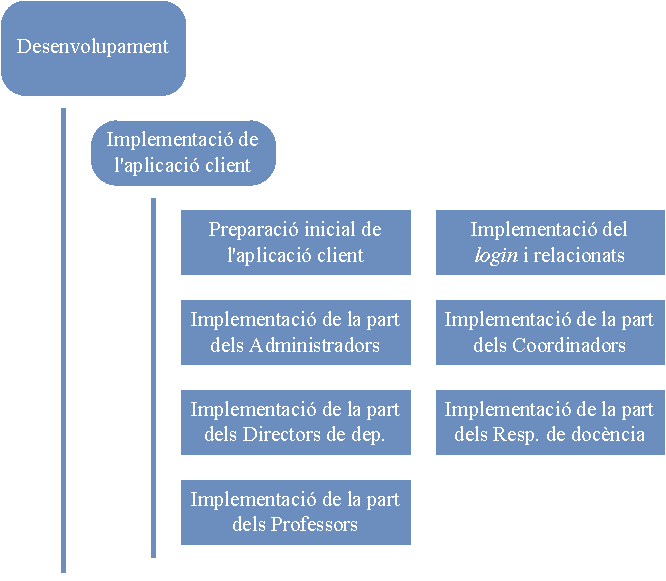
\includegraphics[width=0.7\textwidth]{assets/working_packages/desenvolupament/implementacioClient.pdf}
	\caption{\label{img:pt_implementacio_client}Esquema de la branca de planificació derivada \emph{Implementació del client}.}
\end{figure}

\begin{table}[H]
  \begin{tabularx}{\textwidth}{l | X}
    \toprule
    \rowcolor{Blue}
    \multicolumn{2}{c}{\texttt{\textbf{PT\_3.2.1:}} Preparació inicial de l'aplicació client}\\
    \midrule[0.9pt]
    \textbf{Descripció}       & Preparació i configuració inicial de l'aplicació client.\\
    \midrule
    \textbf{Tasques}          & \textbf{T1:} Preparació de l'entorn de desenvolupament.\\
    \midrule
    \textbf{Temporalització}  & 9 hores.\\
    \midrule
    \textbf{Lliurable}        & Aplicació client preparada per ser implementada.\\
    \bottomrule
  \end{tabularx}
  \caption{\label{taula:pt_3.2.1} Taula del paquet de treball \emph{Preparació inicial de l'aplicació client}.}
\end{table}

\begin{table}[H]
  \begin{tabularx}{\textwidth}{l | X}
    \toprule
    \rowcolor{Blue}
    \multicolumn{2}{c}{\texttt{\textbf{PT\_3.2.2:}} Implementació del \textit{login} i relacionats.}\\
    \midrule[0.9pt]
    \textbf{Descripció}       & Implementació de les finestres i procediments relacionats amb l'autenticació dels usuaris.\\
    \midrule
    \textbf{Tasques}          & \textbf{T1:} Implementació de la finestra d'autenticació.
    \newline \textbf{T2:} Implementació del conjunt de finestres de restabliment de contrasenya.\\
    \midrule
    \textbf{Temporalització}  & 30 hores.\\
    \midrule
    \textbf{Lliurable}        & Finestres i procediments de \textit{login} i relacionats implementats.\\
    \bottomrule
  \end{tabularx}
  \caption{\label{taula:pt_3.2.2} Taula del paquet de treball \emph{Implementació del \textit{login} i relacionats}.}
\end{table}

\begin{table}[H]
  \begin{tabularx}{\textwidth}{l | X}
    \toprule
    \rowcolor{Blue}
    \multicolumn{2}{c}{\texttt{\textbf{PT\_3.2.3:}} Implementació de la part dels Administradors}\\
    \midrule[0.9pt]
    \textbf{Descripció}       & Implementació de les finestres i procediments que involucren els usuaris amb rol d'Administrador.\\
    \midrule
    \textbf{Tasques}          & \textbf{T1:} Implementació del conjunt de finestres relacionades amb la gestió de plans docents.
    \newline \textbf{T2:} Implementació del conjunt de finestres relacionades amb l'assignació d'aules.
    \newline \textbf{T3:} Implementació del conjunt de finestres relacionades amb la gestió de Coordinadors.
    \newline \textbf{T4:} Implementació del conjunt de finestres relacionades amb la gestió de Directors de departament.\\
    \midrule
    \textbf{Temporalització}  & 45 hores.\\
    \midrule
    \textbf{Lliurable}        & Part dels usuaris Administradors implementada.\\
    \bottomrule
  \end{tabularx}
  \caption{\label{taula:pt_3.2.3} Taula del paquet de treball \emph{Implementació de la part dels Administradors}.}
\end{table}

\begin{table}[H]
  \begin{tabularx}{\textwidth}{l | X}
    \toprule
    \rowcolor{Blue}
    \multicolumn{2}{c}{\texttt{\textbf{PT\_3.2.4:}} Implementació de la part dels Coordinadors}\\
    \midrule[0.9pt]
    \textbf{Descripció}       & Implementació de les finestres i procediments que involucren els usuaris amb rol de Coordinador.\\
    \midrule
    \textbf{Tasques}          & \textbf{T1:} Implementació del conjunt de finestres relacionades amb la gestió d'horaris de graus.
    \newline \textbf{T2:} Implementació del conjunt de finestres relacionades amb la consulta d'horaris de Professors.
    \newline \textbf{T3:} Implementació del conjunt de finestres relacionades amb la consulta d'horaris d'aules.\\
    \midrule
    \textbf{Temporalització}  & 50 hores.\\
    \midrule
    \textbf{Lliurable}        & Part dels usuaris Coordinadors implementada.\\
    \bottomrule
  \end{tabularx}
  \caption{\label{taula:pt_3.2.4} Taula del paquet de treball \emph{Implementació de la part dels Coordinadors}.}
\end{table}

\begin{table}[H]
  \begin{tabularx}{\textwidth}{l | X}
    \toprule
    \rowcolor{Blue}
    \multicolumn{2}{c}{\texttt{\textbf{PT\_3.2.5:}} Implementació de la part dels Directors de departament}\\
    \midrule[0.9pt]
    \textbf{Descripció}       & Implementació de les finestres i procediments que involucren els usuaris amb rol de Director de departament.\\
    \midrule
    \textbf{Tasques}          & \textbf{T1:} Implementació del conjunt de finestres relacionades amb la consulta d'horaris de Professors.
    \newline \textbf{T2:} Implementació del conjunt de finestres relacionades amb la consulta d'horaris de graus.
    \newline \textbf{T3:} Implementació del conjunt de finestres relacionades amb la gestió de Responsables de docència.\\
    \midrule
    \textbf{Temporalització}  & 15 hores.\\
    \midrule
    \textbf{Lliurable}        & Part dels usuaris Directors de departament implementada.\\
    \bottomrule
  \end{tabularx}
  \caption{\label{taula:pt_3.2.5} Taula del paquet de treball \emph{Implementació de la part dels Directors de departament}.}
\end{table}

\begin{table}[H]
  \begin{tabularx}{\textwidth}{l | X}
    \toprule
    \rowcolor{Blue}
    \multicolumn{2}{c}{\texttt{\textbf{PT\_3.2.6:}} Implementació de la part dels Responsables de docència}\\
    \midrule[0.9pt]
    \textbf{Descripció}       & Implementació de les finestres i procediments que involucren els usuaris amb rol de Responsable de docència.\\
    \midrule
    \textbf{Tasques}          & \textbf{T1:} Implementació del conjunt de finestres relacionades amb la consulta d'horaris de Professors.
    \newline \textbf{T2:} Implementació del conjunt de finestres relacionades amb l'assignació de Professors.
    \newline \textbf{T3:} Implementació del conjunt de finestres relacionades amb la gestió de Professors.\\
    \midrule
    \textbf{Temporalització}  & 25 hores.\\
    \midrule
    \textbf{Lliurable}        & Part dels usuaris Responsables de docència implementada.\\
    \bottomrule
  \end{tabularx}
  \caption{\label{taula:pt_3.2.6} Taula del paquet de treball \emph{Implementació de la part dels Responsables de docència}.}
\end{table}

\begin{table}[H]
  \begin{tabularx}{\textwidth}{l | X}
    \toprule
    \rowcolor{Blue}
    \multicolumn{2}{c}{\texttt{\textbf{PT\_3.2.7:}} Implementació de la part dels Professors}\\
    \midrule[0.9pt]
    \textbf{Descripció}       & Implementació de les finestres i procediments que involucren els usuaris amb rol de Professor.\\
    \midrule
    \textbf{Tasques}          & \textbf{T1:} Implementació del conjunt de finestres relacionades amb la consulta dels propis horaris.
    \newline \textbf{T2:} Implementació del conjunt de finestres relacionades amb la consulta d'horaris d'assignatures.
    \newline \textbf{T3:} Implementació del conjunt de finestres relacionades amb la consulta d'horaris de graus.\\
    \midrule
    \textbf{Temporalització}  & 15 hores.\\
    \midrule
    \textbf{Lliurable}        & Part dels usuaris Professors implementada.\\
    \bottomrule
  \end{tabularx}
  \caption{\label{taula:pt_3.2.7} Taula del paquet de treball \emph{Implementació de la part dels Professors}.}
\end{table}


\subsection{Proves}
\label{subsec:proves}

En aquesta subsecció, s'exposaran els paquets de treball que formen part de la branca de planificació \emph{Proves}, la qual es pot tornar a veure a l'esquema següent:

\begin{figure}[htpb]
	\centering
	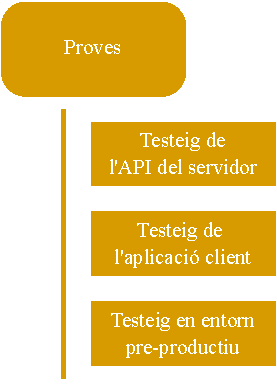
\includegraphics[width=0.35\textwidth]{assets/working_packages/proves.pdf}
	\caption{\label{img:pt_proves}Esquema de la branca de planificació \emph{Proves}.}
\end{figure}

\begin{table}[H]
  \begin{tabularx}{\textwidth}{l | X}
    \toprule
    \rowcolor{Orange}
    \multicolumn{2}{c}{\texttt{\textbf{PT\_4.1:}} Testeig de l'API del servidor}\\
    \midrule[0.9pt]
    \textbf{Descripció}       & Realització de proves i depuració de l'API del servidor.\\
    \midrule
    \textbf{Tasques}          & \textbf{T1:} Disseny de les proves que s'han de realitzar.
    \newline \textbf{T2:} Efectuació de les proves i anàlisi dels resultats.
    \newline \textbf{T3:} Correcció dels errors que hagin pogut aparèixer.\\
    \midrule
    \textbf{Temporalització}  & 5 hores.\\
    \midrule
    \textbf{Lliurable}        & Proves i depuració de l'API del servidor realitzada.\\
    \bottomrule
  \end{tabularx}
  \caption{\label{taula:pt_4.1} Taula del paquet de treball \emph{Testeig de l'API del servidor}.}
\end{table}

\begin{table}[H]
  \begin{tabularx}{\textwidth}{l | X}
    \toprule
    \rowcolor{Orange}
    \multicolumn{2}{c}{\texttt{\textbf{PT\_4.2:}} Testeig de l'aplicació client}\\
    \midrule[0.9pt]
    \textbf{Descripció}       & Realització de proves i depuració de l'aplicació client.\\
    \midrule
    \textbf{Tasques}          & \textbf{T1:} Disseny de les proves que s'han de realitzar.
    \newline \textbf{T2:} Efectuació de les proves i anàlisi dels resultats.
    \newline \textbf{T3:} Correcció dels errors que hagin pogut aparèixer.\\
    \midrule
    \textbf{Temporalització}  & 20 hores.\\
    \midrule
    \textbf{Lliurable}        & Proves i depuració de l'aplicació client realitzada.\\
    \bottomrule
  \end{tabularx}
  \caption{\label{taula:pt_4.2} Taula del paquet de treball \emph{Testeig de l'aplicació client}.}
\end{table}

\begin{table}[H]
  \begin{tabularx}{\textwidth}{l | X}
    \toprule
    \rowcolor{Orange}
    \multicolumn{2}{c}{\texttt{\textbf{PT\_4.3:}} Testeig en entorn preproductiu}\\
    \midrule[0.9pt]
    \textbf{Descripció}       & Realització de proves i depuració en un entorn igual que el productiu.\\
    \midrule
    \textbf{Tasques}          & \textbf{T1:} Simulació de situacions reals a mode de prova.
    \newline \textbf{T2:} Simulació de situacions reals a mode de prova pels usuaris finals.
    \newline \textbf{T3:} Correcció dels errors que hagin pogut aparèixer.\\
    \midrule
    \textbf{Temporalització}  & 10 hores.\\
    \midrule
    \textbf{Lliurable}        & Proves i depuració en un entorn pre-productiu realitzada.\\
    \bottomrule
  \end{tabularx}
  \caption{\label{taula:pt_4.3} Taula del paquet de treball \emph{Testeig en entorn preproductiu}.}
\end{table}


\subsection{Llançament a producció}
\label{subsec:llancament_produccio}

En aquesta subsecció, s'exposaran els paquets de treball que formen part de la branca de planificació \emph{Llançament a producció}, la qual es pot tornar a veure a l'esquema següent:

\begin{figure}[htpb]
	\centering
	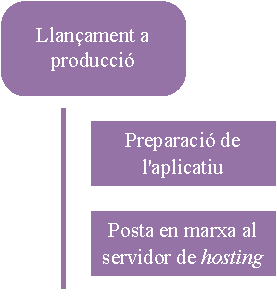
\includegraphics[width=0.35\textwidth]{assets/working_packages/llancamentProduccio.pdf}
	\caption{\label{img:pt_llancament_roduccio}Esquema de la branca de planificació \emph{Llançament a producció}.}
\end{figure}

\begin{table}[H]
  \begin{tabularx}{\textwidth}{l | X}
    \toprule
    \rowcolor{Purple}
    \multicolumn{2}{c}{\texttt{\textbf{PT\_6.1:}} Preparació de l'aplicatiu}\\
    \midrule[0.9pt]
    \textbf{Descripció}       & Preparació de l'aplicatiu per al llançament a producció.\\
    \midrule
    \textbf{Tasques}          & \textbf{T1:} Revisió i neteja del codi font.
    \newline \textbf{T2:} Verificació que no es mostra cap informació en pantalla o en consola que pugui comprometre la seguretat.
    \newline \textbf{T3:} Comprovació que les variables d'entorn es recuperen correctament.
    \newline \textbf{T4:} Altres poliments.\\
    \midrule
    \textbf{Temporalització}  & 4 hores.\\
    \midrule
    \textbf{Lliurable}        & Aplicatiu preparat per al llançament a producció.\\
    \bottomrule
  \end{tabularx}
  \caption{\label{taula:pt_6.1} Taula del paquet de treball \emph{Preparació de l'aplicatiu}.}
\end{table}

\begin{table}[H]
  \begin{tabularx}{\textwidth}{l | X}
    \toprule
    \rowcolor{Purple}
    \multicolumn{2}{c}{\texttt{\textbf{PT\_6.2:}} Posada en marxa al servidor de \textit{hosting}}\\
    \midrule[0.9pt]
    \textbf{Descripció}       & Llançament a producció de l'aplicatiu al servidor de \textit{hosting}.\\
    \midrule
    \textbf{Tasques}          & \textbf{T1:} Configuració general del servidor.
    \newline \textbf{T2:} Traspàs de l'aplicatiu al servidor.
    \newline \textbf{T3:} Establiment de les variables d'entorn corresponents.
    \newline \textbf{T4:} Posada en marxa de l'aplicatiu i realització de comprovacions.\\
    \midrule
    \textbf{Temporalització}  & 8 hores.\\
    \midrule
    \textbf{Lliurable}        & Aplicatiu en funcionament a l'entorn productiu.\\
    \bottomrule
  \end{tabularx}
  \caption{\label{taula:pt_6.2} Taula del paquet de treball \emph{Posada en marxa al servidor de \textit{hosting}}.}
\end{table}


\section{Matriu de traçabilitat}
\label{sec:matriu_tracabilitat}

En aquesta secció, es representarà la matriu de traçabilitat que relaciona els paquets de treball definits a la secció anterior i els requisits (veure capítol~\ref{cap:requisits}).

D'aquesta manera, es podrà saber quins requisits s'assoleixen un cop completades les tasques dels paquets de treball.

El format que adoptarà cadascuna de les relacions es defineix a continuació:
\\[8pt]
\centerline{(\texttt{\textbf{RF-X}, \texttt{\textbf{RF-Y}}}, \texttt{\textbf{\ldots}}) $\longrightarrow$ (\texttt{\textbf{PT\_P}}, \texttt{\textbf{PT\_Q}, \texttt{\textbf{\ldots}}})}

És a dir, la llista de requisits de la part anterior de la flexta s'assoleix un cop completada la de paquets de treball situada a la part posterior.

La matriu de traçabilitat completa és la següent:
\begin{itemize}
  \item (\texttt{\textbf{RF-G1}}, \texttt{\textbf{RF-G3}}) \hspace{1pt} $\longrightarrow$ \hspace{1pt} (\texttt{\textbf{PT\_3.1.5}}, \texttt{\textbf{PT\_3.2.2}})
  \item (\texttt{\textbf{RF-G2}}) \hspace{1pt} $\longrightarrow$ \hspace{1pt} (\texttt{\textbf{PT\_3.1.5}}, \texttt{\textbf{PT\_3.2.3}}, \texttt{\textbf{PT\_3.2.5}}, \texttt{\textbf{PT\_3.2.6}})
  \item (\texttt{\textbf{RF-G4}}, \texttt{\textbf{RF-G6}}, \texttt{\textbf{RF-G7}}, \texttt{\textbf{RF-G8}}) \hspace{1pt} $\longrightarrow$ \hspace{1pt} (\texttt{\textbf{PT\_3.1.6}}, \texttt{\textbf{PT\_3.2.3}}, \texttt{\textbf{PT\_3.2.4}}, \texttt{\textbf{PT\_3.2.5}}, \texttt{\textbf{PT\_3.2.6}}, \texttt{\textbf{PT\_3.2.7}})
  \item (\texttt{\textbf{RF-G5}}) \hspace{1pt} $\longrightarrow$ \hspace{1pt} (\texttt{\textbf{PT\_3.1.4}})
  \item (\texttt{\textbf{RF-G9}}) \hspace{1pt} $\longrightarrow$ \hspace{1pt} (\texttt{\textbf{PT\_2.2}}, \texttt{\textbf{PT\_3.1.2}}, \texttt{\textbf{PT\_3.1.3}})
  \item (\texttt{\textbf{RF-G10}}) \hspace{1pt} $\longrightarrow$ \hspace{1pt} (\texttt{\textbf{PT\_3.1.2}}, \texttt{\textbf{PT\_3.2.3}})
  \item (\texttt{\textbf{RF-A1}}, \texttt{\textbf{RF-A2}}, \texttt{\textbf{RF-A3}}, \texttt{\textbf{RF-A4}}, \texttt{\textbf{RF-A5}}, \texttt{\textbf{RF-A6}}, \texttt{\textbf{RF-A7}}, \texttt{\textbf{RF-A8}}, \texttt{\textbf{RF-A9}}, \texttt{\textbf{RF-A10}}, \texttt{\textbf{RF-A11}}, \texttt{\textbf{RF-A13}}, \texttt{\textbf{RF-A14}}, \texttt{\textbf{RF-A15}}, \texttt{\textbf{RF-A16}}, \texttt{\textbf{RF-A17}}, \texttt{\textbf{RF-A18}}, \texttt{\textbf{RF-A20}}) \hspace{1pt} $\longrightarrow$ \hspace{1pt} (\texttt{\textbf{PT\_3.1.6}}, \texttt{\textbf{PT\_3.2.3}})
  \item (\texttt{\textbf{RF-A12}}, \texttt{\textbf{RF-A19}}) \hspace{1pt} $\longrightarrow$ \hspace{1pt} (\texttt{\textbf{PT\_3.1.5}}, \texttt{\textbf{PT\_3.1.6}}, \texttt{\textbf{PT\_3.2.3}})
  \item (\texttt{\textbf{RF-C1}}, \texttt{\textbf{RF-C2}}, \texttt{\textbf{RF-C3}}, \texttt{\textbf{RF-C4}}, \texttt{\textbf{RF-C5}}, \texttt{\textbf{RF-C6}}, \texttt{\textbf{RF-C7}}, \texttt{\textbf{RF-C8}}, \texttt{\textbf{RF-C9}}) \hspace{1pt} $\longrightarrow$ \hspace{1pt} (\texttt{\textbf{PT\_3.1.6}}, \texttt{\textbf{PT\_3.2.4}})
  \item (\texttt{\textbf{RF-D1}}, \texttt{\textbf{RF-D2}}, \texttt{\textbf{RF-D3}}, \texttt{\textbf{RF-D4}}, \texttt{\textbf{RF-D5}}, \texttt{\textbf{RF-D6}}, \texttt{\textbf{RF-D7}}, \texttt{\textbf{RF-D9}}) \hspace{1pt} $\longrightarrow$ \hspace{1pt} (\texttt{\textbf{PT\_3.1.6}}, \texttt{\textbf{PT\_3.2.5}})
  \item (\texttt{\textbf{RF-D8}}) \hspace{1pt} $\longrightarrow$ \hspace{1pt} (\texttt{\textbf{PT\_3.1.5}}, \texttt{\textbf{PT\_3.1.6}}, \texttt{\textbf{PT\_3.2.5}})
  \item (\texttt{\textbf{RF-R1}}, \texttt{\textbf{RF-R2}}, \texttt{\textbf{RF-R3}}, \texttt{\textbf{RF-R4}}, \texttt{\textbf{RF-R6}}) \hspace{1pt} $\longrightarrow$ \hspace{1pt} (\texttt{\textbf{PT\_3.1.6}}, \texttt{\textbf{PT\_3.2.6}})
  \item (\texttt{\textbf{RF-R5}}, \texttt{\textbf{RF-G3}}) \hspace{1pt} $\longrightarrow$ \hspace{1pt} (\texttt{\textbf{PT\_3.1.5}}, \texttt{\textbf{PT\_3.1.6}}, \texttt{\textbf{PT\_3.2.6}})
  \item (\texttt{\textbf{RF-P1}}, \texttt{\textbf{RF-P2}}, \texttt{\textbf{RF-P3}}) \hspace{1pt} $\longrightarrow$ \hspace{1pt} (\texttt{\textbf{PT\_3.1.6}}, \texttt{\textbf{PT\_3.2.7}})
\end{itemize}

\section{Temporalització}
\label{sec:temporalitzacio}

\subsection{Determinació d'activitats}
\label{subsec:determinacio_activitats}

En aquesta subsecció, a partir de la matriu de dependències (veure secció~\ref{sec:matriu_dependencies}) i la de traçabilitat (veure secció~\ref{sec:matriu_tracabilitat}), es determinaran les activitats que caldrà dur a terme per completar el desenvolupament del projecte.

Una activitat és una agrupació de paquets de treball i/o de tasques de paquets de treball que cal completar per poder assolir una sèrie de requisits.

Un cop s'hagin determinat les activitats, s'efectuarà una estimació del temps que podria requerir completar cadascuna. Aquesta estimació consistirà, primerament, en indicar tres valors de temps:

\begin{itemize}
  \item \textit{t(O)}: Estimació optimista.
  \item \textit{t(M)}: El més probable.
  \item \textit{t(P)}: Estimació pessimista.
\end{itemize}

Tot seguit, es calcularà el temps esperat de duració \textit{t(E)} de l'activitat. Aquest càlcul consisteix en una mitjana ponderada dels valors de l'estimació anterior, tal com es pot veure a continuació:

\begin{equation}
  t(E) = \frac{t(O) + 4t(M) + t(P)}{6}
\end{equation}

\begin{table}[H]
  \begin{tabularx}{\textwidth}{l | X}
    \toprule
    \rowcolor{Gray}
    \multicolumn{2}{c}{\texttt{\textbf{A1:}} Definició de requisits}\\
    \midrule[0.9pt]
    \textbf{Tasques}                 & \texttt{\textbf{PT\_1.1}}.\\
    \midrule
    \textbf{Estimació de temps}      & \textit{t(O)}: 20 hores.
    \newline \textit{t(M)}: 30 hores.
    \newline \textit{t(P)}: 45 hores.\\
    \midrule
    \textbf{Durada esperada}         & \textbf{\textit{t(E)}: 31 hores}.\\
    \bottomrule
  \end{tabularx}
  \caption{\label{taula:a1} Taula de l'activitat \emph{Definició de requisits}.}
\end{table}

\begin{table}[H]
  \begin{tabularx}{\textwidth}{l | X}
    \toprule
    \rowcolor{Gray}
    \multicolumn{2}{c}{\texttt{\textbf{A2:}} Planificació de tasques}\\
    \midrule[0.9pt]
    \textbf{Tasques}                 & \texttt{\textbf{PT\_1.2}}.\\
    \midrule
    \textbf{Estimació de temps}      & \textit{t(O)}: 10 hores.
    \newline \textit{t(M)}: 15 hores.
    \newline \textit{t(P)}: 25 hores.\\
    \midrule
    \textbf{Durada esperada}         & \textbf{\textit{t(E)}: 16 hores}.\\
    \bottomrule
  \end{tabularx}
  \caption{\label{taula:a2} Taula de l'activitat \emph{Planificació de tasques}.}
\end{table}

\begin{table}[H]
  \begin{tabularx}{\textwidth}{l | X}
    \toprule
    \rowcolor{Green}
    \multicolumn{2}{c}{\texttt{\textbf{A3:}} Disseny de l'arquitectura}\\
    \midrule[0.9pt]
    \textbf{Tasques}                 & \texttt{\textbf{PT\_2.1}}.\\
    \midrule
    \textbf{Estimació de temps}      & \textit{t(O)}: 6 hores.
    \newline \textit{t(M)}: 10 hores.
    \newline \textit{t(P)}: 20 hores.\\
    \midrule
    \textbf{Durada esperada}         & \textbf{\textit{t(E)}: 11 hores}.\\
    \bottomrule
  \end{tabularx}
  \caption{\label{taula:a3} Taula de l'activitat \emph{Disseny de l'arquitectura}.}
\end{table}

\begin{table}[H]
  \begin{tabularx}{\textwidth}{l | X}
    \toprule
    \rowcolor{Green}
    \multicolumn{2}{c}{\texttt{\textbf{A4:}} Disseny de la base de dades}\\
    \midrule[0.9pt]
    \textbf{Tasques}                 & \texttt{\textbf{PT\_2.2}}.\\
    \midrule
    \textbf{Estimació de temps}      & \textit{t(O)}: 15 hores.
    \newline \textit{t(M)}: 25 hores.
    \newline \textit{t(P)}: 30 hores.\\
    \midrule
    \textbf{Durada esperada}         & \textbf{\textit{t(E)}: 24 hores}.\\
    \bottomrule
  \end{tabularx}
  \caption{\label{taula:a4} Taula de l'activitat \emph{Disseny de la base de dades}.}
\end{table}

\begin{table}[H]
  \begin{tabularx}{\textwidth}{l | X}
    \toprule
    \rowcolor{Green}
    \multicolumn{2}{c}{\texttt{\textbf{A5:}} Disseny de les interfícies d'usuari}\\
    \midrule[0.9pt]
    \textbf{Tasques}                 & \texttt{\textbf{PT\_2.3}}.\\
    \midrule
    \textbf{Estimació de temps}      & \textit{t(O)}: 60 hores.
    \newline \textit{t(M)}: 85 hores.
    \newline \textit{t(P)}: 120 hores.\\
    \midrule
    \textbf{Durada esperada}         & \textbf{\textit{t(E)}: 87 hores}.\\
    \bottomrule
  \end{tabularx}
  \caption{\label{taula:a5} Taula de l'activitat \emph{Disseny de les interfícies d'usuari}.}
\end{table}

\begin{table}[H]
  \begin{tabularx}{\textwidth}{l | X}
    \toprule
    \rowcolor{Blue}
    \multicolumn{2}{c}{\texttt{\textbf{A6:}} Preparació inicial de l'aplicació de l'API}\\
    \midrule[0.9pt]
    \textbf{Tasques}                 & \texttt{\textbf{PT\_3.1.1}}.\\
    \midrule
    \textbf{Estimació de temps}      & \textit{t(O)}: 12 hores.
    \newline \textit{t(M)}: 18 hores.
    \newline \textit{t(P)}: 28 hores.\\
    \midrule
    \textbf{Durada esperada}         & \textbf{\textit{t(E)}: 19 hores}.\\
    \bottomrule
  \end{tabularx}
  \caption{\label{taula:a6} Taula de l'activitat \emph{Preparació inicial de l'aplicació de l'API}.}
\end{table}

\begin{table}[H]
  \begin{tabularx}{\textwidth}{l | X}
    \toprule
    \rowcolor{Blue}
    \multicolumn{2}{c}{\texttt{\textbf{A7:}} Configuració de la base de dades}\\
    \midrule[0.9pt]
    \textbf{Tasques}                 & \texttt{\textbf{PT\_3.1.2}}.\\
    \midrule
    \textbf{Estimació de temps}      & \textit{t(O)}: 3 hores.
    \newline \textit{t(M)}: 5 hores.
    \newline \textit{t(P)}: 10 hores.\\
    \midrule
    \textbf{Durada esperada}         & \textbf{\textit{t(E)}: 6 hores}.\\
    \bottomrule
  \end{tabularx}
  \caption{\label{taula:a7} Taula de l'activitat \emph{Configuració de la base de dades}.}
\end{table}

\begin{table}[H]
  \begin{tabularx}{\textwidth}{l | X}
    \toprule
    \rowcolor{Blue}
    \multicolumn{2}{c}{\texttt{\textbf{A8:}} Definició dels models de dades}\\
    \midrule[0.9pt]
    \textbf{Tasques}                 & \texttt{\textbf{PT\_3.1.3}}.\\
    \midrule
    \textbf{Estimació de temps}      & \textit{t(O)}: 18 hores.
    \newline \textit{t(M)}: 20 hores.
    \newline \textit{t(P)}: 30 hores.\\
    \midrule
    \textbf{Durada esperada}         & \textbf{\textit{t(E)}: 21 hores}.\\
    \bottomrule
  \end{tabularx}
  \caption{\label{taula:a8} Taula de l'activitat \emph{Definició dels models de dades}.}
\end{table}

\begin{table}[H]
  \begin{tabularx}{\textwidth}{l | X}
    \toprule
    \rowcolor{Blue}
    \multicolumn{2}{c}{\texttt{\textbf{A9:}} Implementació de l'enrutament}\\
    \midrule[0.9pt]
    \textbf{Tasques}                 & \texttt{\textbf{PT\_3.1.4}}.\\
    \midrule
    \textbf{Estimació de temps}      & \textit{t(O)}: 15 hores.
    \newline \textit{t(M)}: 20 hores.
    \newline \textit{t(P)}: 25 hores.\\
    \midrule
    \textbf{Durada esperada}         & \textbf{\textit{t(E)}: 25 hores}.\\
    \bottomrule
  \end{tabularx}
  \caption{\label{taula:a9} Taula de l'activitat \emph{Implementació de l'enrutament}.}
\end{table}

\begin{table}[H]
  \begin{tabularx}{\textwidth}{l | X}
    \toprule
    \rowcolor{Blue}
    \multicolumn{2}{c}{\texttt{\textbf{A10:}} Preparació inicial de l'aplicació client}\\
    \midrule[0.9pt]
    \textbf{Tasques}                 & \texttt{\textbf{PT\_3.2.1}}.\\
    \midrule
    \textbf{Estimació de temps}      & \textit{t(O)}: 6 hores.
    \newline \textit{t(M)}: 8 hores.
    \newline \textit{t(P)}: 15 hores.\\
    \midrule
    \textbf{Durada esperada}         & \textbf{\textit{t(E)}: 9 hores}.\\
    \bottomrule
  \end{tabularx}
  \caption{\label{taula:a10} Taula de l'activitat \emph{Preparació inicial de l'aplicació client}.}
\end{table}

\begin{table}[H]
  \begin{tabularx}{\textwidth}{l | X}
    \toprule
    \rowcolor{Blue}
    \multicolumn{2}{c}{\texttt{\textbf{A11:}} Implementació del \textit{login} i relacionats}\\
    \midrule[0.9pt]
    \textbf{Tasques}                 & \texttt{\textbf{PT\_3.1.5}}, \texttt{\textbf{PT\_3.2.2}}.\\
    \midrule
    \textbf{Estimació de temps}      & \textit{t(O)}: 25 hores.
    \newline \textit{t(M)}: 35 hores.
    \newline \textit{t(P)}: 50 hores.\\
    \midrule
    \textbf{Durada esperada}         & \textbf{\textit{t(E)}: 36 hores}.\\
    \bottomrule
  \end{tabularx}
  \caption{\label{taula:a11} Taula de l'activitat \emph{Implementació del \textit{login} i relacionats}.}
\end{table}

\begin{table}[H]
  \begin{tabularx}{\textwidth}{l | X}
    \toprule
    \rowcolor{Blue}
    \multicolumn{2}{c}{\texttt{\textbf{A12:}} Implementació de la part dels Administradors}\\
    \midrule[0.9pt]
    \textbf{Tasques}                 & [\textbf{T1}] de \texttt{\textbf{PT\_3.1.6}}, \texttt{\textbf{PT\_3.2.3}}.\\
    \midrule
    \textbf{Estimació de temps}      & \textit{t(O)}: 50 hores.
    \newline \textit{t(M)}: 60 hores.
    \newline \textit{t(P)}: 75 hores.\\
    \midrule
    \textbf{Durada esperada}         & \textbf{\textit{t(E)}: 61 hores}.\\
    \bottomrule
  \end{tabularx}
  \caption{\label{taula:a12} Taula de l'activitat \emph{Implementació de la part dels Administradors}.}
\end{table}

\begin{table}[H]
  \begin{tabularx}{\textwidth}{l | X}
    \toprule
    \rowcolor{Blue}
    \multicolumn{2}{c}{\texttt{\textbf{A13:}} Implementació de la part dels Coordinadors}\\
    \midrule[0.9pt]
    \textbf{Tasques}                 & [\textbf{T2}] de \texttt{\textbf{PT\_3.1.6}}, \texttt{\textbf{PT\_3.2.4}}.\\
    \midrule
    \textbf{Estimació de temps}      & \textit{t(O)}: 62 hores.
    \newline \textit{t(M)}: 75 hores.
    \newline \textit{t(P)}: 88 hores.\\
    \midrule
    \textbf{Durada esperada}         & \textbf{\textit{t(E)}: 75 hores}.\\
    \bottomrule
  \end{tabularx}
  \caption{\label{taula:a13} Taula de l'activitat \emph{Implementació de la part dels Coordinadors}.}
\end{table}

\begin{table}[H]
  \begin{tabularx}{\textwidth}{l | X}
    \toprule
    \rowcolor{Blue}
    \multicolumn{2}{c}{\texttt{\textbf{A14:}} Implementació de la part dels Directors de departament}\\
    \midrule[0.9pt]
    \textbf{Tasques}                 & [\textbf{T3}] de \texttt{\textbf{PT\_3.1.6}}, \texttt{\textbf{PT\_3.2.5}}.\\
    \midrule
    \textbf{Estimació de temps}      & \textit{t(O)}: 20 hores.
    \newline \textit{t(M)}: 25 hores.
    \newline \textit{t(P)}: 35 hores.\\
    \midrule
    \textbf{Durada esperada}         & \textbf{\textit{t(E)}: 26 hores}.\\
    \bottomrule
  \end{tabularx}
  \caption{\label{taula:a14} Taula de l'activitat \emph{Implementació de la part dels Directors de departament}.}
\end{table}

\begin{table}[H]
  \begin{tabularx}{\textwidth}{l | X}
    \toprule
    \rowcolor{Blue}
    \multicolumn{2}{c}{\texttt{\textbf{A15:}} Implementació de la part dels Responsables de docència}\\
    \midrule[0.9pt]
    \textbf{Tasques}                 & [\textbf{T4}] de \texttt{\textbf{PT\_3.1.6}}, \texttt{\textbf{PT\_3.2.6}}.\\
    \midrule
    \textbf{Estimació de temps}      & \textit{t(O)}: 20 hores.
    \newline \textit{t(M)}: 25 hores.
    \newline \textit{t(P)}: 30 hores.\\
    \midrule
    \textbf{Durada esperada}         & \textbf{\textit{t(E)}: 25 hores}.\\
    \bottomrule
  \end{tabularx}
  \caption{\label{taula:a15} Taula de l'activitat \emph{Implementació de la part dels Responsables de docència}.}
\end{table}

\begin{table}[H]
  \begin{tabularx}{\textwidth}{l | X}
    \toprule
    \rowcolor{Blue}
    \multicolumn{2}{c}{\texttt{\textbf{A16:}} Implementació de la part dels Professors}\\
    \midrule[0.9pt]
    \textbf{Tasques}                 & [\textbf{T5}] de \texttt{\textbf{PT\_3.1.6}}, \texttt{\textbf{PT\_3.2.7}}.\\
    \midrule
    \textbf{Estimació de temps}      & \textit{t(O)}: 10 hores.
    \newline \textit{t(M)}: 15 hores.
    \newline \textit{t(P)}: 25 hores.\\
    \midrule
    \textbf{Durada esperada}         & \textbf{\textit{t(E)}: 16 hores}.\\
    \bottomrule
  \end{tabularx}
  \caption{\label{taula:a16} Taula de l'activitat \emph{Implementació de la part dels Professors}.}
\end{table}

\begin{table}[H]
  \begin{tabularx}{\textwidth}{l | X}
    \toprule
    \rowcolor{Orange}
    \multicolumn{2}{c}{\texttt{\textbf{A17:}} Testeig de l'API del servidor}\\
    \midrule[0.9pt]
    \textbf{Tasques}                 & \texttt{\textbf{PT\_3.1.7}}, \texttt{\textbf{PT\_4.1}}.\\
    \midrule
    \textbf{Estimació de temps}      & \textit{t(O)}: 10 hores.
    \newline \textit{t(M)}: 15 hores.
    \newline \textit{t(P)}: 25 hores.\\
    \midrule
    \textbf{Durada esperada}         & \textbf{\textit{t(E)}: 15 hores}.\\
    \bottomrule
  \end{tabularx}
  \caption{\label{taula:a17} Taula de l'activitat \emph{Testeig de l'API del servidor}.}
\end{table}

\begin{table}[H]
  \begin{tabularx}{\textwidth}{l | X}
    \toprule
    \rowcolor{Orange}
    \multicolumn{2}{c}{\texttt{\textbf{A18:}} Testeig de l'aplicació client}\\
    \midrule[0.9pt]
    \textbf{Tasques}                 & \texttt{\textbf{PT\_4.2}}.\\
    \midrule
    \textbf{Estimació de temps}      & \textit{t(O)}: 15 hores.
    \newline \textit{t(M)}: 20 hores.
    \newline \textit{t(P)}: 25 hores.\\
    \midrule
    \textbf{Durada esperada}         & \textbf{\textit{t(E)}: 20 hores}.\\
    \bottomrule
  \end{tabularx}
  \caption{\label{taula:a18} Taula de l'activitat \emph{Testeig de l'aplicació client}.}
\end{table}

\begin{table}[H]
  \begin{tabularx}{\textwidth}{l | X}
    \toprule
    \rowcolor{Orange}
    \multicolumn{2}{c}{\texttt{\textbf{A19:}} Testeig en entorn preproductiu}\\
    \midrule[0.9pt]
    \textbf{Tasques}                 & \texttt{\textbf{PT\_4.3}}.\\
    \midrule
    \textbf{Estimació de temps}      & \textit{t(O)}: 7 hores.
    \newline \textit{t(M)}: 10 hores.
    \newline \textit{t(P)}: 20 hores.\\
    \midrule
    \textbf{Durada esperada}         & \textbf{\textit{t(E)}: 11 hores}.\\
    \bottomrule
  \end{tabularx}
  \caption{\label{taula:a19} Taula de l'activitat \emph{Testeig en entorn preproductiu}.}
\end{table}

\begin{table}[H]
  \begin{tabularx}{\textwidth}{l | X}
    \toprule
    \rowcolor{Purple}
    \multicolumn{2}{c}{\texttt{\textbf{A20:}} Posada en marxa de l'aplicatiu}\\
    \midrule[0.9pt]
    \textbf{Tasques}                 & \texttt{\textbf{PT\_5.1}}, \texttt{\textbf{PT\_5.2}}.\\
    \midrule
    \textbf{Estimació de temps}      & \textit{t(O)}: 8 hores.
    \newline \textit{t(M)}: 12 hores.
    \newline \textit{t(P)}: 16 hores.\\
    \midrule
    \textbf{Durada esperada}         & \textbf{\textit{t(E)}: 12 hores}.\\
    \bottomrule
  \end{tabularx}
  \caption{\label{taula:a20} Taula de l'activitat \emph{Posada en marxa de l'aplicatiu}.}
\end{table}

\begin{table}[H]
  \begin{tabularx}{\textwidth}{l | X}
    \toprule
    \rowcolor{Gray}
    \multicolumn{2}{c}{\texttt{\textbf{A21:}} Documentació}\\
    \midrule[0.9pt]
    \textbf{Tasques}                 & \texttt{\textbf{PT\_1.3}}.\\
    \midrule
    \textbf{Estimació de temps}      & \textit{t(O)}: 40 hores.
    \newline \textit{t(M)}: 60 hores.
    \newline \textit{t(P)}: 80 hores.\\
    \midrule
    \textbf{Durada esperada}         & \textbf{\textit{t(E)}: 60 hores}.\\
    \bottomrule
  \end{tabularx}
  \caption{\label{taula:a21} Taula de l'activitat \emph{Documentació}.}
\end{table}

\subsection{Diagrama d'activitats}
\label{subsec:diagrama_activitats}

En aquesta subsecció, s'il·lustrarà el diagrama de les activitats planificades a la subsecció anterior.

El diagrama consistirà en un graf els vèrtexs del qual representen activitats i les arestes relacions ``acabar per començar''. Les arestes també duran el temps de durada esperat de l'activitat que tenen com a origen.

\begin{figure}[H]
  \centering
	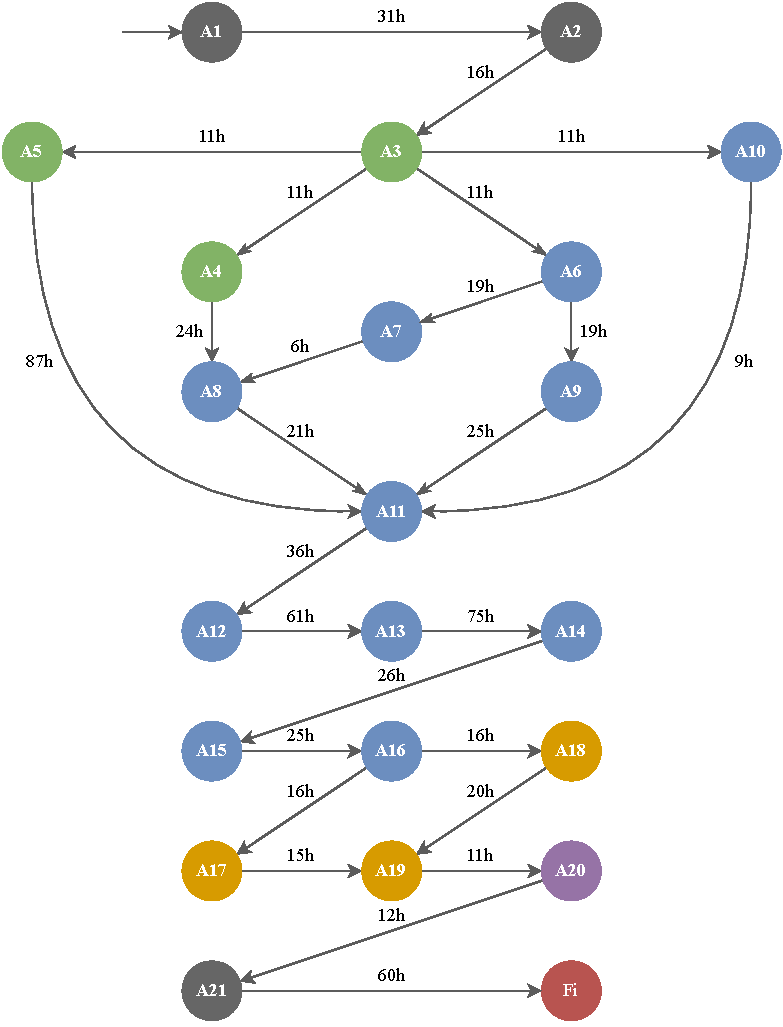
\includegraphics[width=0.9\textwidth]{assets/planification_figs/activityDiagram.pdf}
	\caption{\label{img:diagrama_activitats}Diagrama de les activitats planificades.}
\end{figure}

A partir del diagrama d'activitats, es pot saber fàcilment la durada màxima del projecte. Per calcular-la, cal sumar els temps de cadascuna de les activitats del camí crític del graf, és a dir, el camí des d'A1 fins a Fi més costós en temps.

\textbf{A1} $\rightarrow$ \textbf{A2} $\rightarrow$ \textbf{A5} $\rightarrow$ \textbf{A11} $\rightarrow$ \textbf{A12} $\rightarrow$ \textbf{A13} $\rightarrow$ \textbf{A14} $\rightarrow$ \textbf{A15} $\rightarrow$ \textbf{A16} $\rightarrow$ \textbf{A18} $\rightarrow$ \textbf{A19} $\rightarrow$ \textbf{A20} $\rightarrow$ \textbf{A21} $\rightarrow$ Fi

El resultat de la suma dels temps del camí crític i, per tant, la durada màxima estimada del projecte és de 427 hores. Si es suposen jornades de treball de 4 hores diàries i 5 dies a la setmana, el temps de desenvolupament del projecte seria de 21.35 setmanes (quasi bé 5 mesos).


\subsection{Cronograma}
\label{subsec:cronograma}

En aquesta subsecció, es representarà el diagrama de Gantt que recull la planificació del projecte.

\begin{figure}[H]
  \centering
  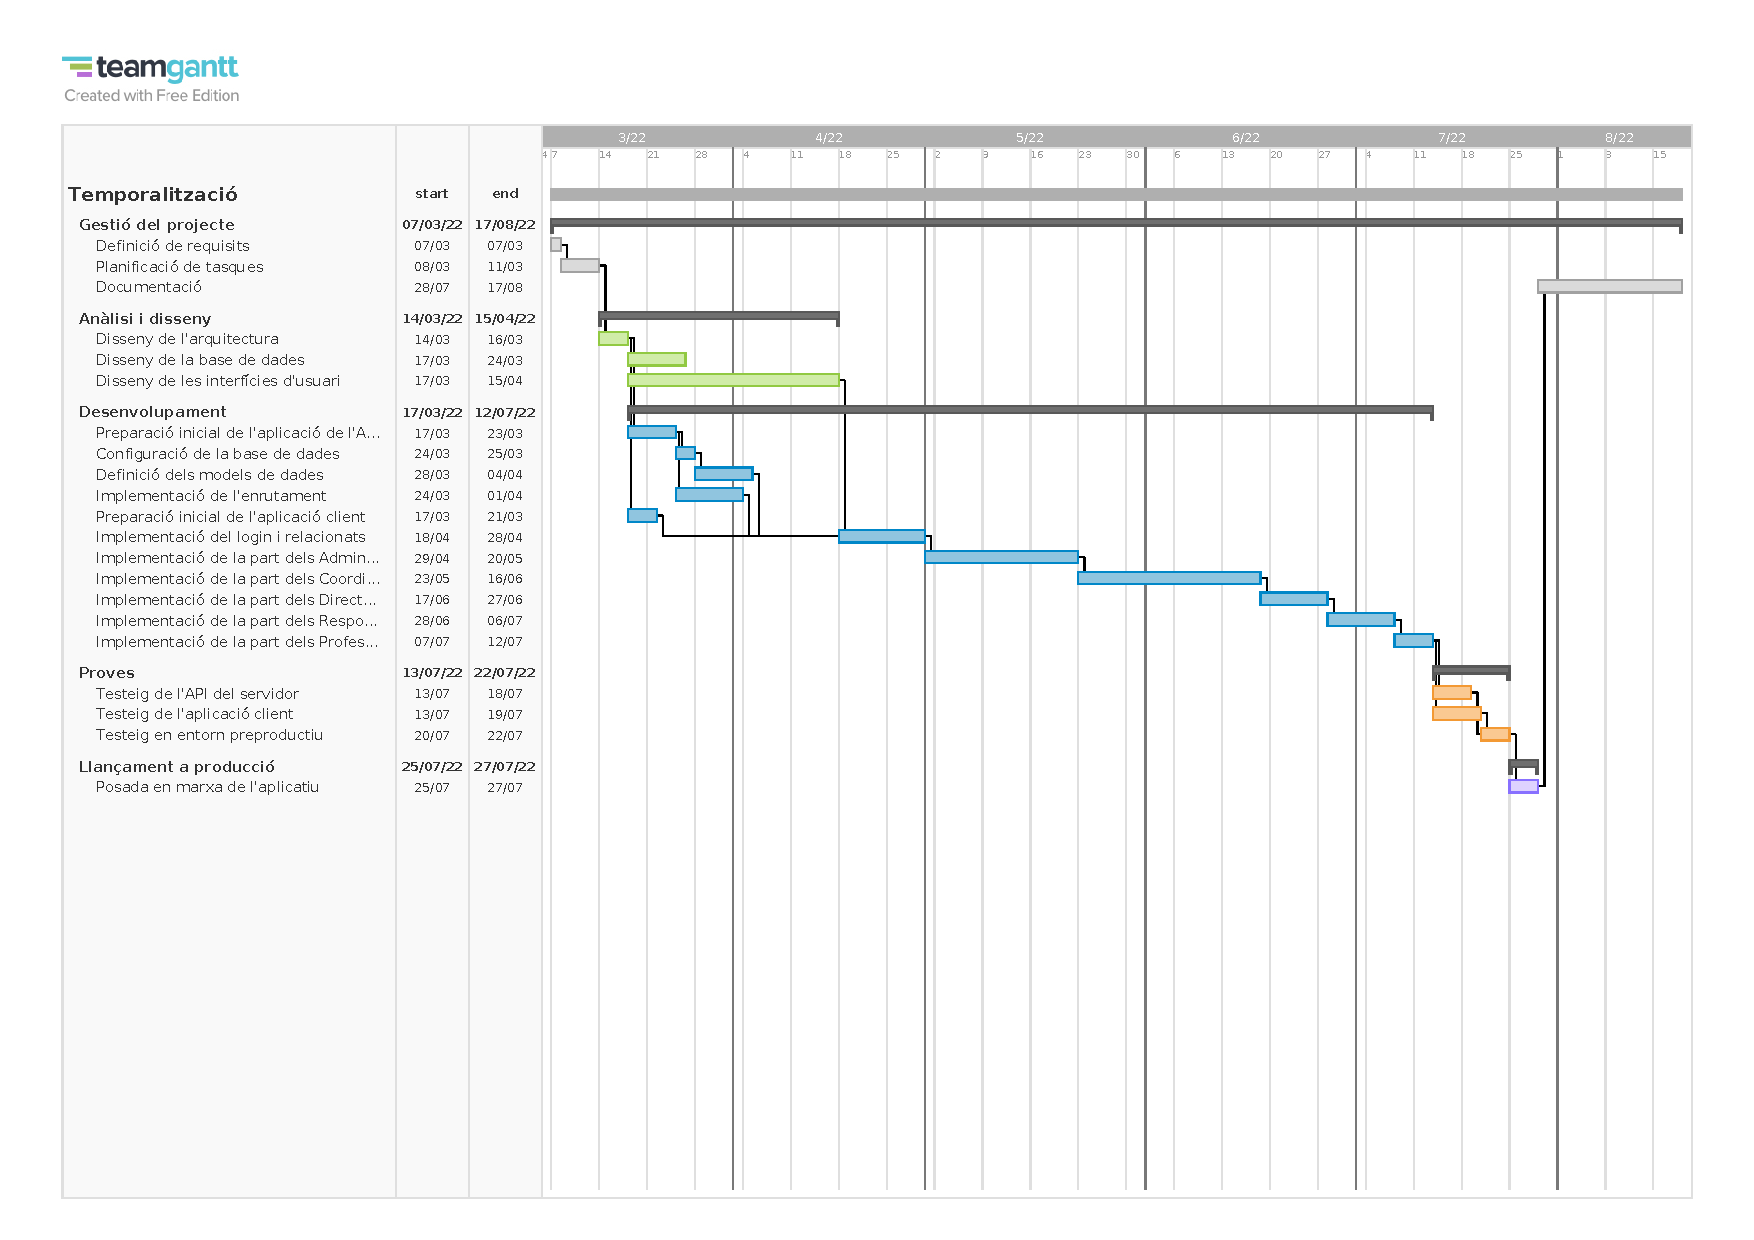
\includegraphics[width=1.3\textwidth, angle=90]{assets/planification_figs/ganttDiagram.pdf}
  \caption{\label{img:diagrama_gantt}Diagrama de Gantt.}
\end{figure}

Tal com es pot veure a la part esquerra del diagrama, a part de les activitats determinades a la subsecció~\ref{subsec:determinacio_activitats}, també hi apareixen les dates d'inici i de fi previstes per a cadascuna. Aquestes dates s'han calculat suposant jornades de treball de 4 hores diàries i 5 dies a la setmana.


\chapter{Estudis i decisions}
\label{cap:estudi}

\section{Gestió i estructura del projecte}
\label{sec:decisions_estructura}

\subsection{Control de versions}
\label{subsec:decisions_estructura_versions}

En aquesta subsecció, es justificarà l'el·lecció del sistema de control de versions utilitzat en el projecte: \textbf{Git}.

Disposar d'un sistema de control de versions a l'hora de desenvolupar una aplicació aporta un gran nombre d'avantatges, d'entre els quals destaca la capacitat de consultar o restaurar estats antics del codi i la de bifurcar el desenvolupament.

Git~\cite{Git} (veure figura~\ref{img:logo_git}), és el sistema de control de versions més popular amb diferència i, encara que existeixin algunes alternatives, és la que més funcionalitats ofereix i l'opció preferida de la gran majoria de desenvolupadors. A banda d'aquests motius, Git és l'única eina d'aquesta tipologia amb què tinc experiència. 

\begin{figure}[H]
  \centering
  
\includegraphics[width=0.2\textwidth]{assets/logos/Git.png}
  \caption{\label{img:logo_git}Logotip de Git.}
\end{figure}

Normalment, l'ús de Git sol acompanyar-se de l'allotjament dels repositoris a una plataforma web dedicada a aquesta funció. Aquests tipus de plataforma permeten evitar la pèrdua accidental del codi d'un projecte, a banda d'aportar incomptables funcionalitats per al treball col·laboratiu, entre d'altres.

Hi ha diverses alternatives pel que fa a aquest tipus de plataforma, com ara GitHub, GitLab o BitBucket. No obstant això, l'opció escollida per al projecte és \textbf{GitHub}~\cite{GitHub} (veure figura~\ref{img:logo_github}), ja que la domino més que la resta i em sento més còmode treballant-hi.

\begin{figure}[H]
  \centering
  
\includegraphics[width=0.26\textwidth]{assets/logos/GitHub.png}
  \caption{\label{img:logo_github}Logotip de GitHub.}
\end{figure}

\subsection{Estructura del projecte}
\label{subsec:decisions_estructura_estructura}

En aquesta subsecció, es justificarà l'el·lecció de l'estructura del sistema: \textbf{monorepositori}.

Tal com s'ha vist al capítol~\ref{cap:marcdetreball}, el projecte engloba el desenvolupament de dues apliacions: el client i el servidor. Aquestes aplicacions es poden estructurar de dues maneres diferents:
\begin{itemize}
  \item \texttt{Multirepositori:} Separar les dues aplicacions en respositoris diferents. 
  \item \texttt{Monorepositori:} Agrupar les dues aplicacions en el mateix repositori.
\end{itemize}

Els beneficis principals del multirepositori són que els repositoris individuals són més fàcils de gestionar i queden més nets i recollits. En canvi, encara que en el monorepositori passi el contrari, és un aspecte que no té gaire pes, ja que l'escala del projecte és petita. A més a més, aquesta alternativa ofereix avantatges més interessants, com ara una millor estandarització del codi i la possibilitat de la seva reutilització, entre d'altres.

A més a més, tal com es veurà a les seccions~\ref{sec:decisions_client} i~\ref{sec:decisions_servidor}, el llenguatge de programació amb què s'han desenvolupat les dues aplicacions és el mateix: JavaScript. Gràcies a això es pot utilitzar un mateix gestor de paquets per a les dues.

Els gestors de paquets de JavaScript actuals més populars també incorporen altres eines i utilitats que faciliten la gestió d'un monorepositori dividint-lo en diferents espais de treball. Permeten definir les dependències de cada espai de treball i també de comunes. Aquest fet fa que la instal·lació i actualització dels paquets sigui més ràpida i eficient que en el cas de l'estructuració del projecte en multirepositori. Per aquests motius i per comoditat, l'el·lecció per al projecte ha estat l'estructuració en monorepositori.

Pel que fa al gestor de paquets, s'ha optat per \textbf{npm}~\cite{npm} (veure figura~\ref{img:logo_npm}). Els motius d'aquesta el·lecció han estat, principalment, el coneixement previ de l'eina i que és el gestor de paquets estàndard de Node.js, l'entorn escollit per a l'aplicació servidor (veure secció~\ref{sec:decisions_servidor}).

\begin{figure}[H]
  \centering
  
\includegraphics[width=0.2\textwidth]{assets/logos/NPM.png}
  \caption{\label{img:logo_npm}Logotip de npm.}
\end{figure}

\section{Aplicació client}
\label{sec:decisions_client}

%\subsection{Introducció}
%\label{subsec:decisions_client_intro}



\subsection{\textit{Bundler}}
\label{subsec:decisions_client_bundler}



\begin{figure}[H]
  \centering
  
\includegraphics[width=0.16\textwidth]{assets/logos/Vite.png}
  \caption{\label{img:logo_vite}Logotip de Vite.}
\end{figure}

\subsection{\textit{Frameworks}}
\label{subsec:decisions_client_frameworks}
% Vue i quasar


\begin{figure}[H]
  \centering
  
\includegraphics[width=0.14\textwidth]{assets/logos/Vue.png}
  \caption{\label{img:logo_vue}Logotip de Vue.}
\end{figure}

\begin{figure}[H]
  \centering
  
\includegraphics[width=0.15\textwidth]{assets/logos/Quasar.png}
  \caption{\label{img:logo_quasar}Logotip de Quasar.}
\end{figure}

\subsection{Enrutament}
\label{subsec:decisions_client_enrutament}
% vue-router



\subsection{Gestió d'estats globals}
\label{subsec:decisions_client_estats}
% pinia


\begin{figure}[H]
  \centering
  
\includegraphics[width=0.12\textwidth]{assets/logos/Pinia.png}
  \caption{\label{img:logo_pinia}Logotip de Pinia.}
\end{figure}

\subsection{Proves}
\label{subsec:decisions_client_proves}
% Chrome dev tools amb vue extension.


\begin{figure}[H]
  \centering
  
\includegraphics[width=0.22\textwidth]{assets/logos/ChromeDevTools.png}
  \caption{\label{img:logo_chrome_dev_tools}Logotip de Chrome Dev Tools.}
\end{figure}

\section{Aplicació servidor}
\label{sec:decisions_servidor}

%\subsection{Introducció}
%\label{subsec:decisions_servidor_intro}



\subsection{Entorn i llenguatge de programació}
\label{subsec:decisions_servidor_entorn}
% node+nodemon

Node.js és un entorn d'execució de JavaScript multiplataforma i de codi obert que funciona fora del navegador i està orientat al processament d'events asíncrons. Està dissenyat principalment per crear aplicacions de xarxa escalables. L'escalabilitat és possible gràcies a la seva capacitat d'atendre múltiples connexions simultàniament sense cap possibilitat de bloqueig: utilitza un sol fil d'execució, el qual executa una funció (\textit{callback}) per a cada connexió. Si aquesta funció realitza una operació asíncrona, com ara comunicar-se amb un sistema gestor de bases de dades, Node.js no es bloqueja mentre espera que finalitzi l'operació, sinó que n'executa d'altres que tingui pendents, com per exemple atendre una altra connexió. No obstant això, un cop hagi acabat l'operació, continuarà amb l'execució de la funció.

\begin{figure}[H]
  \centering
  
\includegraphics[width=0.24\textwidth]{assets/logos/Node.png}
  \caption{\label{img:logo_node}Logotip de Node.js.}
\end{figure}

\subsection{\textit{Framework}}
\label{subsec:decisions_servidor_framework}

Express és el \textit{framework} que funciona sobre Node.js més popular. Destaca per ser molt lleuger, minimalista i flexible, a més de ser senzill d'utilitzar. Express proporciona al desenvolupador molts mètodes i utilitats que permeten la creació d'una API sòlida de manera relativament ràpida.

\begin{figure}[H]
  \centering
  
\includegraphics[width=0.24\textwidth]{assets/logos/Express.png}
  \caption{\label{img:logo_express}Logotip de Express.js.}
\end{figure}

\subsection{ORM}
\label{subsec:decisions_servidor_orm}
% Explicar els orms al capítol de marc de treball o aquí?



\begin{figure}[H]
  \centering
  
\includegraphics[width=0.25\textwidth]{assets/logos/Sequelize.png}
  \caption{\label{img:logo_sequelize}Logotip de Sequelize.}
\end{figure}

\subsection{Proves}
\label{subsec:decisions_servidor_proves}
% postman



\begin{figure}[H]
  \centering
  
\includegraphics[width=0.23\textwidth]{assets/logos/Postman.png}
  \caption{\label{img:logo_postman}Logotip de Postman.}
\end{figure}

\section{Base de dades}
\label{sec:decisions_bdd}

% \subsection{Introducció}
% \label{subsec:decisions_bdd_intro}



\subsection{Entorn d'execució}
\label{subsec:decisions_bdd_entorn}


\begin{figure}[H]
  \centering
  
\includegraphics[width=0.25\textwidth]{assets/logos/Docker.png}
  \caption{\label{img:logo_docker}Logotip de Docker.}
\end{figure}

\subsection{Sistema gestor de bases de dades}
\label{subsec:decisions_bdd_sgbd}



\begin{figure}[H]
  \centering
  
\includegraphics[width=0.2\textwidth]{assets/logos/MySQL.png}
  \caption{\label{img:logo_mysql}Logotip de MySQL.}
\end{figure}

\subsection{Proves}
\label{subsec:decisions_bdd_proves}



\begin{figure}[H]
  \centering
  
\includegraphics[width=0.13\textwidth]{assets/logos/DataGrip.png}
  \caption{\label{img:logo_datagrip}Logotip de DataGrip.}
\end{figure}

\section{Eines de desenvolupament}
\label{sec:decisions_desenvolupament}

% \subsection{Introducció}
% \label{subsec:decisions_desenvolupament_intro}



\subsection{Editor de codi}
\label{subsec:decisions_desenvolupament_editor}
% dir que a part de les eines indicades a les respectives seccions hi ha vs code
% vs code + ext



\begin{figure}[H]
  \centering
  
\includegraphics[width=0.15\textwidth]{assets/logos/VSCode.png}
  \caption{\label{img:logo_vscode}Logotip de Visual Studio Code.}
\end{figure}

\section{Confecció de la memòria}
\label{sec:decisions_memoria}

% \subsection{Introducció}
% \label{subsec:decisions_memoria_intro}



\subsection{Elaboració del document}
\label{subsec:decisions_memoria_document}
% latex



\begin{figure}[H]
  \centering
  
\includegraphics[width=0.27\textwidth]{assets/logos/LaTeX.png}
  \caption{\label{img:logo_latex}Logotip de LaTeX.}
\end{figure}

\subsection{Diagrames, esquemes i figures}
\label{subsec:decisions_memoria_figures}



\begin{figure}[H]
  \centering
  
\includegraphics[width=0.13\textwidth]{assets/logos/diagramsNet.png}
  \caption{\label{img:logo_diagrams}Logotip de Diagrams.net.}
\end{figure}

\subsection{Diagrama de Gantt}
\label{subsec:decisions_memoria_gantt}



\begin{figure}[H]
  \centering
  
\includegraphics[width=0.25\textwidth]{assets/logos/teamGantt.png}
  \caption{\label{img:logo_teamGantt}Logotip de Teamgantt.}
\end{figure}


\chapter{Anàlisi i disseny del sistema}
\label{cap:analisi}

\section{Anàlisi dels casos d'ús}
\label{sec:casos_us}

\subsection{Actors implicats}
\label{subsec:casos_us_actors}

En aquesta subsecció, es recolliran els actors que poden interactuar amb l'aplicació de manera externa. També s'indicaran les relacions d'especialització / generalització que estableixen.

\begin{figure}[H]
  \centering
  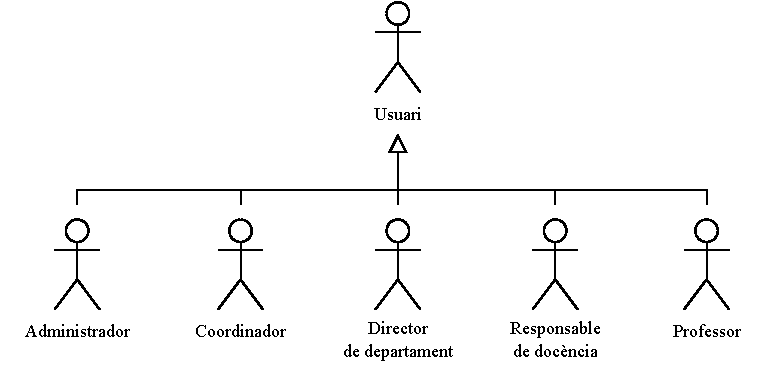
\includegraphics[width=\textwidth]{assets/use_cases/actors.pdf}
  \caption{\label{img:casos_us_actors}Jerarquia d'actors que poden interactuar amb l'aplicació.}
\end{figure}

Tal com es pot veure a la figura~\ref{img:casos_us_actors}, els actors es corresponen amb els diferents rols d'usuari que participen en l'aplicació. Tots aquests actors, que disposen del seu propi conjunt d'interaccions possibles amb el sistema, també hereten el d'\emph{Usuari}, ja que en són especialitzacions.

\subsection{Autenticació}
\label{subsec:casos_us_auth}

En aquesta subsecció, es representaran els casos d'ús relacionats amb la part de l'autenticació d'usuaris (veure figura~\ref{img:casos_us_auth}).

Quan es parli d'un \textit{Token}, s'estarà fent referència a un \textit{JSON Web Token}~\cite{JWT} generat per codificar certes dades amb una finalitat concreta (més informació al capítol~\ref{cap:implementacio}).

\begin{figure}[H]
  \centering
  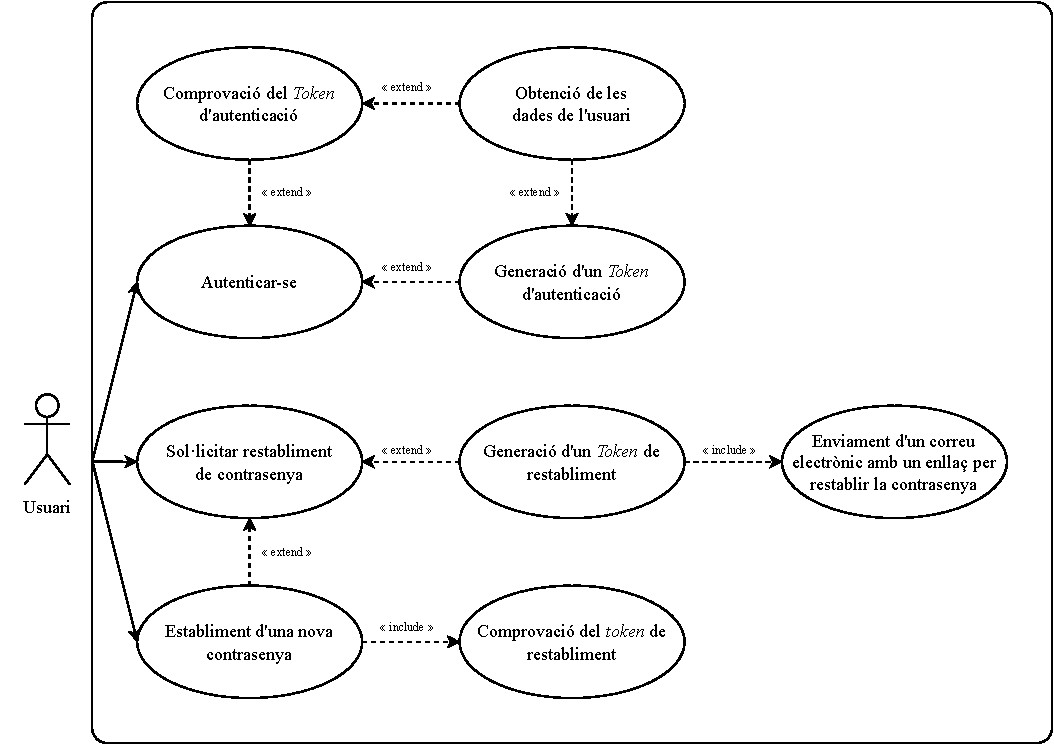
\includegraphics[width=\textwidth]{assets/use_cases/auth.pdf}
  \caption{\label{img:casos_us_auth}Diagrama dels casos d'ús relacionats amb l'autenticació.}
\end{figure}

\subsection{Gestió del pla docent}
\label{subsec:casos_us_pla}

\subsubsection{General}

En aquest apartat, es representaran els casos d'ús generals involucrats en la gestió del pla docent (veure figura~\ref{img:casos_us_pla_general}), els quals seran desglossats en els apartats posteriors de la subsecció.

\begin{figure}[H]
  \centering
  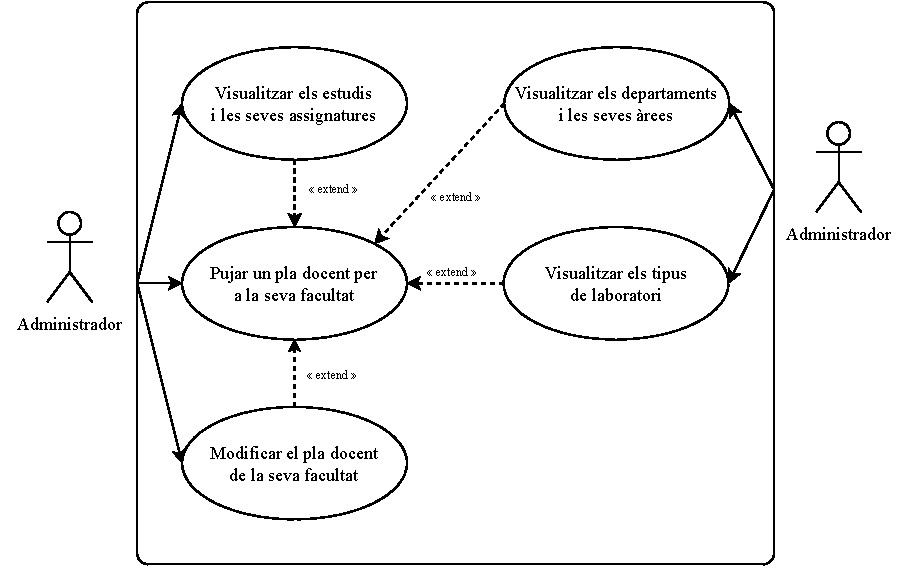
\includegraphics[width=0.9\textwidth]{assets/use_cases/pla_docent/general.pdf}
  \caption{\label{img:casos_us_pla_general}Diagrama de casos d'ús general de la gestió del pla docent.}
\end{figure}

\subsubsection{Pujada d'un pla docent}

En aquest apartat, es representaran els casos d'ús involucrats en la pujada d'un pla docent (veure figura~\ref{img:casos_us_pla_pujada}).

\begin{figure}[H]
  \centering
  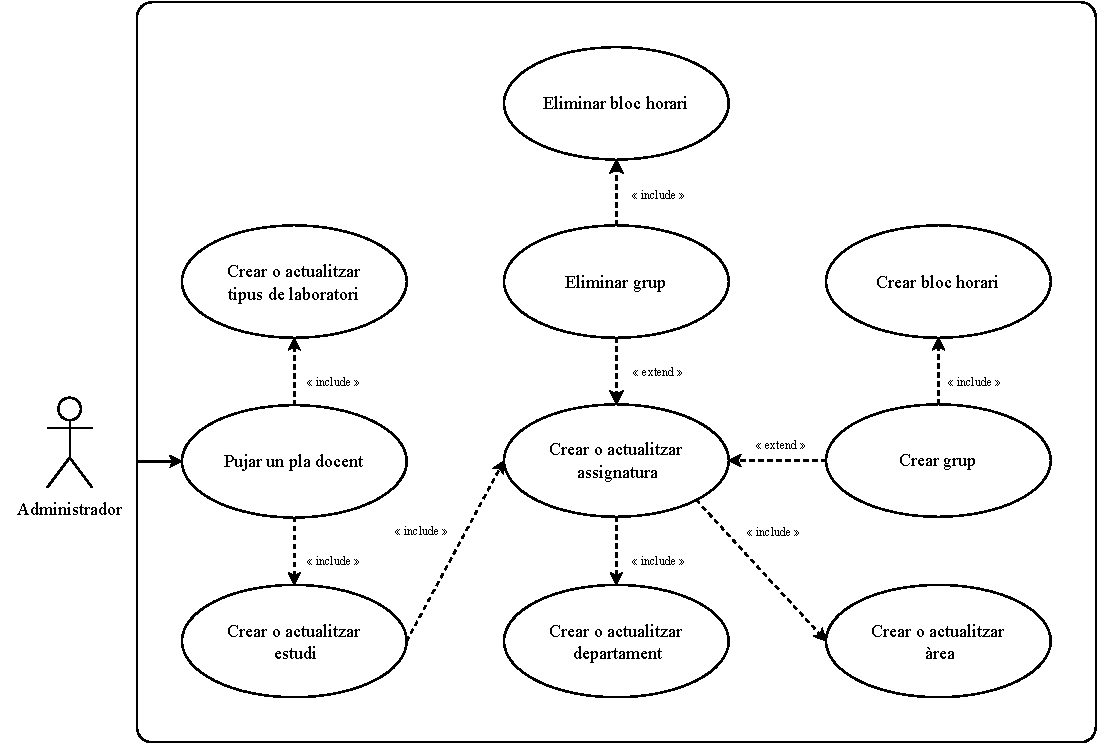
\includegraphics[width=\textwidth]{assets/use_cases/pla_docent/pujada.pdf}
  \caption{\label{img:casos_us_pla_pujada}Diagrama de casos d'ús de la pujada d'un pla docent.}
\end{figure}

\subsubsection{Modificació del pla docent}

En aquest apartat, es representaran els casos d'ús involucrats en la modificació d'un pla docent (veure figura~\ref{img:casos_us_pla_modif}).

\begin{figure}[H]
  \centering
  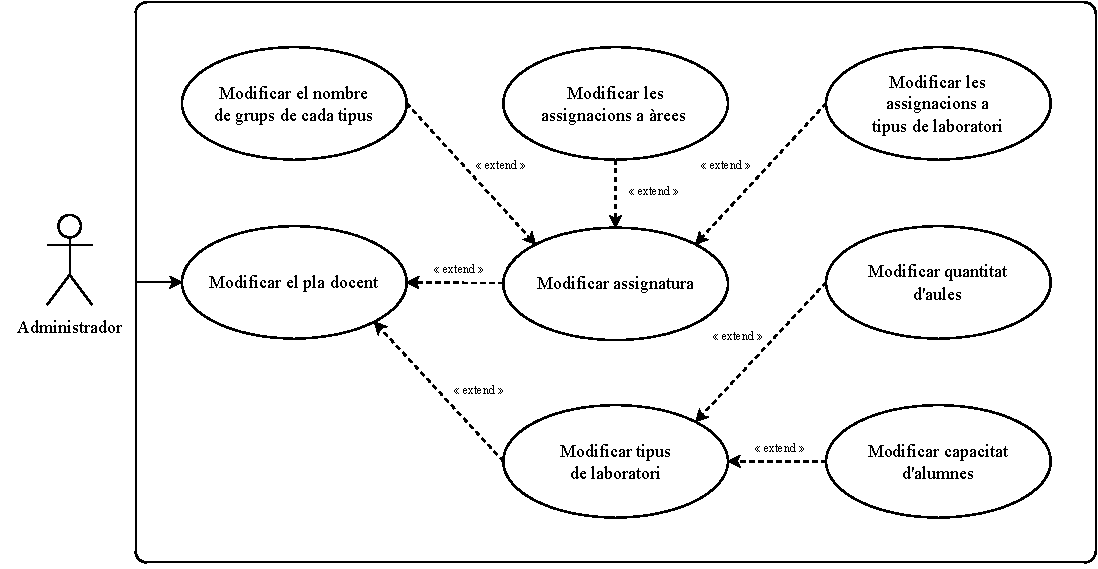
\includegraphics[width=\textwidth]{assets/use_cases/pla_docent/modif.pdf}
  \caption{\label{img:casos_us_pla_modif}Diagrama de casos d'ús de la modificació del pla docent.}
\end{figure}

\subsection{Gestió d'usuaris}
\label{subsec:casos_us_usuaris}

En aquesta subsecció, es representaran els casos d'ús involucrats en la gestió d'usuaris (veure figura~\ref{img:casos_us_usuaris}).

És important destacar que, per motius de llegibilitat, s'ha optat per representar només una vegada i de manera genèrica els casos d'ús ``Crear usuari'', ``Eliminar usuari'' i ``Reenviar correu d'activació''.

En realitat, aquests casos d'ús només s'apliquen a un usuari d'un rol concret, el qual és definit segons el rol dels usuaris que s'estiguin gestionant: en la gestió de Coordinadors, només s'apliquen a usuaris Coordinadors i així successivament.

\begin{figure}[H]
  \centering
  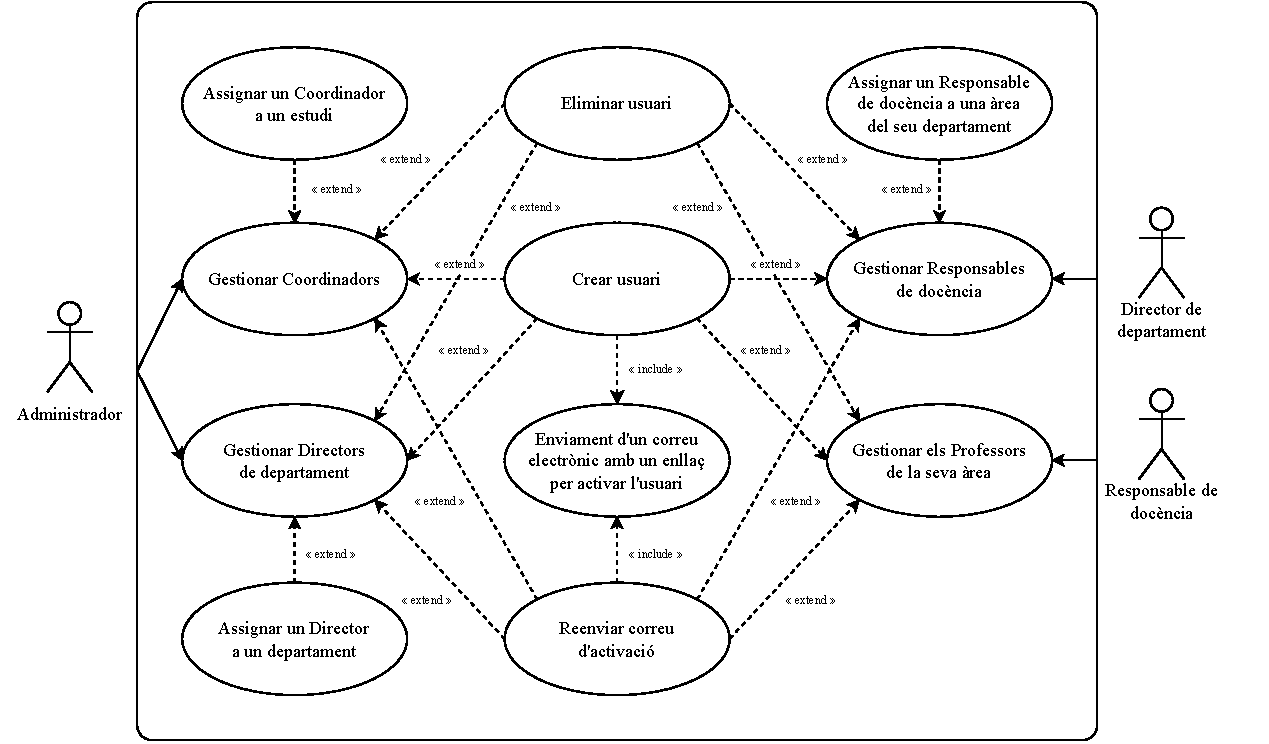
\includegraphics[width=\textwidth]{assets/use_cases/usuaris.pdf}
  \caption{\label{img:casos_us_usuaris}Diagrama de casos d'ús de la gestió d'usuaris.}
\end{figure}

\subsection{Visualització d'horaris}
\label{subsec:casos_us_veure_horaris}

En aquesta subsecció, es representaran els casos d'ús involucrats en la visualització d'horaris (veure figura~\ref{img:casos_us_veure_horaris}).

\begin{figure}[H]
  \centering
  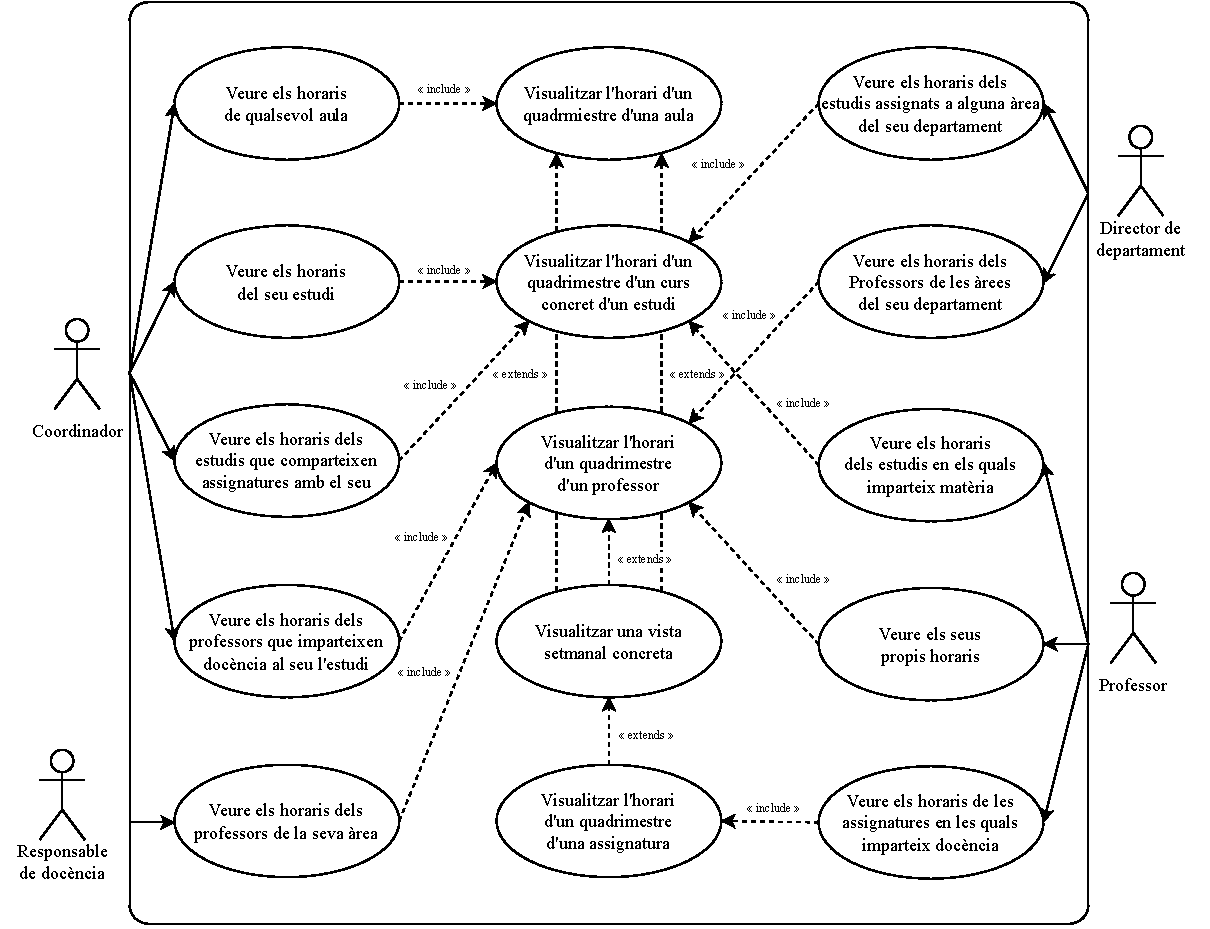
\includegraphics[width=\textwidth]{assets/use_cases/horaris/visualitzar.pdf}
  \caption{\label{img:casos_us_veure_horaris}Diagrama de casos d'ús de la visualització d'horaris.}
\end{figure}

\subsection{Modificació d'horaris d'estudis}
\label{subsec:casos_us_modif_horaris}

\subsubsection{General}

En aquest apartat, es representaran els casos d'ús generals involucrats en la modificació dels horaris dels estudis (veure figura~\ref{img:casos_us_modif_horaris_general}), els quals seran desglossats en els apartats posteriors de la subsecció.

\begin{figure}[H]
  \centering
  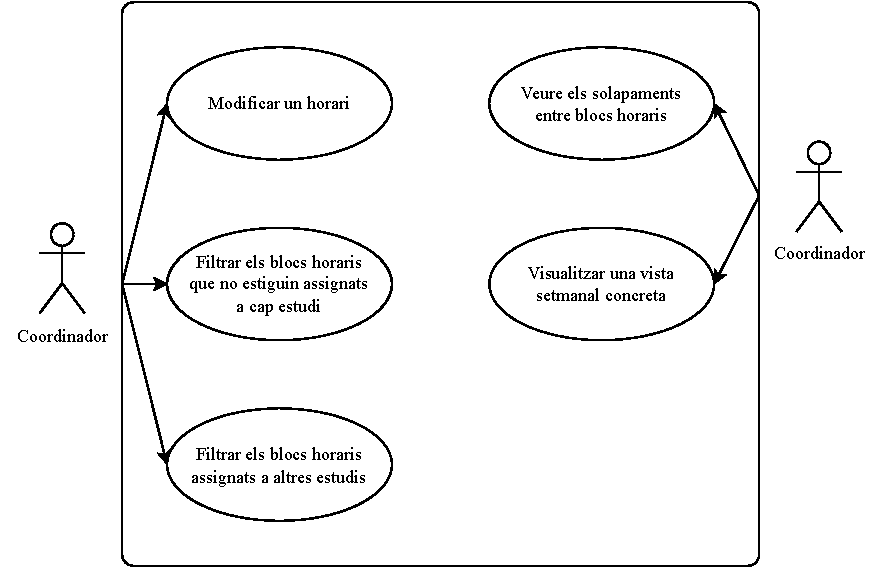
\includegraphics[width=0.9\textwidth]{assets/use_cases/horaris/modificar/general.pdf}
  \caption{\label{img:casos_us_modif_horaris_general}Diagrama de casos d'ús general de la modificació d'horaris.}
\end{figure}

\subsubsection{Modificació d'un horari d'un estudi}

En aquest apartat, es representaran els casos d'ús involucrats en la modificació d'un horari d'un estudi (veure figura~\ref{img:casos_us_horaris_modif}).

És important destacar que el cas d'ús ``Modificar un horari del seu estudi'' es refereix a la modificació de l'horari d'un quadrimestre d'un dels cursos de l'estudi que gestiona el Coordinador en qüestió.

A més a més, cal afegir que, per motius de llegibilitat, s'ha optat per representar només una vegada i de manera genèrica el cas d'ús ``Modificar dades relacionades amb el temps'', ja que serveix tant per blocs horaris com per blocs horaris genèrics.

\begin{figure}[H]
  \centering
  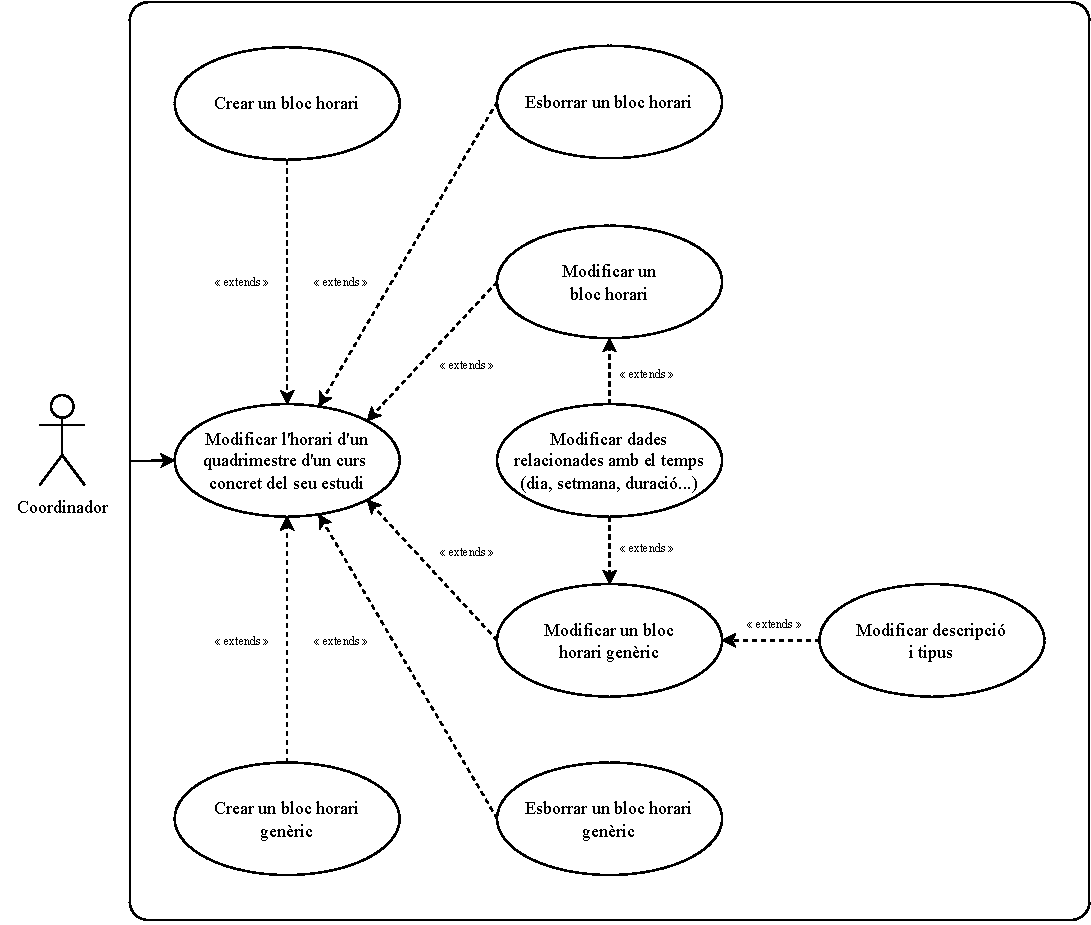
\includegraphics[width=\textwidth]{assets/use_cases/horaris/modificar/modif.pdf}
  \caption{\label{img:casos_us_horaris_modif}Diagrama de casos d'ús de la modificació d'un horari d'un estudi.}
\end{figure}

\subsubsection{Visualització de solapaments}

En aquest apartat, es representaran els casos d'ús involucrats en la visualització de solapaments entre blocs horaris (veure figura~\ref{img:casos_us_horaris_solap}).

És important destacar que el cas d'ús ``Veure els solapaments entre blocs horaris'' es refereix als solapaments existents a l'horari d'un quadrimestre d'un dels cursos de l'estudi que gestiona el Coordinador en qüestió.

\begin{figure}[H]
  \centering
  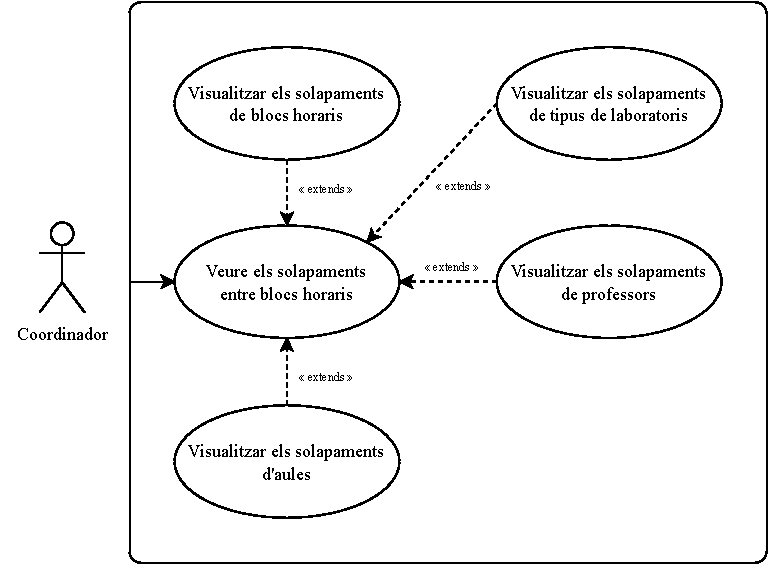
\includegraphics[width=0.9\textwidth]{assets/use_cases/horaris/modificar/solapaments.pdf}
  \caption{\label{img:casos_us_horaris_solap}Diagrama de casos d'ús de la visualització de solapaments.}
\end{figure}

\section{Disseny de la base de dades}
\label{sec:disseny_bdd}

\subsection{Model entitat-relació}
\label{subsec:bd_model_er}

En aquesta subsecció, es presentarà el diagrama entitat-relació dissenyat per emmagatzemar i gestionar adequadament les dades de l'aplicació (veure figura~\ref{img:db}).

Per tal d'evitar la rectificació manual del diagrama davant de qualsevol canvi en el disseny, s'ha optat per utilitzar una eina que en permeti la generació automàtica a partir de les taules que formin la base de dades. Més concretament, es tracta de DataGrip~\cite{DataGrip}.

La part negativa d'aquest programa és que no explicita la cardinalitat de les relacions. Per aquest motiu, és molt important remarcar que totes les relacions són ``u a molts'' exceptuant les següents que són ``u a u'':
\begin{itemize}
  \item \texttt{Estudi} (0..1) $\longrightarrow$ (0..1) \texttt{Usuari}.
  \item \texttt{Departament} (0..1) $\longrightarrow$ (0..1) \texttt{Usuari}.
  \item \texttt{Àrea} (0..1) $\longrightarrow$ (0..1) \texttt{Usuari}.
\end{itemize}

També cal tenir en compte que les relacions ``molts a molts'' hi apareixen ja ``aplicades'' amb la taula intermitja entre les dues entitats en qüestió, la qual és necessària per a la seva implementació. A més a més, l'herència d'usuaris també hi apareix ``resolta'' amb una implementació concreta (veure capítol~\ref{cap:estudi} per conèixer els detalls d'aquesta decisió).

\begin{figure}[H]
	\centering
	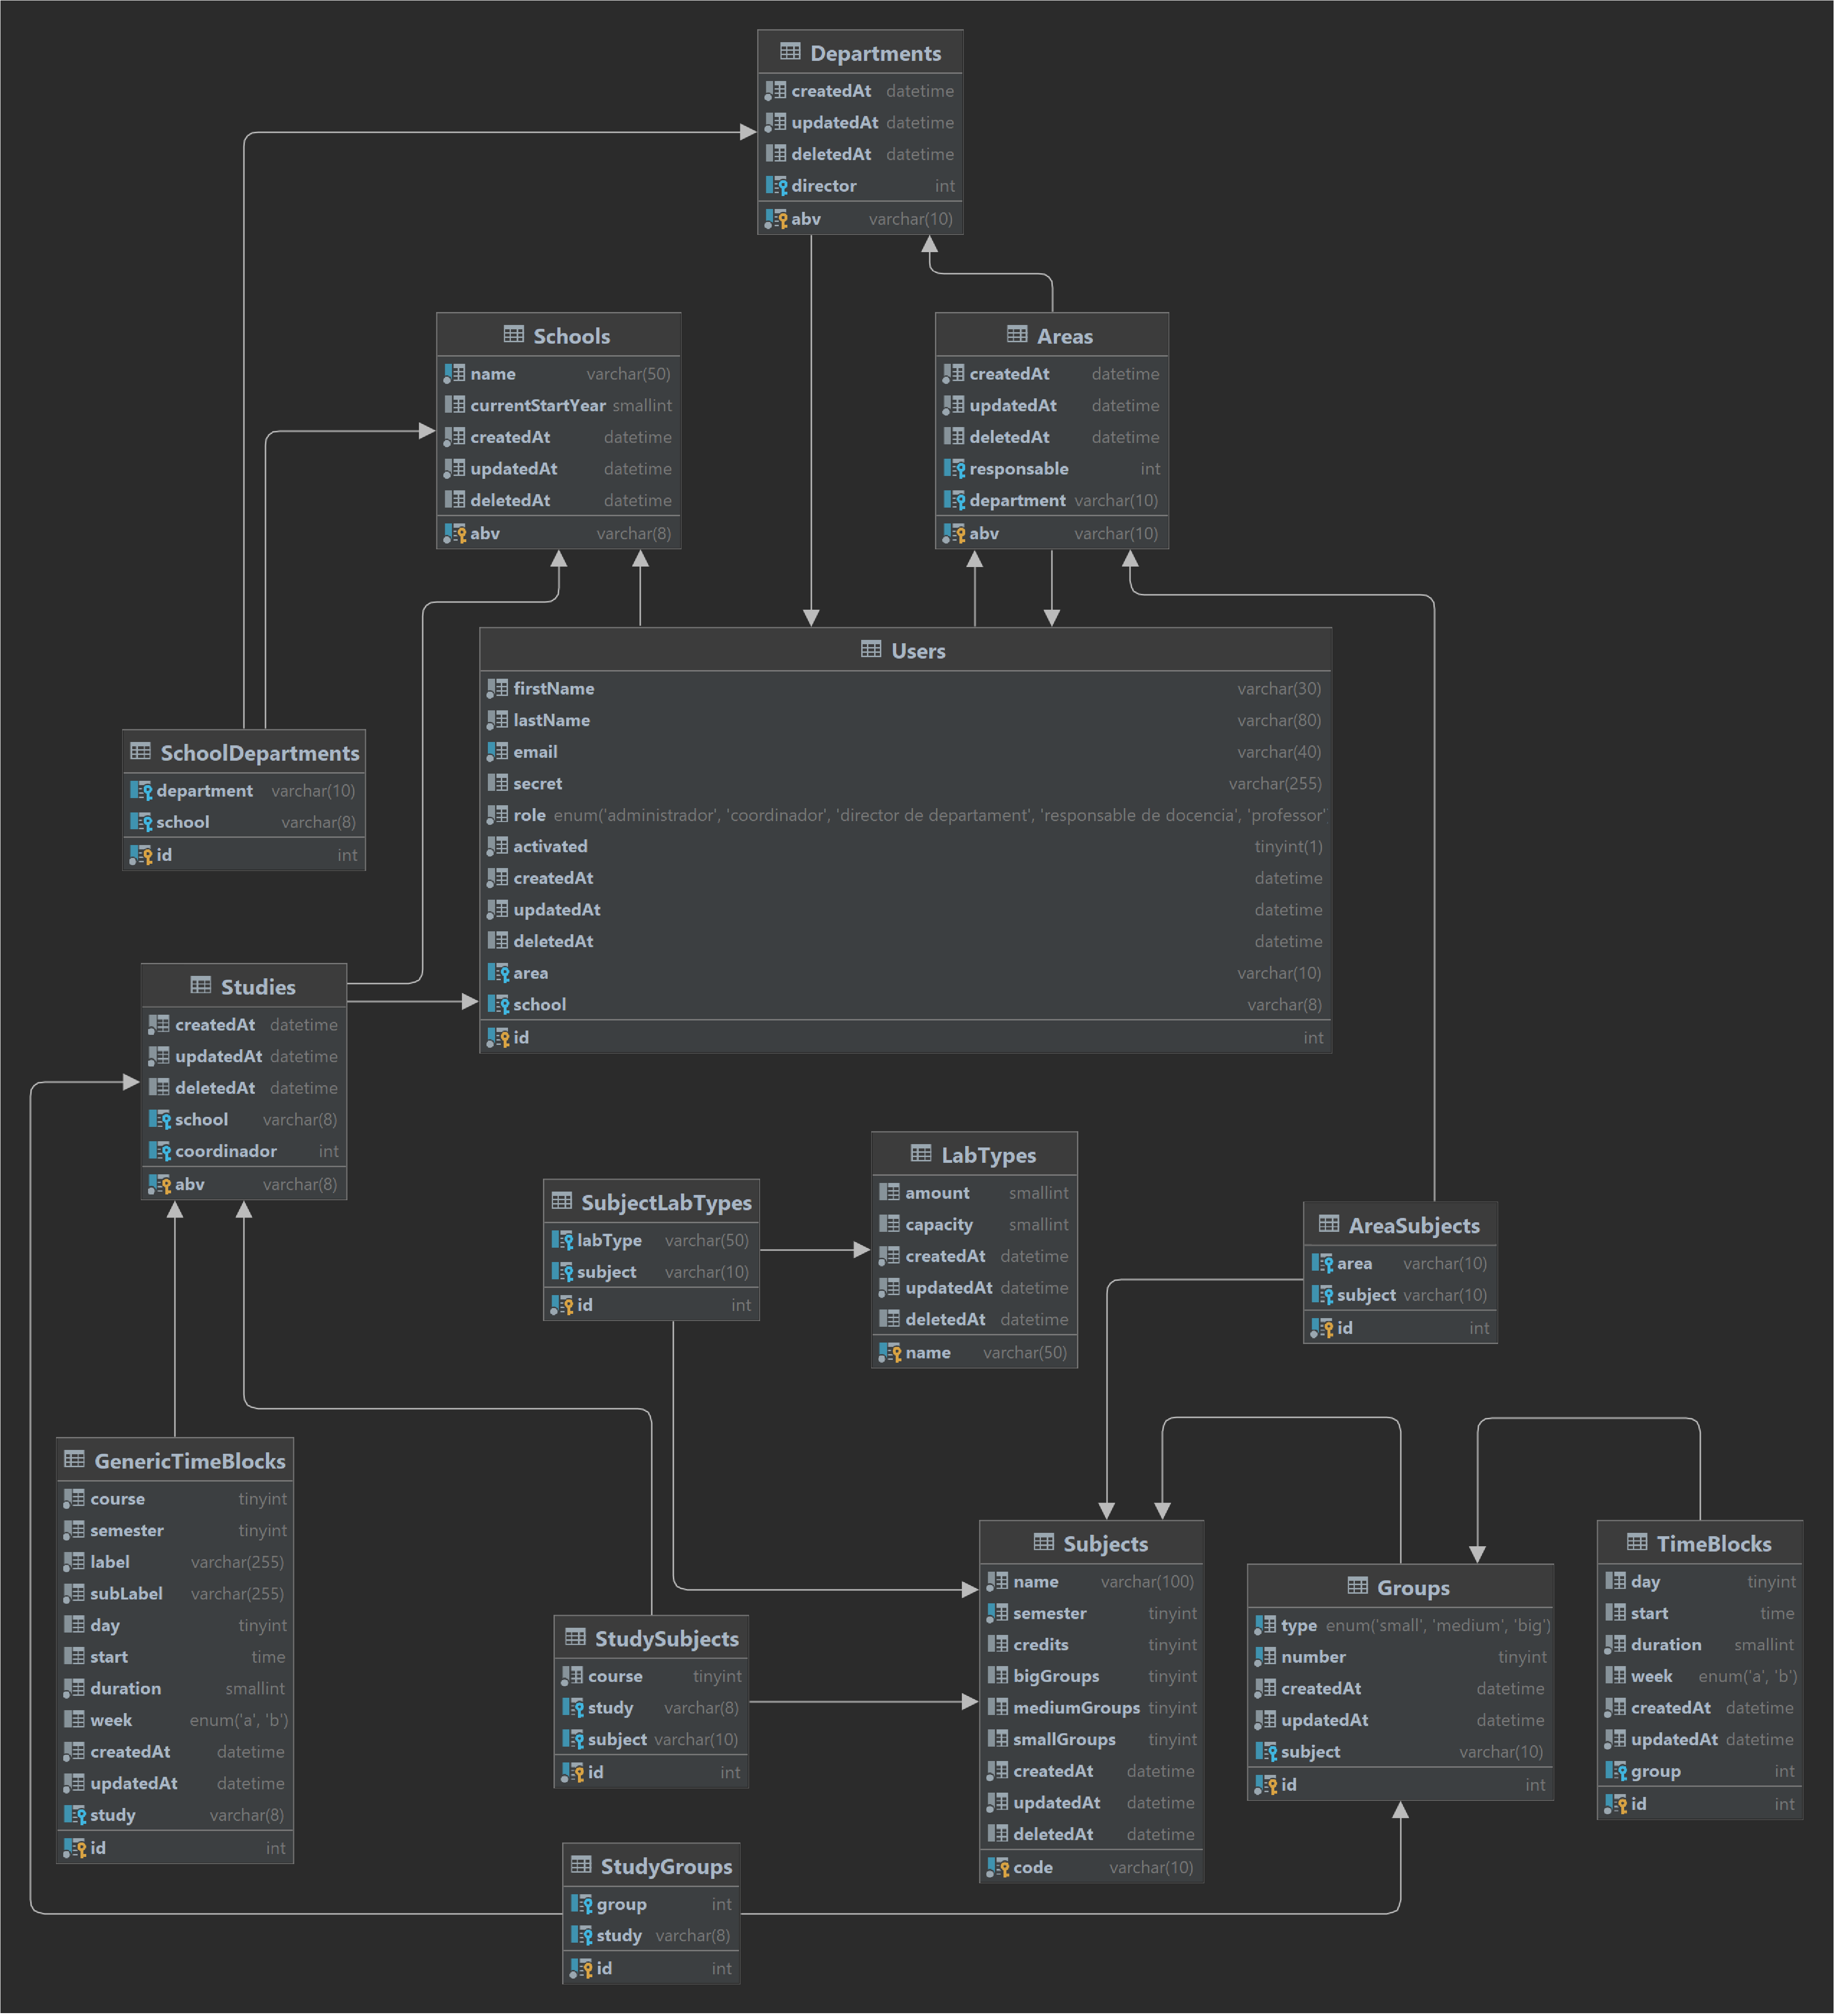
\includegraphics[width=\textwidth]{assets/db.pdf}
	\caption{\label{img:db}Diagrama relacional de la base de dades.}
\end{figure}

\subsection{Descripció de les entitats}
\label{subsec:bd_entitats}

\subsubsection{Consideracions inicials}

En aquest apartat, es presentaran una sèrie de consideracions inicials amb l'objectiu de clarificar el contingut dels que segueixen.

En primer lloc, és necessari definir el format que adoptarà cadascun dels atributs de les taules:
\\[8pt]
\centerline{\texttt{\textbf{Nom} <Tipus> [Restriccions]}: Descripció}

D'altra banda, cal destacar que totes les taules disposen de tres atributs comuns, els quals només es descriuen a continuació per tal d'evitar repeticions innecessàries:
\begin{itemize}
  \item \texttt{\textbf{createdAt} <datetime> [NOT NULL]}: Moment de la creació de l'entitat.
  \item \texttt{\textbf{updatedAt} <datetime> [NOT NULL]}: Moment de l'última modificació de l'entitat.
  \item \texttt{\textbf{deletedAt} <datetime>}: Moment de l'eliminació de l'entitat.
\end{itemize}

\subsubsection{Facultats o \textit{Schools}}

En aquest apartat, es descriuran els atributs de la taula ``Facultats'' (``\textit{Schools}'' al diagrama):
\begin{itemize}
  \item \texttt{\textbf{abv} <varchar(8)> [PRIMARY KEY]}: Abreviació (clau primària).
  \item \texttt{\textbf{name} <varchar(50)> [NOT NULL]}: Nom.
  \item \texttt{\textbf{currentStartYear} <smallint>}: Any d'inici del curs acadèmic actual.
\end{itemize}

\subsubsection{Usuaris o \textit{Users}}

En aquest apartat, es descriuran els atributs de la taula ``Usuaris'' (``\textit{Users}'' al diagrama):
\begin{itemize}
  \item \texttt{\textbf{id} <int> [PRIMARY KEY AUTOINCREMENT]}: Identificador numèric (clau primària).
  \item \texttt{\textbf{firstName} <varchar(30)> [NOT NULL]}: Nom.
  \item \texttt{\textbf{lastName} <varchar(80)> [NOT NULL]}: Cognoms.
  \item \texttt{\textbf{email} <varchar(40)> [NOT NULL]}: Adreça de correu electrònic.
  \item \texttt{\textbf{secret} <varchar(255)> [NOT NULL]}: Contrasenya (encriptada).
  \item \texttt{\textbf{role} <ENUM(<llista de rols>)> [NOT NULL]}: Rol.
  \item \texttt{\textbf{activated} <tinyint(1)> [DEFAULT 0]}: Indica si l'usuari ha estat activat o no.
  \item \texttt{\textbf{area} <varchar(10)>}: En cas que el rol sigui Professor, abreviació de l'àrea a la qual pertany (clau forana).
  \item \texttt{\textbf{school} <varchar(8)>}: Abreviació de la facultat a la qual pertany (clau forana).
\end{itemize}

\subsubsection{Departaments o \textit{Departments}}

En aquest apartat, es descriuran els atributs de la taula ``Departaments'' (``\textit{Departments}'' al diagrama):
\begin{itemize}
  \item \texttt{\textbf{abv} <varchar(10)> [PRIMARY KEY]}: Abreviació (clau primària).
  \item \texttt{\textbf{director} <int>}: Identificador numèric de l'usuari que el dirigeix (clau forana).
\end{itemize}

\subsubsection{FacultatDepartaments o \textit{SchoolDepartments}}

En aquest apartat, es descriuran els atributs de la taula ``FacultatDepartaments'' (``\textit{SchoolDepartments}'' al diagrama):
\begin{itemize}
  \item \texttt{\textbf{id} <int> [PRIMARY KEY]}: Identificador numèric (clau primària).
  \item \texttt{\textbf{school} <varchar(8)>}: Abreviació de la facultat a la qual pertany (clau forana).
  \item \texttt{\textbf{department} <varchar(10)>}: Abreviació del departament al qual pertany (clau forana).
\end{itemize}

Aquesta taula també conté un índex que assegura la unicitat de la parella d'atributs ``\textit{school}'' - ``\textit{department}''.

\subsubsection{Àrees o \textit{Areas}}

En aquest apartat, es descriuran els atributs de la taula ``Àrees'' (``\textit{Areas}'' al diagrama):
\begin{itemize}
  \item \texttt{\textbf{abv} <varchar(10)> [PRIMARY KEY]}: Abreviació (clau primària).
  \item \texttt{\textbf{responsable} <int>}: Identificador numèric de l'usuari que la gestiona (clau forana).
  \item \texttt{\textbf{departament} <int>}: Abreviació del departament al qual pertany (clau forana).
\end{itemize}

\subsubsection{Estudis o \textit{Studies}}

En aquest apartat, es descriuran els atributs de la taula ``Estudis'' (``\textit{Studies}'' al diagrama):
\begin{itemize}
  \item \texttt{\textbf{abv} <varchar(8)> [PRIMARY KEY]}: Abreviació (clau primària).
  \item \texttt{\textbf{school} <varchar(8)>}: Abreviació de la facultat a la qual pertany (clau forana).
  \item \texttt{\textbf{coordinador} <int>}: Identificador numèric de l'usuari que el gestiona (clau forana).
\end{itemize}

\subsubsection{Assignatures o \textit{Subjects}}

En aquest apartat, es descriuran els atributs de la taula ``Assignatures'' (``\textit{Subjects}'' al diagrama):
\begin{itemize}
  \item \texttt{\textbf{code} <varchar(10)> [PRIMARY KEY]}: Codi (clau primària).
  \item \texttt{\textbf{name} <varchar(100)> [NOT NULL]}: Nom.
  \item \texttt{\textbf{semester} <tinyint> [NOT NULL]}: Semestre durant el qual es cursa.
  \item \texttt{\textbf{credits} <tinyint>}: Nombre de crèdits.
  \item \texttt{\textbf{bigGroups} <tinyint>}: Nombre de grups grans que ha de tenir.
  \item \texttt{\textbf{mediumGroups} <tinyint>}: Nombre de grups mitjans que ha de tenir.
  \item \texttt{\textbf{smallGroups} <tinyint>}: Nombre de grups petits que ha de tenir.
\end{itemize}

\subsubsection{EstudiAssignatures o \textit{StudySubjects}}

En aquest apartat, es descriuran els atributs de la taula ``EstudiAssignatures'' (``\textit{StudySubjects}'' al diagrama):
\begin{itemize}
  \item \texttt{\textbf{id} <int> [PRIMARY KEY]}: Identificador numèric (clau primària).
  \item \texttt{\textbf{course} <tinyint> [NOT NULL]}: Curs en el qual es cursa l'assignatura a l'estudi.
  \item \texttt{\textbf{study} <varchar(8)>}: Abreviació de l'estudi al qual pertany (clau forana).
  \item \texttt{\textbf{subject} <varchar(10)>}: Codi de l'assignatura a la qual pertany (clau forana).
\end{itemize}

Aquesta taula també conté un índex que assegura la unicitat de la parella d'atributs ``\textit{study}'' - ``\textit{subject}''.

\subsubsection{ÀreaAssignatures o \textit{AreaSubjects}}

En aquest apartat, es descriuran els atributs de la taula ``ÀreaAssignatures'' (``\textit{AreaSubjects}'' al diagrama):
\begin{itemize}
  \item \texttt{\textbf{id} <int> [PRIMARY KEY]}: Identificador numèric (clau primària).
  \item \texttt{\textbf{area} <varchar(10)>}: Abreviació de l'àrea a la qual pertany (clau forana).
  \item \texttt{\textbf{subject} <varchar(10)>}: Codi de l'assignatura a la qual pertany (clau forana).
\end{itemize}

Aquesta taula també conté un índex que assegura la unicitat de la parella d'atributs ``\textit{area}'' - ``\textit{subject}''.

\subsubsection{TipusLaboratori o \textit{LabTypes}}

En aquest apartat, es descriuran els atributs de la taula ``TipusLaboratori'' (``\textit{LabTypes}'' al diagrama):
\begin{itemize}
  \item \texttt{\textbf{name} <varchar(50)> [PRIMARY KEY]}: Nom.
  \item \texttt{\textbf{amount} <smallint>}: Quantitat existent.
  \item \texttt{\textbf{capacity} <smallint>}: Capacitat d'alumnes.
\end{itemize}

\subsubsection{AssignaturaTipusLaboratori o \textit{SubjectLabTypes}}

En aquest apartat, es descriuran els atributs de la taula ``AssignaturaTipusLaboratori'' (``\textit{SubjectLabTypes}'' al diagrama):
\begin{itemize}
  \item \texttt{\textbf{id} <int> [PRIMARY KEY]}: Identificador numèric (clau primària).
  \item \texttt{\textbf{labType} <varchar(50)>}: Nom del tipus de laboratori al qual pertany (clau forana).
  \item \texttt{\textbf{subject} <varchar(10)>}: Codi de l'assignatura a la qual pertany (clau forana).
\end{itemize}

Aquesta taula també conté un índex que assegura la unicitat de la parella d'atributs ``\textit{labType}'' - ``\textit{subject}''.

\subsubsection{Grups o \textit{Groups}}

En aquest apartat, es descriuran els atributs de la taula ``Grups'' (``\textit{Groups}'' al diagrama):
\begin{itemize}
  \item \texttt{\textbf{id} <int> [PRIMARY KEY]}: Identificador numèric (clau primària).
  \item \texttt{\textbf{type} <enum(`small', `medium', `big')> [NOT NULL]}: Tipus.
  \item \texttt{\textbf{number} <tinyint> [NOT NULL]}: Número (numeració segons tipus).
  \item \texttt{\textbf{subject} <varchar(10)>}: Codi de l'assignatura a la qual pertany (clau forana).
\end{itemize}

\subsubsection{EstudiGrups o \textit{StudyGroups}}

En aquest apartat, es descriuran els atributs de la taula ``EstudiGrups'' (``\textit{StudyGroups}'' al diagrama):
\begin{itemize}
  \item \texttt{\textbf{id} <int> [PRIMARY KEY]}: Identificador numèric (clau primària).
  \item \texttt{\textbf{group} <int>}: Identificador numèric del grup al qual pertany (clau forana).
  \item \texttt{\textbf{study} <varchar(8)>}: Abreviació de l'estudi al qual pertany (clau forana).
\end{itemize}

Aquesta taula també conté un índex que assegura la unicitat de la parella d'atributs ``\textit{group}'' - ``\textit{study}''.

\subsubsection{BlocsHoraris o \textit{TimeBlocks}}

En aquest apartat, es descriuran els atributs de la taula ``BlocsHoraris'' (``\textit{TimeBlocks}'' al diagrama):
\begin{itemize}
  \item \texttt{\textbf{id} <int> [PRIMARY KEY]}: Identificador numèric (clau primària).
  \item \texttt{\textbf{day} <tinyint>}: Dia de la setmana al qual està assignat.
  \item \texttt{\textbf{start} <time>}: Hora d'inici.
  \item \texttt{\textbf{duration} <smallint> [NOT NULL]}: Duració.
  \item \texttt{\textbf{week} <enum(`A', `B')>}: Setmana a la qual està assignat (NULL si ho està a totes).
  \item \texttt{\textbf{group} <int>}: Identificador numèric del grup al qual pertany (clau forana).
\end{itemize}

\subsubsection{BlocsHorarisGenèrics o \textit{GenericTimeBlocks}}

En aquest apartat, es descriuran els atributs de la taula ``BlocsHorarisGenèrics'' (``\textit{GenericTimeBlocks}'' al diagrama):
\begin{itemize}
  \item \texttt{\textbf{id} <int> [PRIMARY KEY]}: Identificador numèric (clau primària).
  \item \texttt{\textbf{course} <tinyint> [NOT NULL]}: Curs al qual pertany.
  \item \texttt{\textbf{semester} <tinyint> [NOT NULL]}: Semestre al qual pertany.
  \item \texttt{\textbf{label} <varchar(255)> [NOT NULL]}: Etiqueta.
  \item \texttt{\textbf{subLabel} <varchar(255)> [NOT NULL]}: Subetiqueta.
  \item \texttt{\textbf{day} <tinyint>}: Dia de la setmana al qual està assignat.
  \item \texttt{\textbf{start} <time>}: Hora d'inici.
  \item \texttt{\textbf{duration} <smallint> [NOT NULL]}: Duració.
  \item \texttt{\textbf{week} <enum(`A', `B')>}: Setmana a la qual està assignat (NULL si ho està a totes).
  \item \texttt{\textbf{study} <varchar(8)>}: Abreviació de l'estudi al qual està assignat (clau forana).
\end{itemize}

\section{Interfícies d'usuari}
\label{sec:interficies_usuari}

En aquesta secció, s'exposarà el disseny de les diferents finestres que conformaran l'aplicació web client.

Cal destacar que l'aparença final de l'aplicació no ha de ser necessàriament igual que la que es mostrarà a les subseccions següents.

\subsection{Interfícies d'autenticació}
\label{subsec:interficies_auth}

En aquesta subsecció, es presentarà el disseny de les finestres més importants relacionades amb la part de l'autenticació.

A la figura~\ref{img:login} es pot veure el disseny de la finestra en la qual un usuari pot autenticar-se o bé indicar que ha oblidat la seva contrasenya.
\begin{figure}[H]
	\centering
	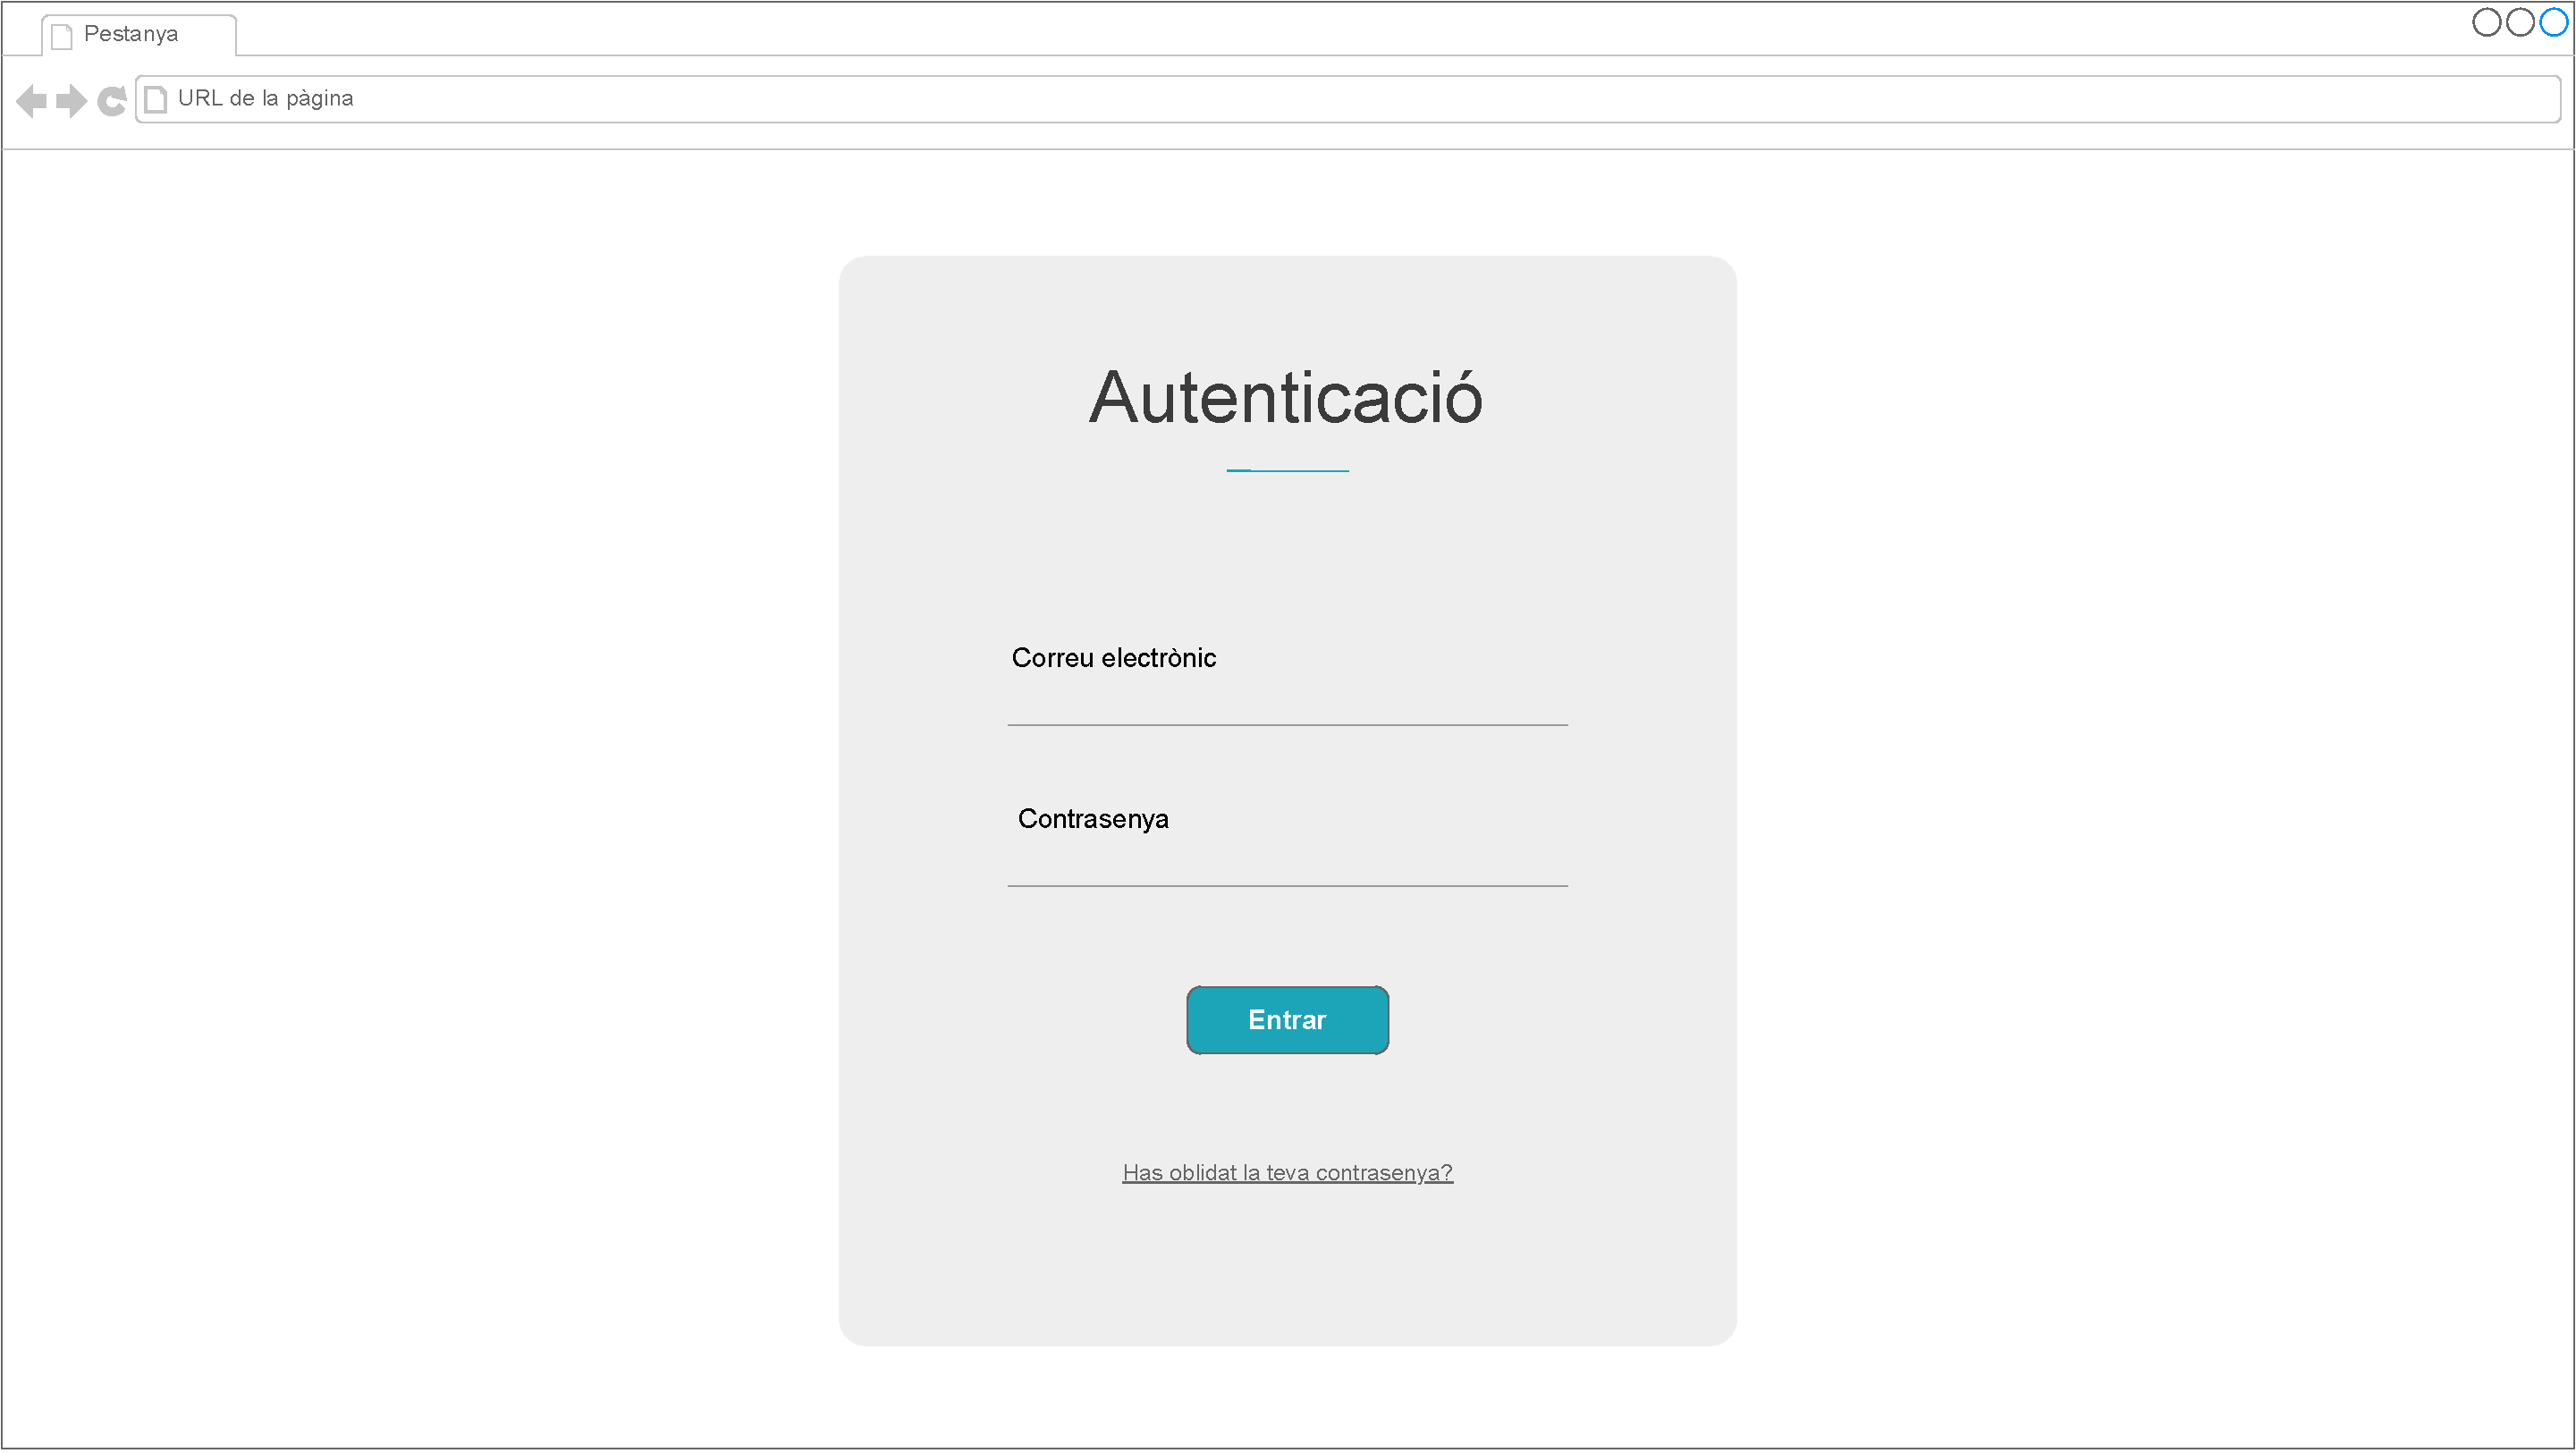
\includegraphics[width=\textwidth]{assets/interfaces/auth/login.pdf}
	\caption{\label{img:login}Disseny de la interfície d'autenticació.}
\end{figure}

A la figura~\ref{img:passwordRestablishment} es pot veure el disseny de la finestra en la qual un usuari pot introduir la seva adreça de correu electrònic per tal de restablir la seva contrasenya o bé tornar a la finestra d'autenticació.
\begin{figure}[H]
	\centering
	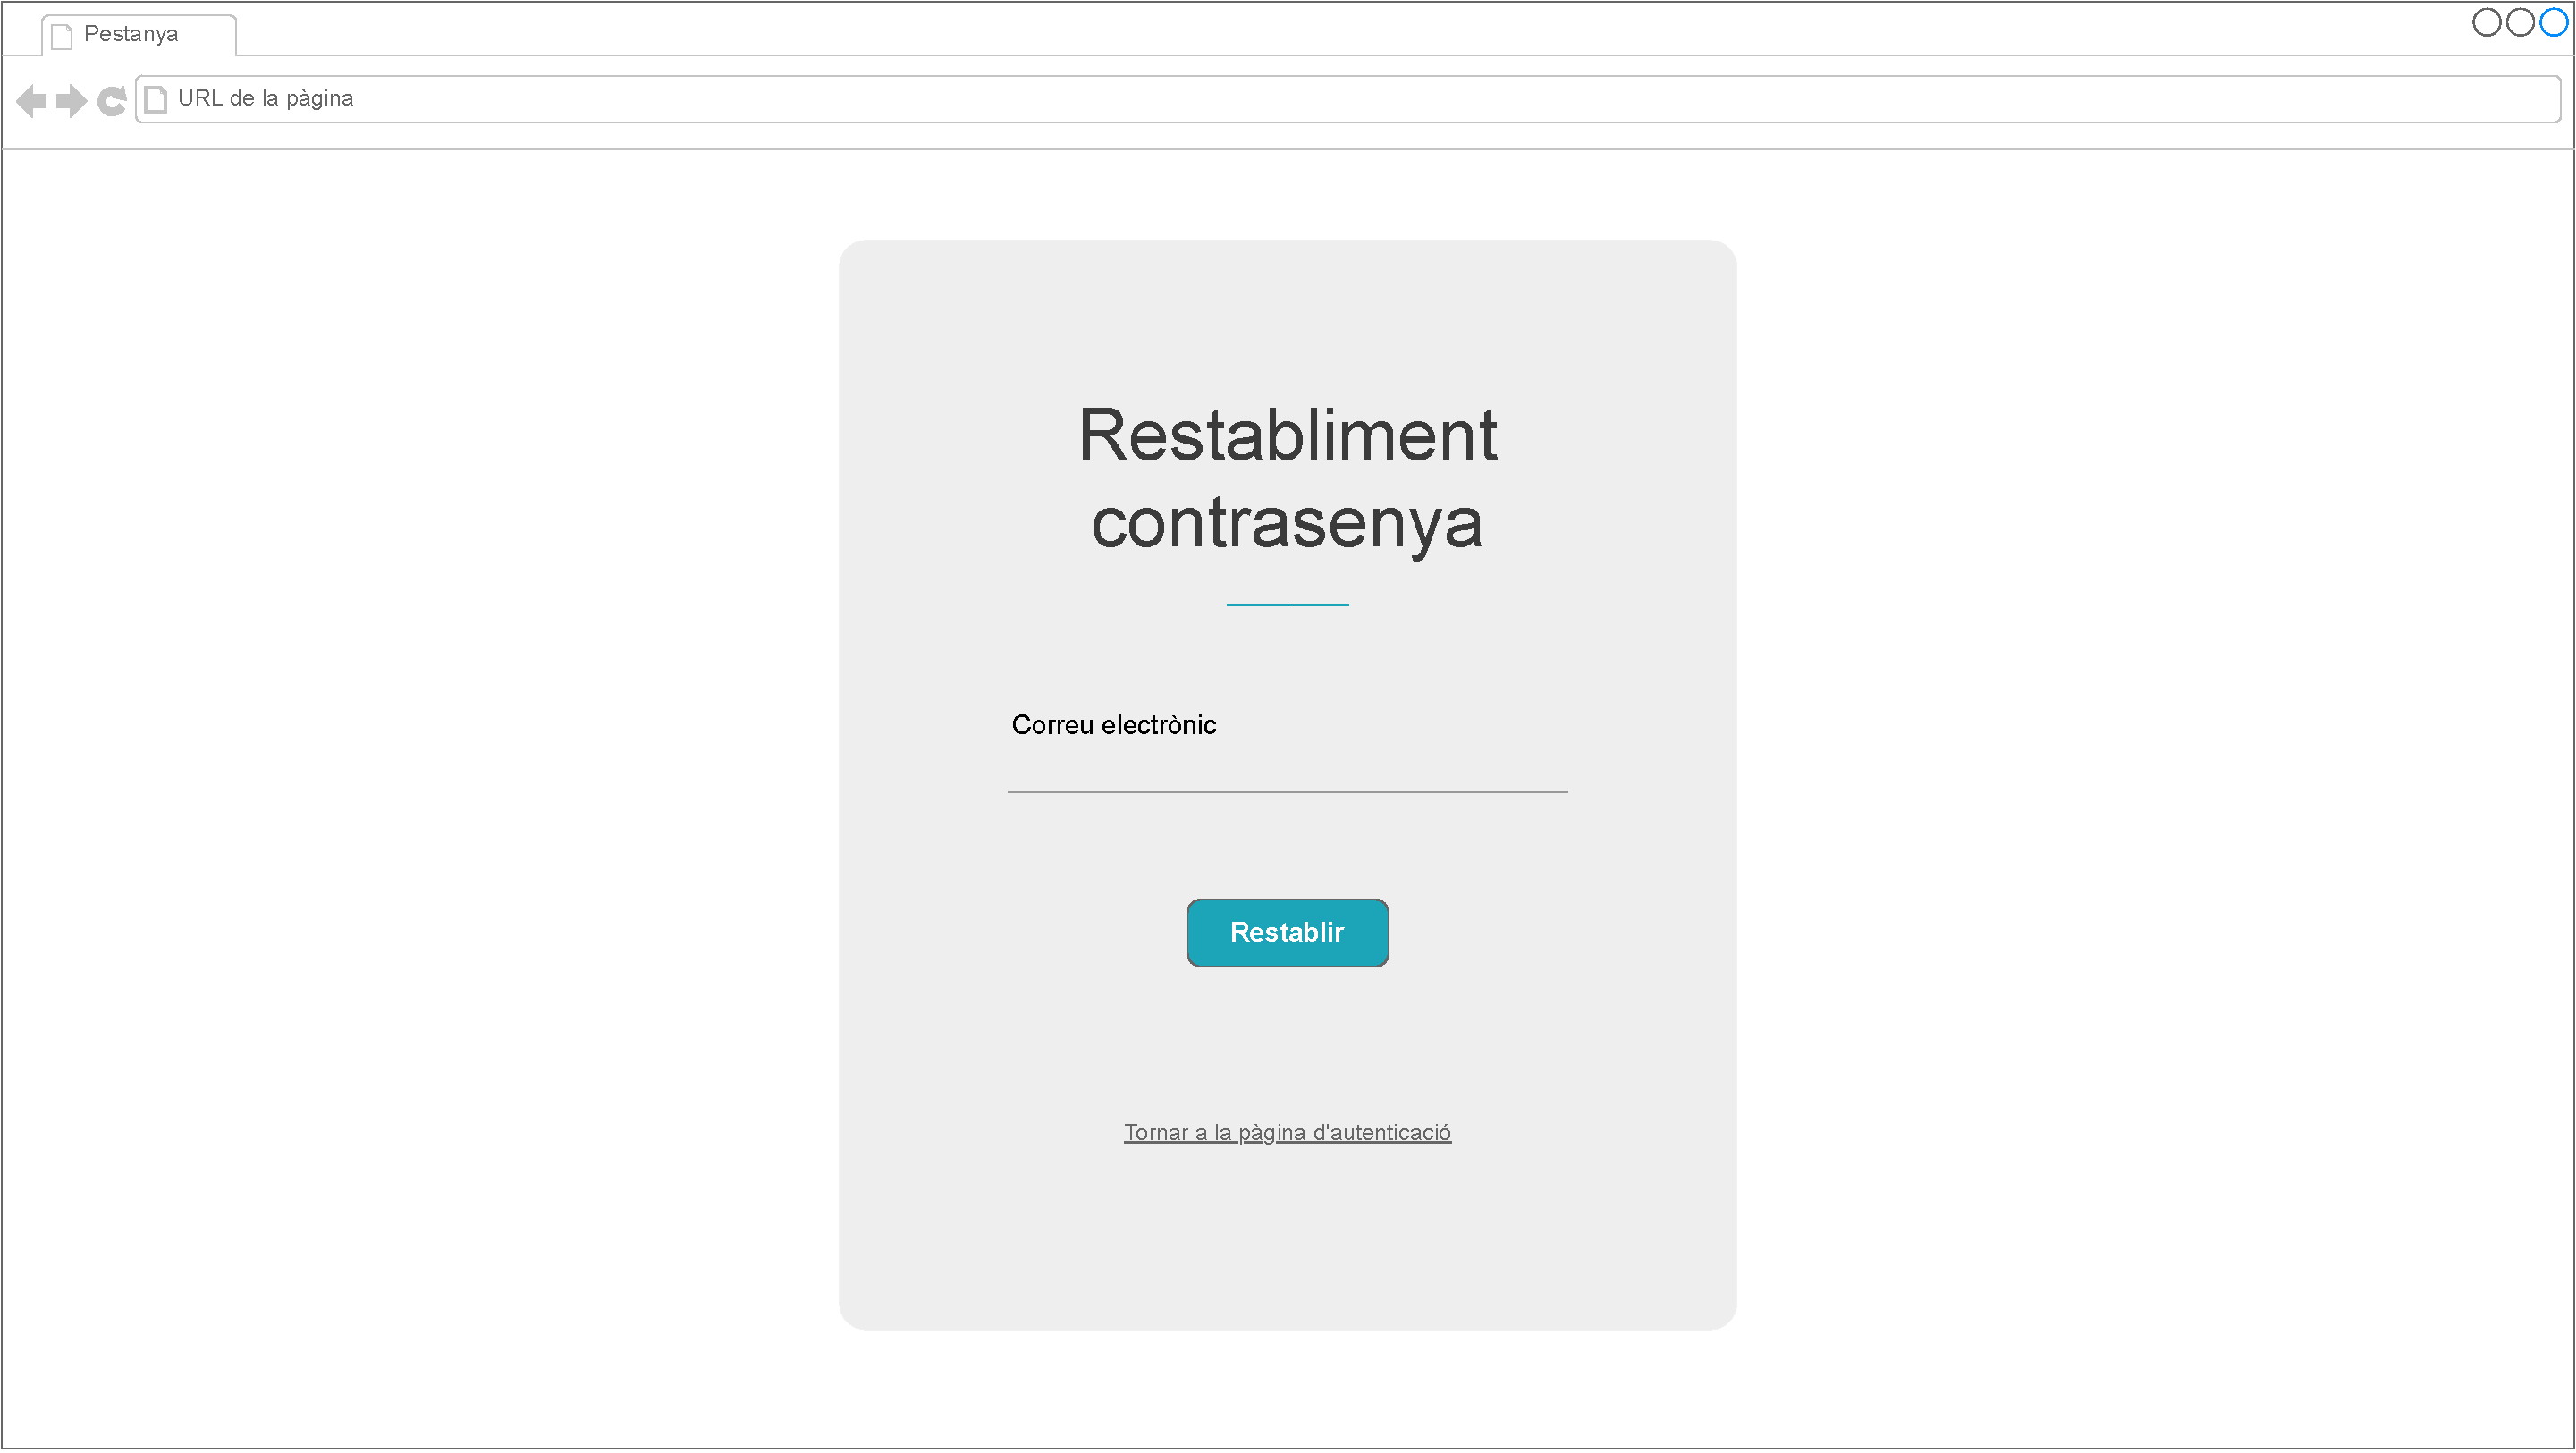
\includegraphics[width=\textwidth]{assets/interfaces/auth/passwordRestablishment.pdf}
	\caption{\label{img:passwordRestablishment}Disseny de la interfície de restabliment de contrasenya.}
\end{figure}

A la figura~\ref{img:passwordRestablished} es pot veure el disseny de la finestra en la qual s'informa l'usuari que se li ha enviat un correu electrònic per restablir la seva contrasenya.
\begin{figure}[H]
	\centering
	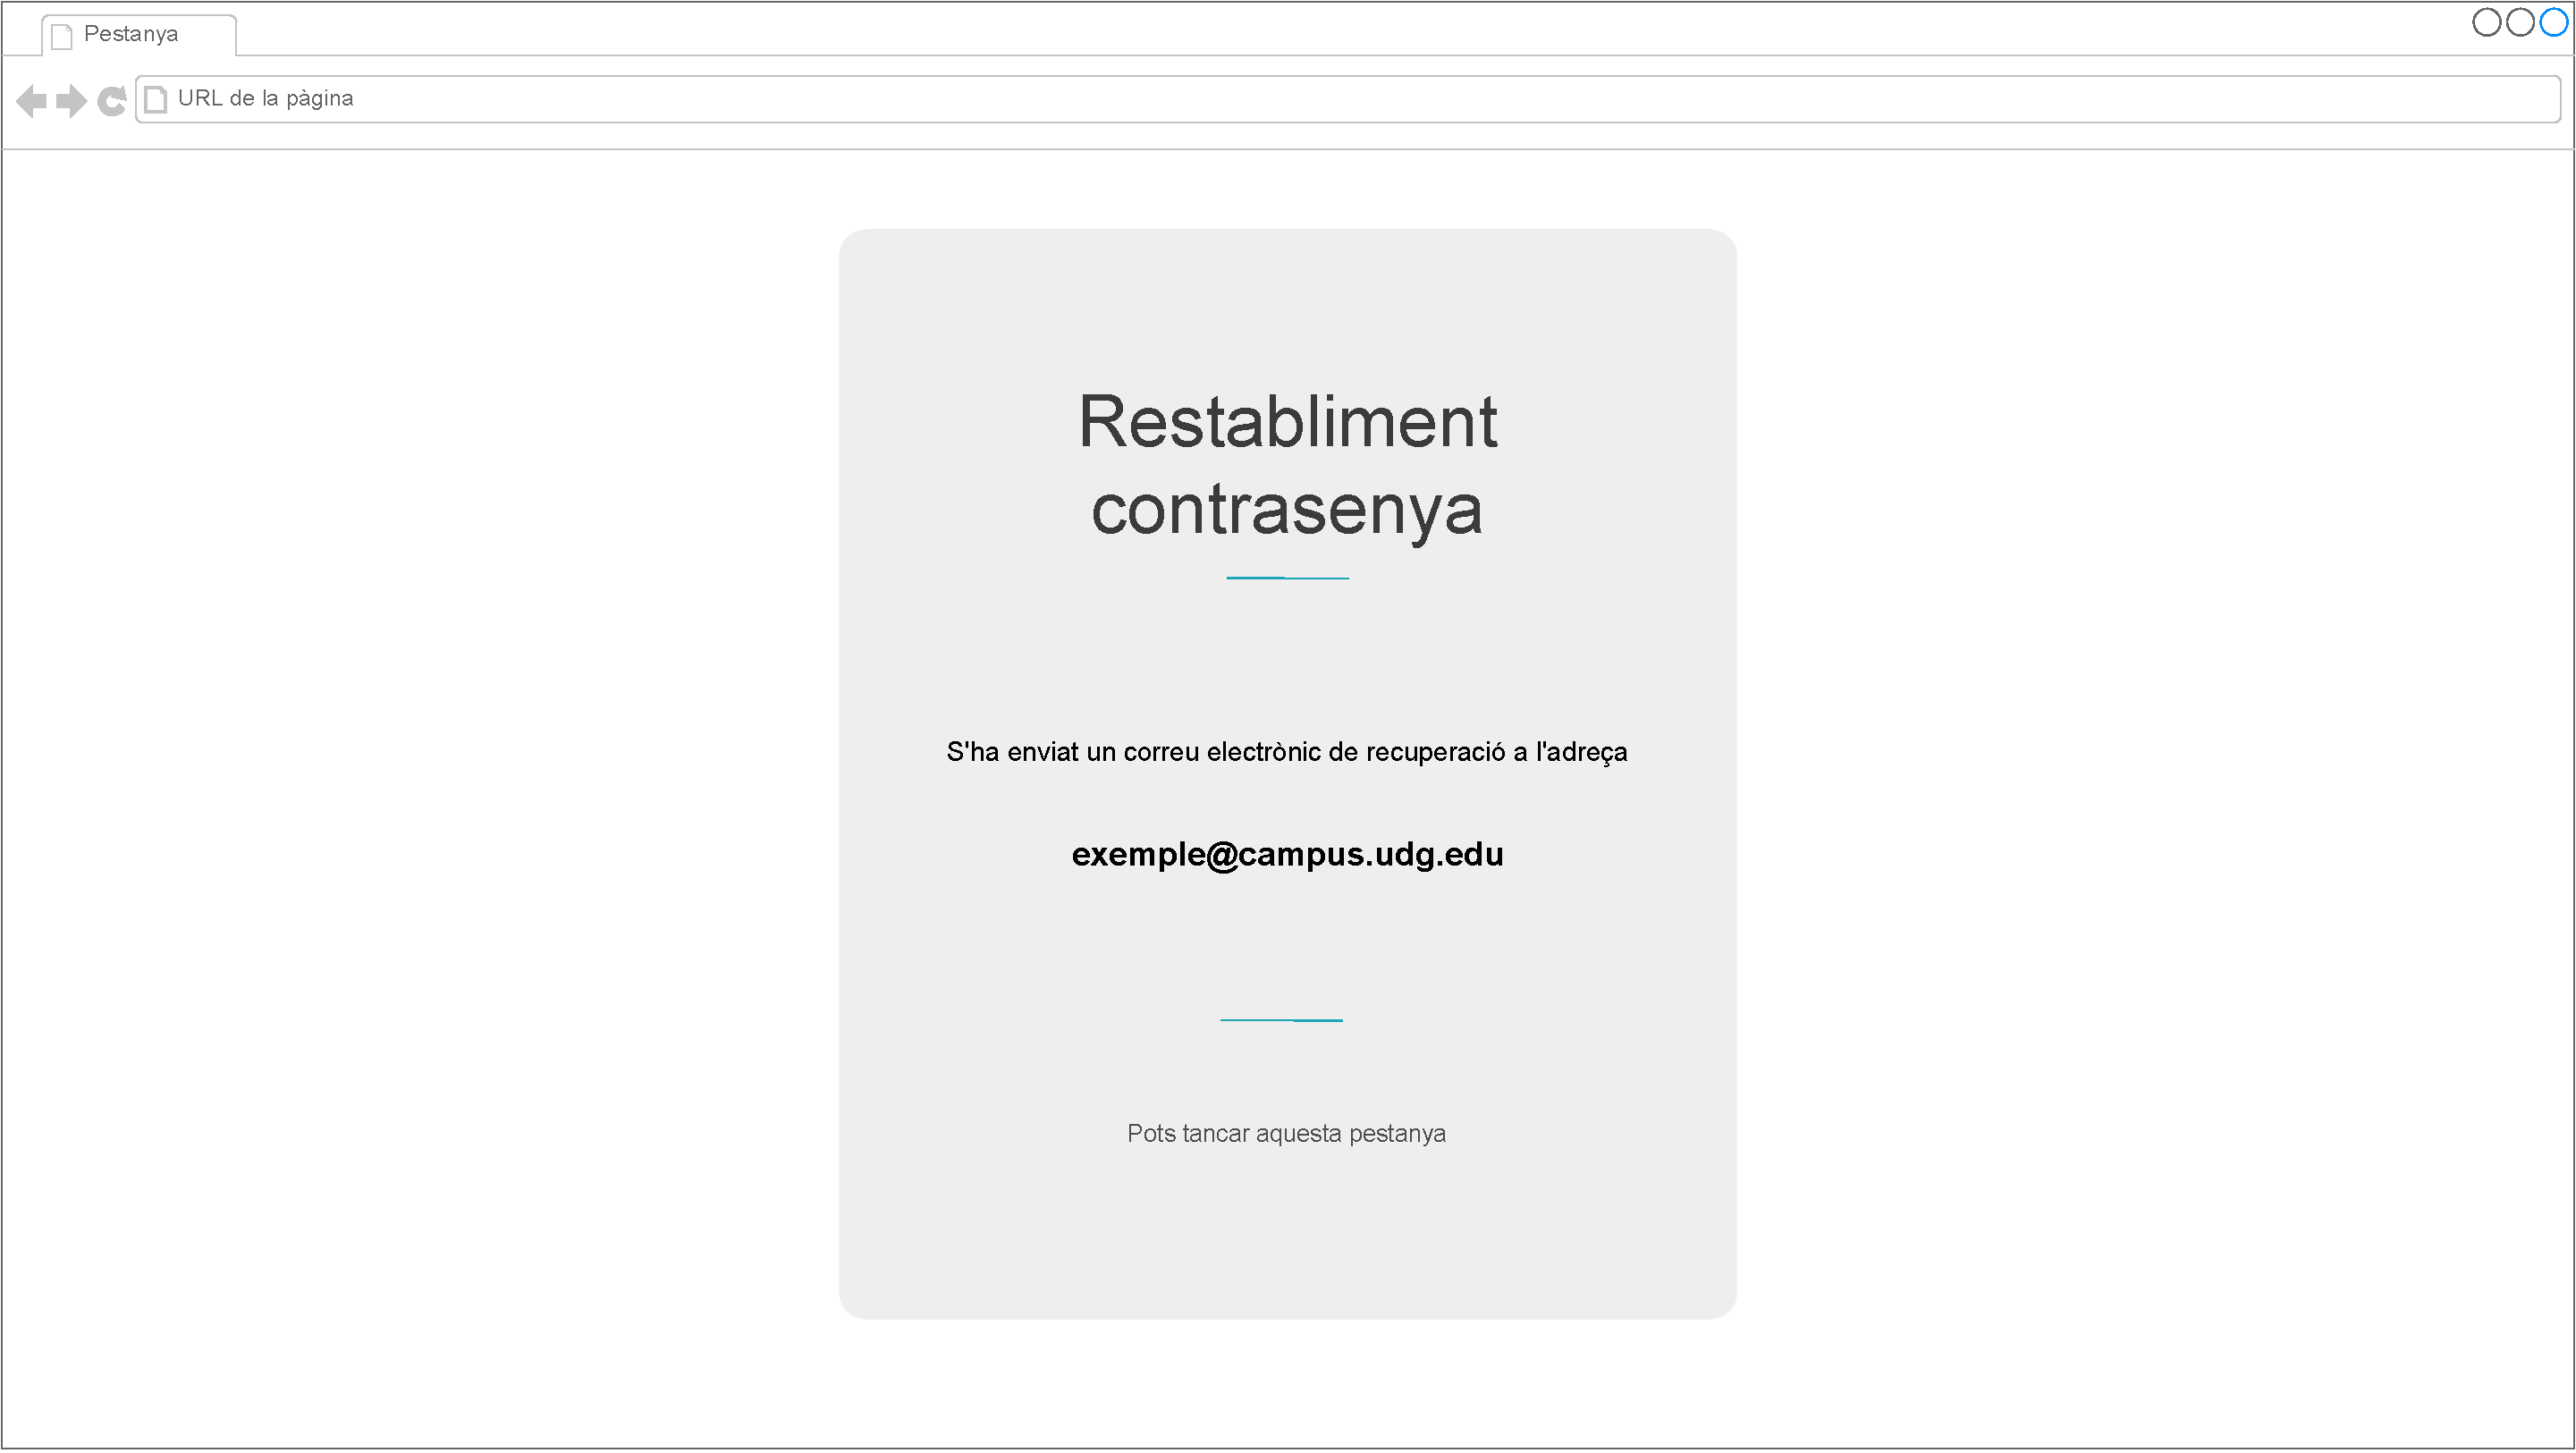
\includegraphics[width=\textwidth]{assets/interfaces/auth/passwordRestablished.pdf}
	\caption{\label{img:passwordRestablished}Disseny de la interfície de confirmació d'enviament d'un \textit{email} per al restabliment de la contrasenya.}
\end{figure}

A la figura~\ref{img:newPassword} es pot veure el disseny de la finestra en la qual l'usuari pot escollir una nova contrasenya.
\begin{figure}[H]
	\centering
	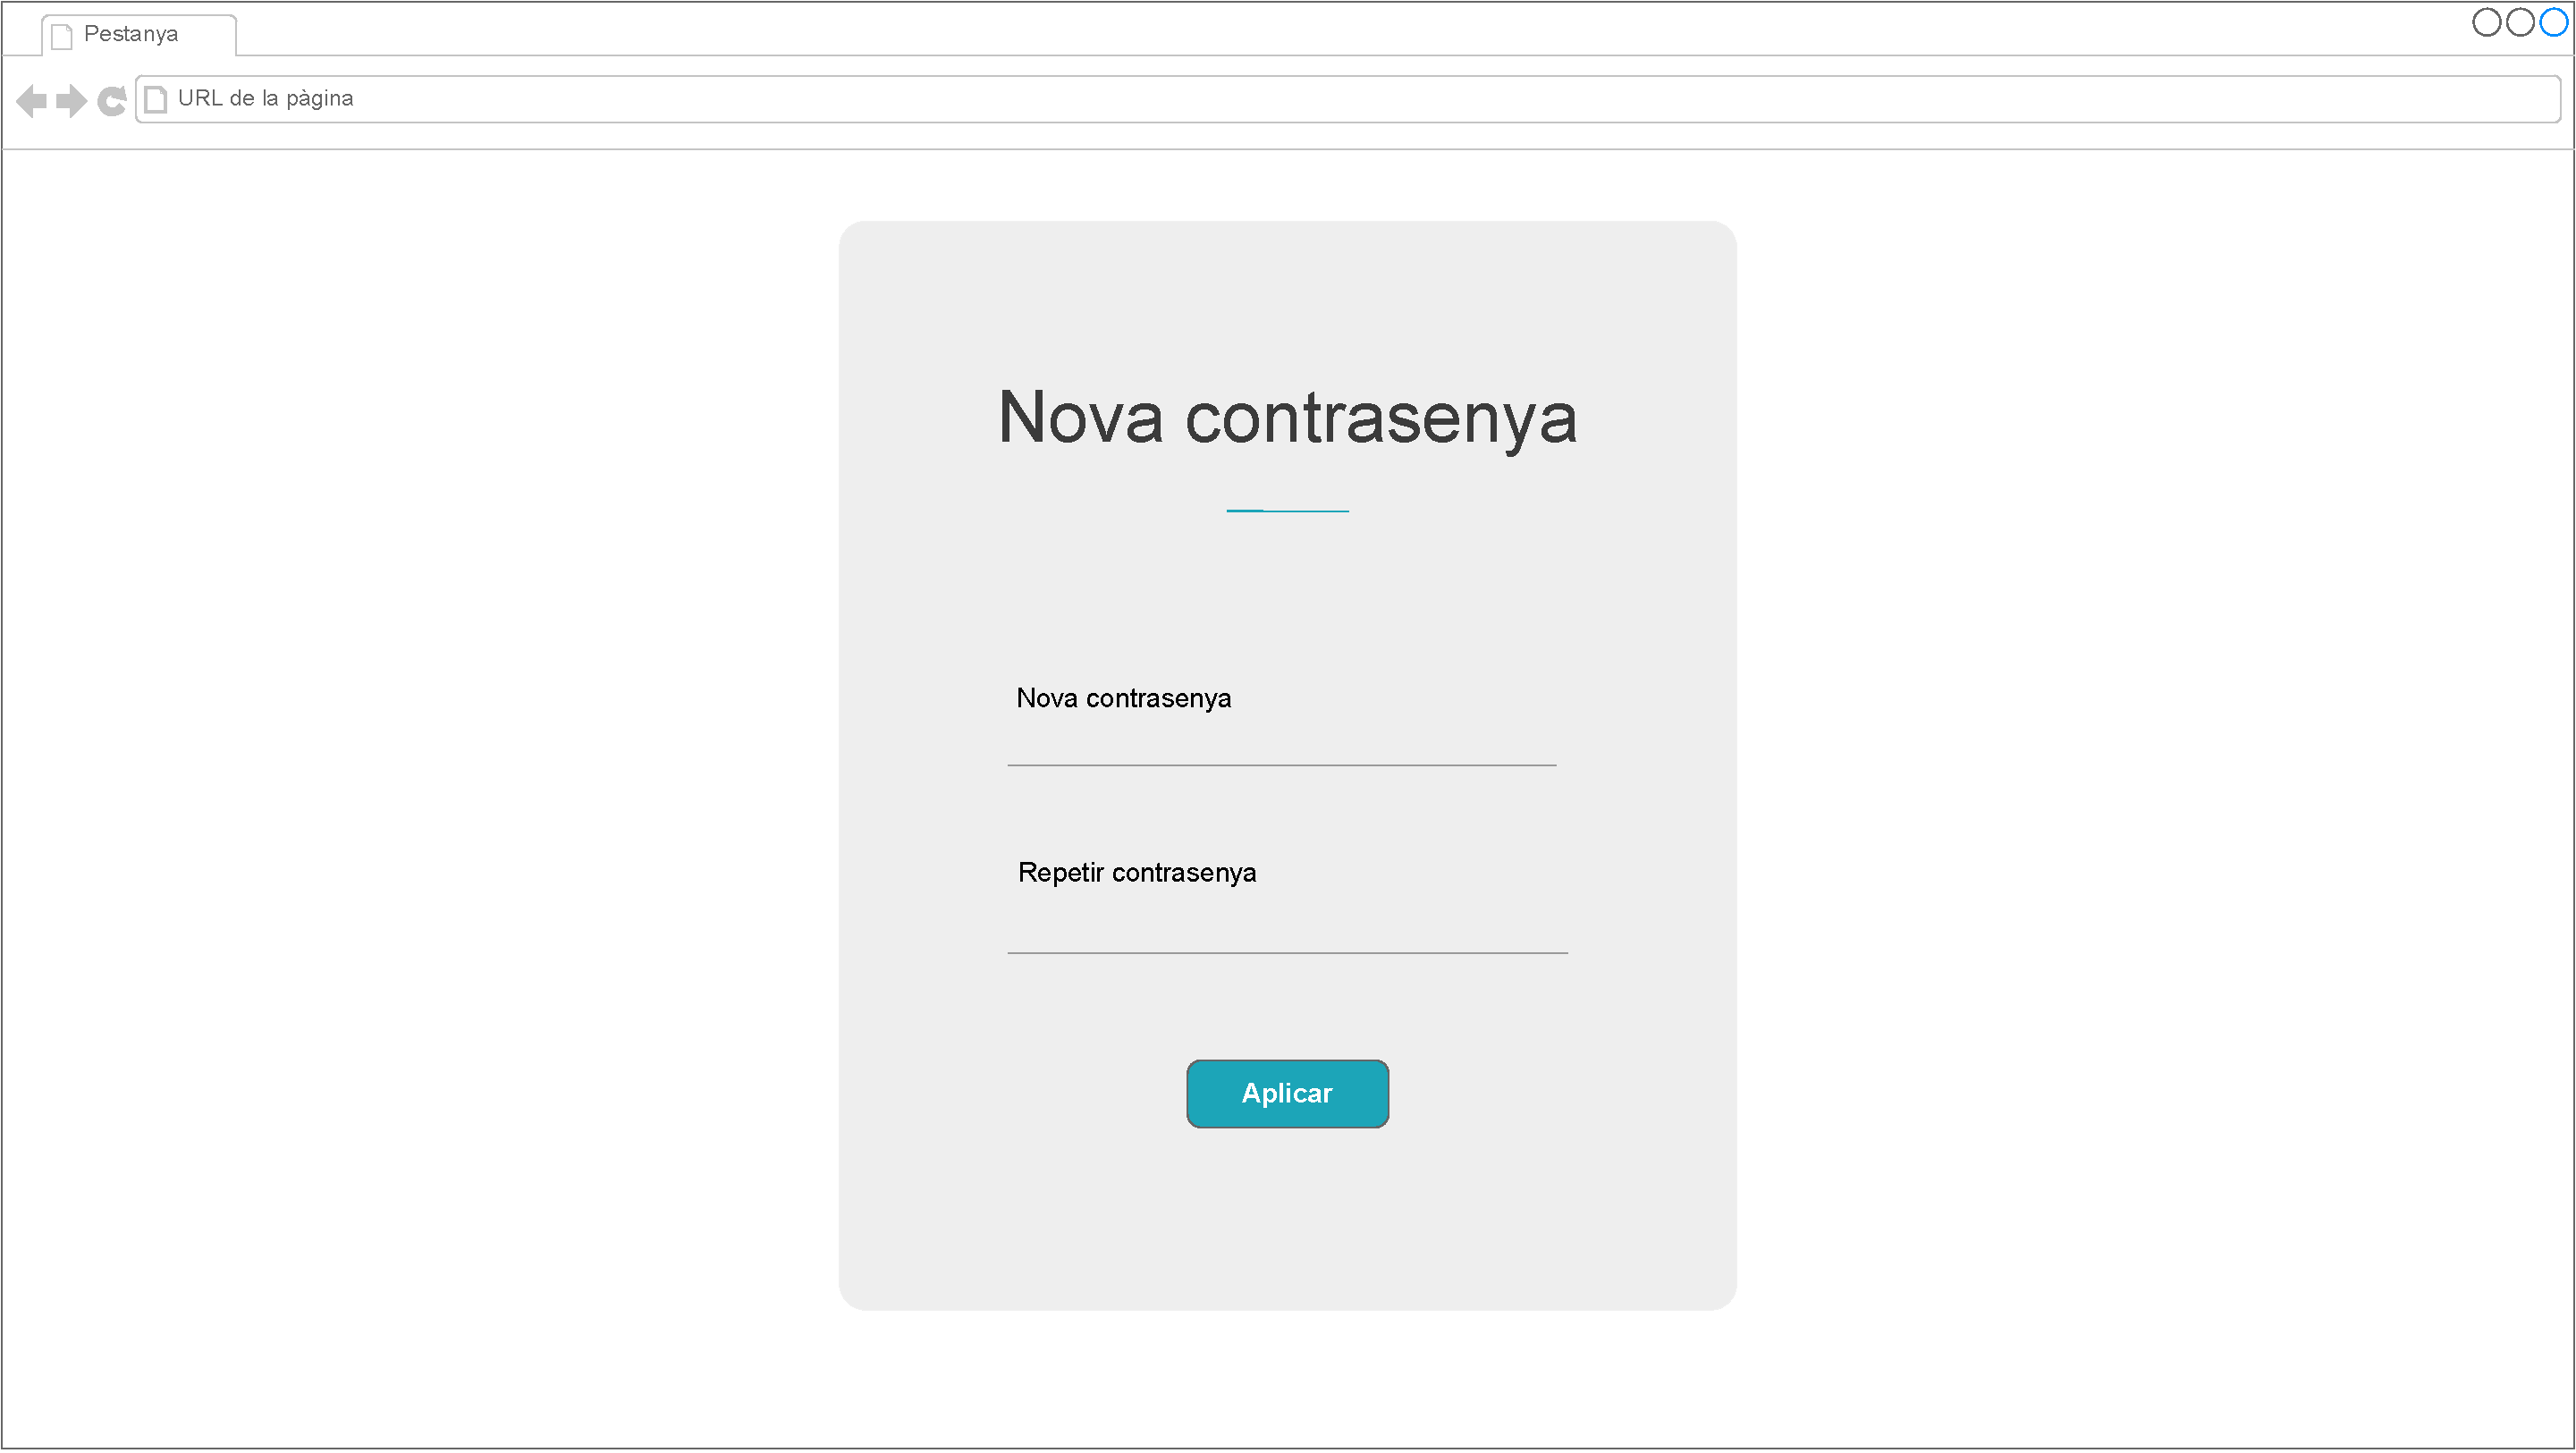
\includegraphics[width=\textwidth]{assets/interfaces/auth/newPassword.pdf}
	\caption{\label{img:newPassword}Disseny de la interfície d'el·lecció d'una nova contrasenya.}
\end{figure}

\subsection{Interfícies de gestió del pla docent}
\label{subsec:interficies_plaDocent}

En aquesta subsecció, es presentarà el disseny de les finestres més importants involucrades en la gestió del pla docent.

A la figura~\ref{img:plaDocent_pujada} es pot veure el disseny de la finestra en la qual un Administrador pot pujar el fitxer d'un pla docent per a la seva facultat i iniciar així el següent curs acadèmic. 

\begin{figure}[H]
	\centering
	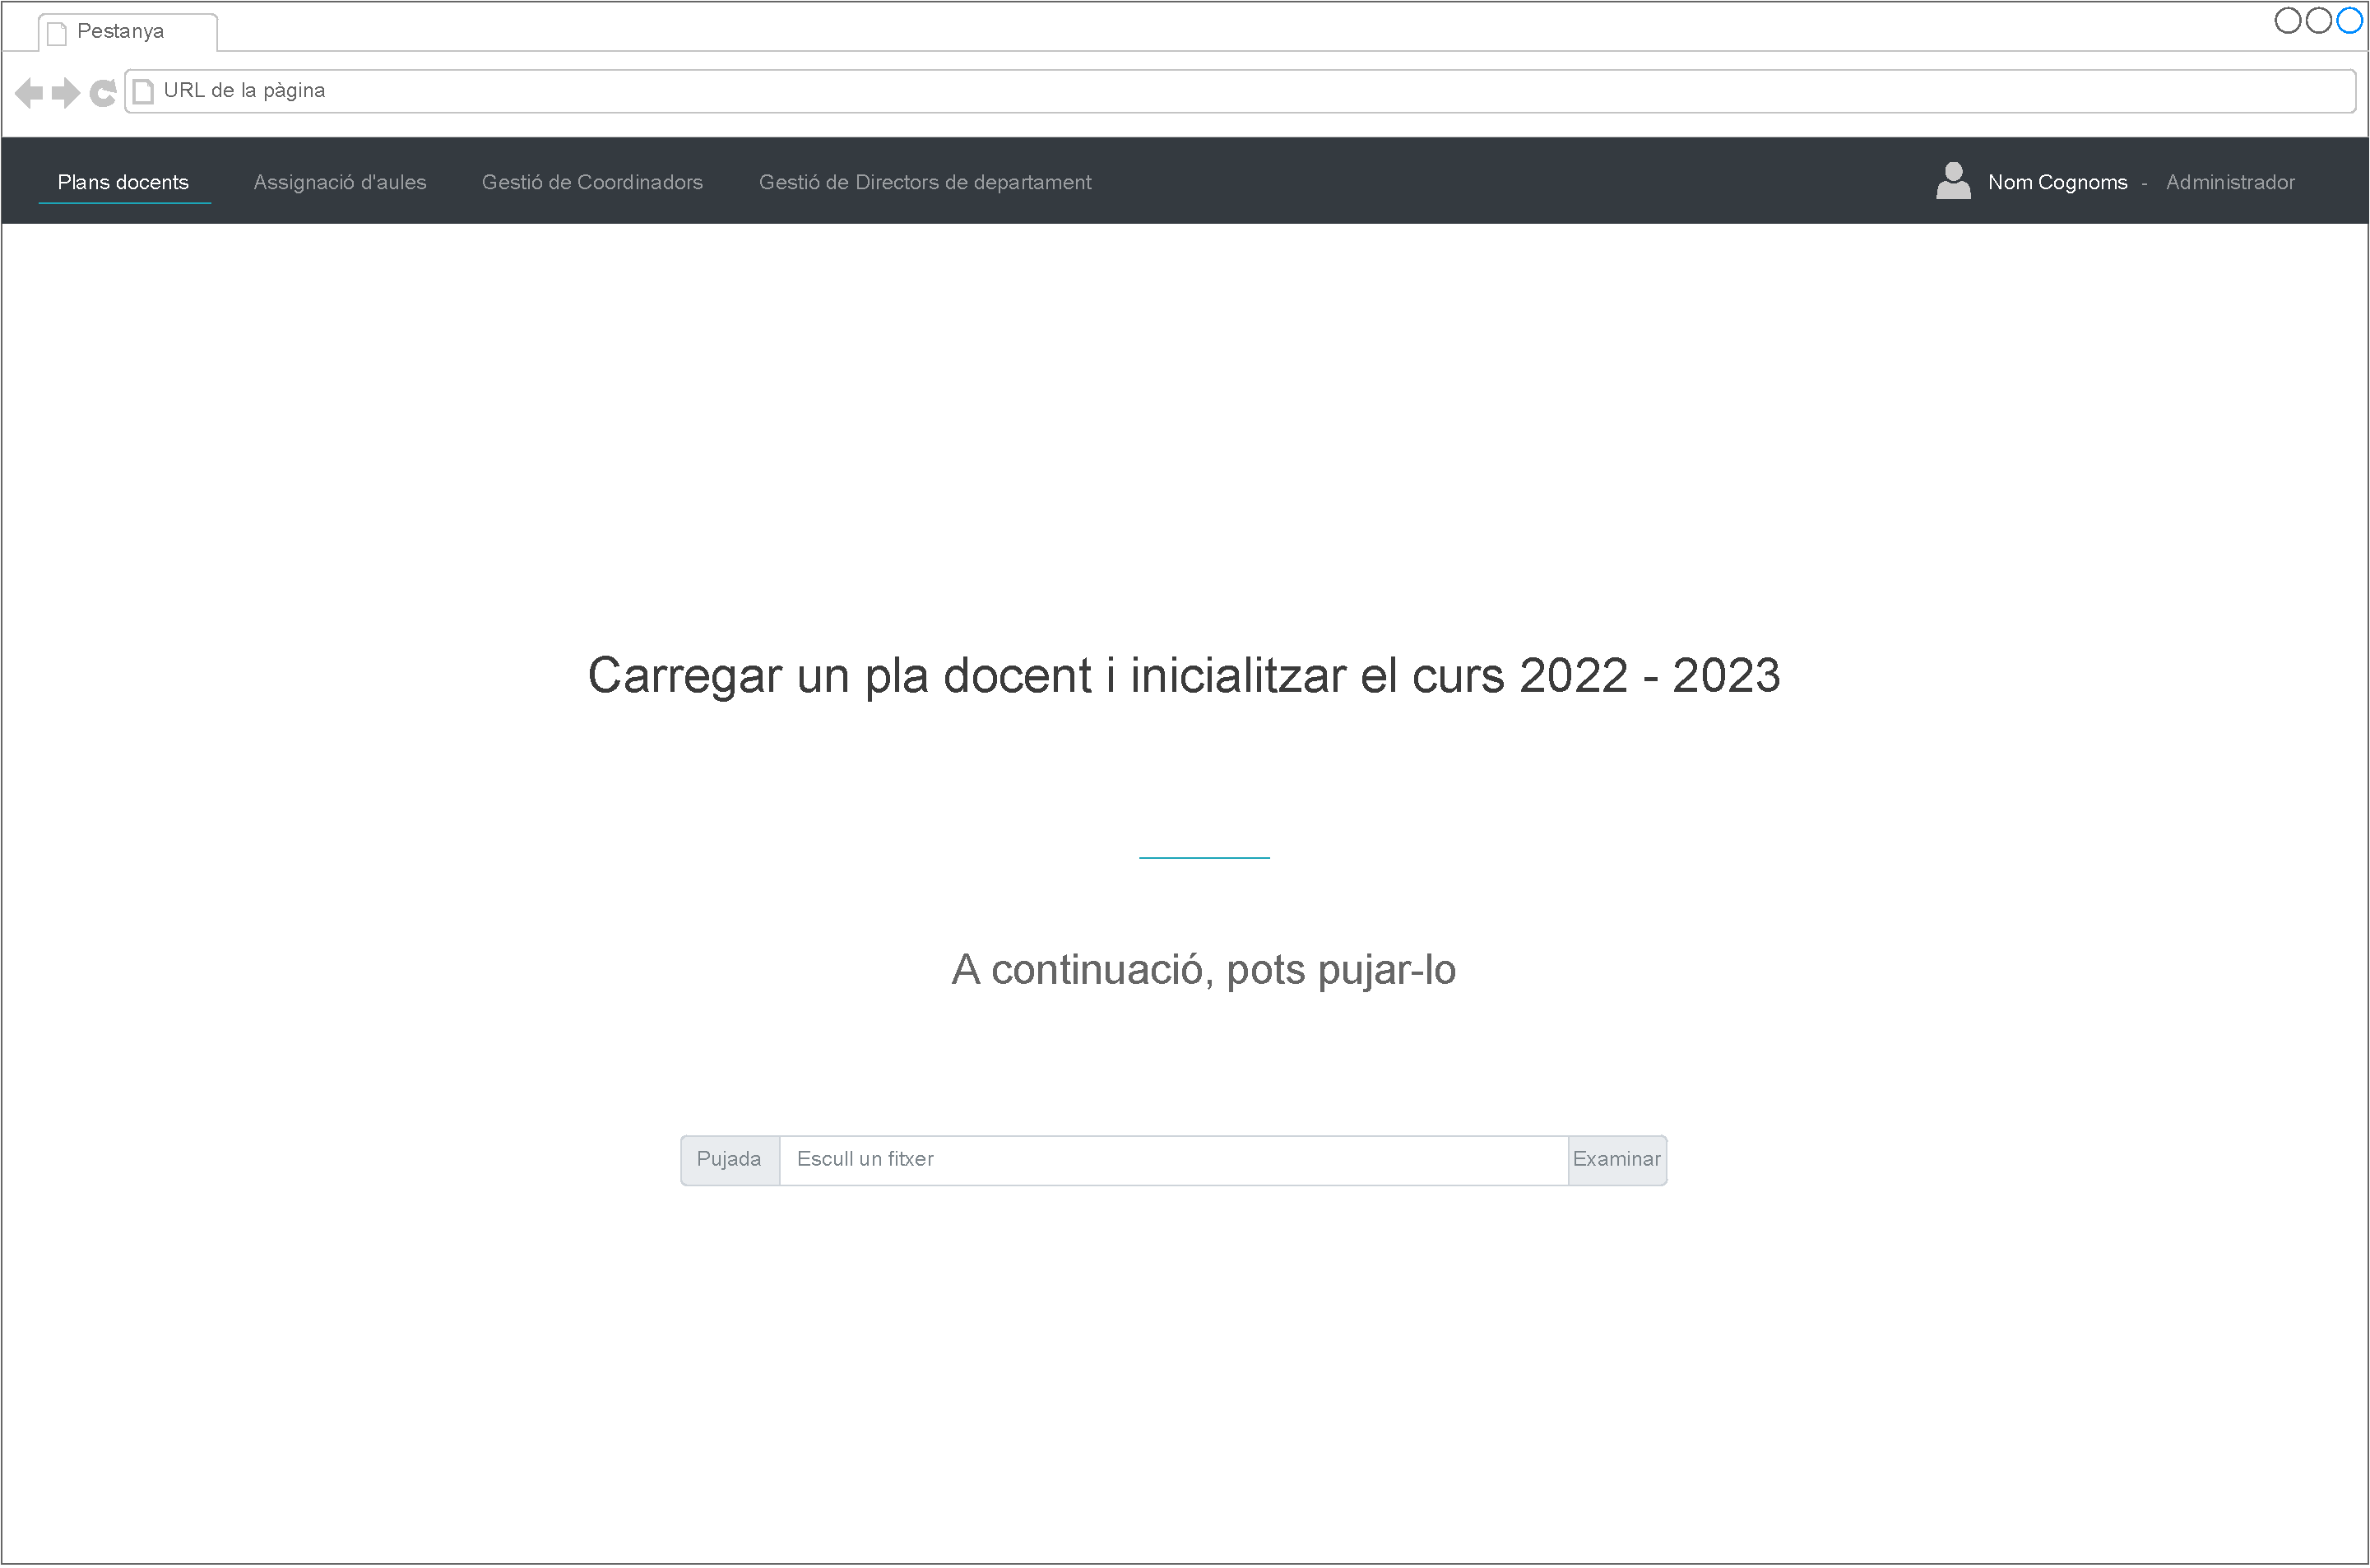
\includegraphics[width=\textwidth]{assets/interfaces/plaDocent/pujada.pdf}
	\caption{\label{img:plaDocent_pujada}Disseny de la interfície de la pujada d'un pla docent.}
\end{figure}

A la figura~\ref{img:plaDocent_general} es pot veure el disseny de la finestra en la qual un Administrador pot consultar la informació general del pla docent actual, accedir a la modificació de les dades pertinents o bé anar a la finestra de pujada d'un pla docent per tal d'iniciar el curs següent.

\begin{figure}[H]
	\centering
	\includegraphics[width=\textwidth]{assets/interfaces/plaDocent/general.pdf}
	\caption{\label{img:plaDocent_general}Disseny de la interfície de gestió del pla docent.}
\end{figure}

\subsection{Interfícies de gestió d'usuaris}
\label{subsec:interficies_gestio_usuaris}

En aquesta subsecció, es presentarà el disseny de les finestres més importants involucrades en la gestió d'usuaris.

Aquests dissenys corresponen a la gestió de Coordinadors i la seva assignació a estudis. No obstant això, també són vàlids per a la gestió de Directors i la seva assignació a departaments, per a la gestió de Responsables de docència i la seva assignació a àrees i per a la gestió de Professors.

A la figura~\ref{img:usuaris_assignacio} es pot veure el disseny de la finestra en la qual un usuari Administrador pot gestionar l'assignació d'usuaris Coordinadors a estudis o bé accedir al seu control.

\begin{figure}[H]
	\centering
	\includegraphics[width=\textwidth]{assets/interfaces/usuaris/assignacio.pdf}
	\caption{\label{img:usuaris_assignacio}Disseny de la interfície d'assignació de Coordinadors a estudis.}
\end{figure}

A la figura~\ref{img:usuaris_assignacio} es pot veure el disseny de la finestra en la qual un usuari Administrador pot controlar usuaris Coordinadors. Més concretament, pot crear-ne, eliminar-ne o bé reenviar el correu electrònic d'activació als que no estiguin activats.
\begin{figure}[H]
	\centering
	\includegraphics[width=\textwidth]{assets/interfaces/usuaris/control.pdf}
	\caption{\label{img:usuaris_control}Disseny de la interfície de control de Coordinadors.}
\end{figure}

A la figura~\ref{img:usuaris_crear} es pot veure el disseny de la finestra en la qual un usuari Administrador pot introduir les dades necessàries per crear nous usuaris Coordinadors.
\begin{figure}[H]
	\centering
	\includegraphics[width=0.4\textwidth]{assets/interfaces/usuaris/crear.pdf}
	\caption{\label{img:usuaris_crear}Disseny de la interfície de creació de Coordinadors.}
\end{figure}

\subsection{Interfícies de consulta i elaboració d'horaris}
\label{subsec:interficies_horaris}

En aquesta subsecció, es presentarà el disseny de les finestres més importants involucrades en la consulta i l'elaboració d'horaris.

A la figura~\ref{img:horaris_seleccioEstudi} es pot veure el disseny de la finestra en la qual un usuari Coordinador pot accedir a les finestres de visualització o de modificació del grau que gestiona o bé a la selecció d'un horari dels estudis els quals comparteixen alguna assignatura amb el seu per tal de visualitzar-lo.

Aquest disseny també és vàlid per a l'accés a la visualització dels horaris dels estudis corresponents per part d'un Director de departament o d'un Professor.

\begin{figure}[H]
	\centering
	\includegraphics[width=\textwidth]{assets/interfaces/horaris/seleccioEstudi.pdf}
	\caption{\label{img:horaris_seleccioEstudi}Disseny de la interfície d'accés a la gestió d'un horari d'un estudi.}
\end{figure}

A la figura~\ref{img:horaris_seleccioProfessor} es pot veure el disseny de la finestra en la qual un usuari Coordinador pot accedir a la visualització d'un horari d'un dels Professors que imparteixen docència al seu grau.

Aquest disseny també és vàlid per a l'accés a la visualització dels horaris dels professors corresponents per part d'un Director de departament o d'un Responsable de docència.

\begin{figure}[H]
	\centering
	\includegraphics[width=\textwidth]{assets/interfaces/horaris/seleccioProfessor.pdf}
	\caption{\label{img:horaris_seleccioProfessor}Disseny de la interfície d'accés a la visualització d'un horari d'un Professor.}
\end{figure}

A la figura~\ref{img:horaris_seleccioAula} es pot veure el disseny de la finestra en la qual un usuari Coordinador pot accedir a la visualització d'un horari d'una aula.

\begin{figure}[H]
	\centering
	\includegraphics[width=\textwidth]{assets/interfaces/horaris/seleccioAula.pdf}
	\caption{\label{img:horaris_seleccioAula}Disseny de la interfície d'accés a la visualització d'un horari d'una aula.}
\end{figure}

A la figura~\ref{img:horaris_visualitzacio} es pot veure el disseny de la finestra en la qual un usuari Coordinador visualitza un horari d'un estudi. A més a més, pot alternar entre les diferents vistes setmanals, accedir al detall d'un bloc horari i tornar a la finestra de selecció d'horaris.

Aquest disseny també és vàlid per a la visualització d'horaris tant de Professors com d'aules.

\begin{figure}[H]
	\centering
	\includegraphics[width=\textwidth]{assets/interfaces/horaris/visualitzacio.pdf}
	\caption{\label{img:horaris_visualitzacio}Disseny de la interfície de visualització d'un horari d'un estudi.}
\end{figure}

A la figura~\ref{img:horaris_modif} es pot veure el disseny de la finestra en la qual un usuari Coordinador visualitza un horari d'un estudi i pot realitzar-hi modificacions: pot crear blocs horaris, arrossegar-ne, canviar-ne la mida, la setmana, etc. A més a més, pot accedir al detall d'un bloc horari i modificar-lo des d'allà. Per últim, pot accedir a un menú d'opcions per modificar certes configuracions, com ara habilitar o deshabilitar opcions de filtratge, de visualització de solapaments, etc.

\begin{figure}[H]
  \centering
  \includegraphics[width=\textwidth]{assets/interfaces/horaris/modif.pdf}
  \caption{\label{img:horaris_modif}Disseny de la interfície de modificació d'un horari d'un estudi.}
\end{figure}


\chapter{Implementació i proves}
\label{cap:implementacio}





\chapter{Implantació i resultats}
\label{cap:implantacio}





\chapter{Conclusions}
\label{cap:conclusions}





\chapter{Treball futur}
\label{cap:treball_futur}

\begin{itemize}
  \item Poder buscar usuaris per consultar les seves dades (nom, rol, departament, telèfon, email, etc.) i habilitar un link per enviar-li un email.
  \item Que l'inicialització dels cursos no es basi en un excel, sinó que es puguin recuperar les dades de les BDD de l'escola.
  \item Sistema d'avisos i notificacions.
  \item Assignar un grup de professors a assignatures en concret, per facilitar l'assignació per part dels responsables de docència.
  \item Que els professors puguin indicar preferències en quant a blocs horaris / grups.
  \item \ldots
\end{itemize}


\backmatter

\bibliographystyle{ThesisStyleBreakable}
\bibliography{biblio}
%\printnomenclature

%\appendix

%\include{Appendix1}

\chapter*{Manual d'usuari}

\section*{Rol 1}



\section*{Rol 2}



\section*{Rol 3}



\section*{Rol 4}




\end{document}
